% 中文論文版本（臺灣碩博士論文章節格式）；與英文稿 paper/en/main.tex 內容一致，數字以 raw_materials/experimental_log.md 為準。
\documentclass[12pt,a4paper,UTF8,fontset=none,openany]{ctexrep}
\usepackage[margin=2.5cm]{geometry}
\usepackage{amsmath,amssymb}
\usepackage{booktabs}
\usepackage{graphicx}
\usepackage{caption}
\usepackage{xcolor}
\usepackage[round,authoryear]{natbib}
\usepackage[hidelinks]{hyperref}
\usepackage{setspace}
\IfFontExistsTF{Noto Serif CJK TC}{%
  \setCJKmainfont{Noto Serif CJK TC}
  \setCJKsansfont{Noto Sans CJK TC}
  \setCJKmonofont{Noto Sans Mono CJK TC}
}{%
  \setCJKmainfont{Noto Sans CJK TC}
  \setCJKsansfont{Noto Sans CJK TC}
  \setCJKmonofont{Noto Sans Mono CJK TC}
}
\ctexset{
  chapter = {name = {第,章}, number = \chinese{chapter}},
  bibname = {參考文獻},
  contentsname = {目錄},
  listfigurename = {圖目錄},
  listtablename = {表目錄},
  figurename = {圖},
  tablename = {表},
  appendixname = {附錄},
}
\setstretch{1.5}
\setlength{\emergencystretch}{3em}
\graphicspath{{../figures/}}

\title{共現不等於流動：AI 與決策之間結構洞前提的預先登錄檢驗}
\author{［作者姓名］\\［系所、學校］}
\date{論文草稿，2026 年 11 月}

\begin{document}
\maketitle
\pagenumbering{roman}

\chapter*{摘要}
\addcontentsline{toc}{chapter}{摘要}
共詞分析與文獻式知識發現係從共現（co-occurrence）解讀結構，而 AI 功能與決策功能之間稀疏的共現，很容易被解讀為人工智慧（AI）與管理決策之間存在結構洞（structural hole）。本研究所屬的專案曾作出此一推論，並據以建構多層規劃（MLP）模型。本研究說明為何共現無法承載此一構念，並以流動資料檢驗此一前提。研究一：16 個偏低的功能配對在不同隨機種子與時期之間維持其方向（在排除同詞兩端共用紀錄的規則式關鍵詞矩陣中為 13 個），但在實際可能的誤分類水準下即失去顯著性；此方向僅屬描述性。研究二對 8,512,829 件美國發明專利進行八項預先登錄的分析（其中僅一項為驗證性分析），另加一項探索性描述。AI 專利與決策專利相互引用的程度遠高於依時間分層的期望值（OE 3.05，95\% CI 2.94--3.17）；兩項相對的結構洞判準在全部六項敏感度分析中皆未成立，在移除所有帶有 G06Q10/04 分類碼的專利後亦未成立（OE 3.16）。在 16,703 組專利技術領域配對中，共現缺口同時為流動缺口的比例為 66.8\%（隨機基準為 25\%），另有 7.0\% 的流動高於期望值；以分類距離解釋兩者不一致的預先登錄假說則未獲支持。專門型 AI 公司與專門型決策公司之間的分隔，超出保留專利組合之虛無模型所能解釋的範圍（$p = .001$）：該虛無模型重現了與均等（parity）之差距的 85--91\%，但專門型公司之間的連結仍比其期望值低 22--33\%。由於沒有任何有效的虛無模型能同時固定公司度數，此一分隔尚未在固定度數下受檢驗，公司層次的中介亦仍未解決。一項預先登錄、以模型編碼的系統性文獻回顧涵蓋 204 篇已索引（indexed）研究，在其摘要中發現：135 篇提出結構洞或中介者主張，其中 73 篇建立在專利網路上；而 66 項缺口主張中有 46 項未報告任何基準。未能發現知識流動中的結構洞，並不足以確立組織層面瓶頸的存在；一項規劃中的企業研究將檢驗各項競爭解釋。


\noindent\textbf{關鍵詞：}結構洞；人工智慧；決策；專利引用；預先登錄；多層規劃

\tableofcontents
\listoffigures
\listoftables

\clearpage
\pagenumbering{arabic}
% 第一章 緒論（對應英文稿 Section 1, en/front.tex）
\chapter{緒論}
\label{zh:sec:intro}

管理與資訊系統研究日益將人工智慧（artificial intelligence, AI）視為組織決策的問題。此類研究探討結合人類與 AI 決策者的決策結構 \citep{shrestha2019organizational}、管理任務之自動化與增強兩者間的相互依存 \citep{raisch2021artificial}、人類與 AI 在組織決策中的互補角色 \citep{jarrahi2018artificial}，以及 AI 的自主性、學習能力與難以解讀性所帶來的獨特管理挑戰 \citep{berente2021managing}。這些文獻皆未主張 AI 與決策之間存在結構洞（structural hole），本研究亦不將此一主張歸於它們。

此一主張其實源自某一特定類型的證據。從共現（co-occurrence）解讀結構是一種既有的做法。共詞分析（co-word analysis）依據關鍵詞的共現，描繪研究主題之間的關係或關係之闕如 \citep{callon1983translations}；文獻式知識發現（literature-based discovery）則將從未被共同引用或共同提及的文獻視為彼此無連結，並以此一闕如產生關於兩者間連結的假說 \citep{swanson1986fish}。依此類推，當 AI 功能與決策功能鮮少被同時提及時，人們很容易推論其背後的社群彼此分隔。以網路的語彙而言，此一推論指向結構洞：非冗餘聯繫對象之間的分隔，使跨越此分隔的行動者獲得資訊與控制上的利益 \citep{burt1992structural}，對管理者而言則帶來更好的構想 \citep{burt2004structural}；弱連帶則是跨越此類分隔的經典管道 \citep{granovetter1973strength}。本文所報告的研究專案將同一推論套用於 AI 與決策，而本研究即檢驗流動資料是否支持此一推論。該專案凍結的 V9 分析以文獻共現矩陣為對象，發現 16 個偏低（depleted）的 AI 功能族與決策功能族配對。專案將其解讀為 AI 與決策之間的結構性分隔，並據以建構一個多層規劃（multi-level programming, MLP）模型，描述組織如何分配資源、治理 AI，以及配置人機決策。因此，本研究所檢驗的前提，是專案本身由共現證據導出的工作前提，而非取自所引文獻的立場。

從共現推論至結構洞並不成立，而說明其原因是本研究的第一個目的。結構洞係定義於以真實資訊或資源交換關係相連之行動者的自我中心網路（ego network）上，且結構洞的測量指標各自適用於特定的資料類型（第~\ref{zh:sec:theory_holes}~節）。共現記錄的是隸屬關係，而非流動（flow）：在嚴格的二模網路（two-mode network）中，網路限制度（Burt constraint）的間接項會消失，而單模投影（one-mode projection）則會製造出封閉性（第~\ref{zh:sec:theory_cooccurrence}~節）。有效的檢驗需要帶有群組標籤之行動者之間的有向二元（dyadic）流動。專利引用長久以來被用作知識流動的證據 \citep{jaffe1993geographic}，能在母體規模上提供此類資料，且其標籤由審查員指派。本研究的第二個目的，即是在預先登錄（preregistration）之下，以此類資料檢驗該前提。

本研究探討三組研究問題。\textbf{RQ1：}AI 與決策作為知識領域，兩者之間是否存在結構洞？\textbf{RQ2：}若在領域層次並不存在，則在組織（公司）層次，於公司技術組合在機制上所隱含者之外，是否存在結構洞？\textbf{RQ3／RQ4：}根據上述答案，對於專案模型關於整合問題所在位置的設定，可得出何種推論？又應如何區辨各項競爭解釋（competing explanations）？

證據來自三條資料線（圖~\ref{zh:fig:research_design}）：文獻（研究一）、六個公開關係資料來源的篩檢，以及美國發明專利（utility patents）的母體（研究二）；在研究二中，AI 為 CPC G06N，決策（decision-making, DEC）為 CPC G06Q10/04 加上 G06Q10/06。研究二包含五項預先登錄的分析（計畫 1至計畫 5）。這些計畫是專案自有儲存庫中自行加註時間戳記的提交（commit），且計畫 2至計畫 5皆是在先前結果已知之後才撰寫的（第~\ref{zh:sec:design_prereg}~節）。研究三為一項規劃中的企業研究，不報告任何結果。

在知識流動層次，研究發現為否定性的。AI 專利與決策專利相互引用的比率約為期望值的三倍（觀察值對期望值強度〔observed-to-expected intensity, OE〕為 3.05）；兩項預先登錄的結構洞相對判準皆未成立，且判定 \texttt{HOLE\_\allowbreak NOT\_\allowbreak SUPPORTED} 在全部六種敏感度分析（sensitivity analysis）設定以及三項構念效度（construct validity）檢查（排除 G06Q10/04；匹配參照集粒度）中皆維持不變，惟部分過度連結（over-connection）可能是近乎機械性的（第~\ref{zh:sec:study2_aggregate}~節；表~\ref{zh:tab:construct}）。在公司層次，專門型（specialist）AI 公司與決策公司之間的連結少於期望，且超出專利組合構成所能解釋的分隔具有顯著性（兩種分層方式下皆為 $p = .001$）。其大小取決於所採用的尺度：在「與 1 之差距」尺度上，保留專利組合的虛無模型（portfolio-preserving null）重現了其中的 85\% 與 91\%；而在比值尺度上，專門型公司之間的連結分別為虛無模型期望值的 0.67 與 0.78，即短少 33\% 與 22\%。混合型（多角化）公司是否扮演此一分隔的中介者（broker），仍未解決。度數匹配的虛無模型顯示這類公司的限制度較低，但專利組合虛無模型並未固定度數，且沒有任何現有的虛無模型能同時固定兩者。因此，預先登錄的判定 \texttt{PARTIAL} 意指公司層次的結構洞未獲證實，但亦未被排除（第~\ref{zh:sec:study2_firm}~節）。在文獻中，16 個偏低功能配對的方向在不同隨機種子、編碼軌（tracks）與時期之間皆穩定，且在移除同詞兩端共用（same-term self-pairing）的紀錄後大致仍然成立；然而，其顯著性在實際可能的誤分類（misclassification）水準下無法維持，而模型推論的標籤仍是一項未經檢驗的非隨機誤差來源（第~\ref{zh:sec:study1}~節）。

這些結果移除了專案模型的一項正當性依據，卻未提供另一項。關於 AI 為何未能充分整合進管理決策，有數種解釋相互競爭——組織的資源分配（resource allocation）與決策權（decision rights）、資料品質、成本、法規與責任歸屬，以及任務適配性——而研究一與研究二並未偏向其中任何一項（第~\ref{zh:sec:discussion_hypothesis}~節）。MLP 模型僅將組織層面的候選解釋形式化，而研究三旨在區辨這些候選解釋，而非證實其中之一。

本研究有四項貢獻。第一，本研究說明為何從共現推論至結構洞是無效的，並在專案本身的資料中記錄四種失效模式：投影所生的團（projection cliques）、限制度在二分網路（bipartite network）上的退化（一項恆等式）、同詞兩端共用，以及模型推論的標籤。前兩者在社會網路分析中已為人所知：投影會產生封閉性 \citep{opsahl2013triadic}，投影後的中介並非二模中介 \citep{jasny2015two}，而限制度受度數與二元連帶所驅動 \citep{everett2020unpacking}。本研究並不主張發現了這些問題；本研究的貢獻在於完整追溯其對缺口推論的後果，從文獻矩陣一路延伸至以流動資料進行的檢驗。第二，本研究在五項預先登錄計畫下以有向流動資料檢驗該前提，並說明此一預先登錄能證明與不能證明之處。第三，本研究報告一項明確的否定結果。第四，本研究提出兩個陳明其限制的虛無模型（null model）：一是針對區塊結構文件的 M06-P（專利適用之保留文件結構虛無模型）——標準的交換虛無模型在此類文件上會退化——此模型並無獨立的型一誤差校準；二是保留專利組合的公司虛無模型，其並未保留公司的度數。對 MLP 研究議程的意涵係由上述結果推導而來，並非另一項研究發現。

第~\ref{zh:sec:theory}~章與第~\ref{zh:sec:design}~章闡述理論與研究設計，第~\ref{zh:sec:study1}~節與第~\ref{zh:sec:study2}~節報告研究一與研究二，第~\ref{zh:ch:discussion}~章整合各項證據，第~\ref{zh:sec:mlp}~節推導對 MLP 研究議程的意涵，第~\ref{zh:sec:limitations}~節與第~\ref{zh:sec:conclusion}~章討論研究限制並作出結論。附錄~\ref{zh:app:prereg}～\ref{zh:app:mlp} 收錄預先登錄紀錄、敏感度分析表與模型細節。

% 第二章 文獻探討（對應英文稿 Section 2, en/front.tex）
\chapter{文獻探討}
\label{zh:sec:theory}

\section{結構洞及其測量}
\label{zh:sec:theory_holes}

結構洞（structural hole）是自我中心網路（ego network）中非冗餘聯繫對象之間的分隔。若一行動者的聯繫對象彼此並不相連，該行動者便能獲得非冗餘的資訊，並能使聯繫對象相互牽制；此即中介（brokerage）的資訊利益與控制利益 \citep{burt1992structural}。有論者主張，跨越結構洞的管理者擁有較佳的構想，而此一意義下的中介以真實的連帶與可觀察的結果為前提 \citep{burt2004structural}。此一論點援引了一項較早的觀察：弱連帶能跨越群體傳遞資訊，而強連帶則傾向於在社群內部相互重疊 \citep{granovetter1973strength}。

Burt 用以衡量此類機會之闕如的指標為網路限制度（network constraint；Burt constraint）：
\begin{equation}
c_i \;=\; \sum_{j \in N(i)} \Bigl( p_{ij} + \sum_{q \neq i,j} p_{iq}\, p_{qj} \Bigr)^{2},
\label{zh:eq:constraint}
\end{equation}
其中 $N(i)$ 為 $i$ 的聯繫對象集合，$p_{ij}$ 為 $i$ 對 $j$ 之連帶的比例強度，亦即該連帶權重占 $i$ 全部連帶權重的比例 \citep{burt1992structural}。直接項 $p_{ij}$ 記錄 $i$ 的網路有多少投注於 $j$。間接項 $\sum_{q} p_{iq} p_{qj}$ 記錄此一投注有多少係經由本身亦與 $j$ 相連的第三方 $q$ 而再次觸及 $j$。當 $i$ 的連帶集中於少數聯繫對象，且這些聯繫對象彼此相連時，限制度便高。低限制度被解讀為能接觸到結構洞。

有三條批評路線與此指標的使用方式相關。第一，限制度受度數與二元連帶所驅動；它並非一個衡量排他性中介的單純 0--1 指標 \citep{everett2020unpacking}。因此，除非固定度數，否則比較不同行動者群體的限制度，同時也是在比較其度數。第二，限制度主要操作化的是二元層次的構念（替代選項、夥伴多樣性與集中度），而非更廣泛的網路結構。這要求重新詮釋結構洞的研究發現，但並未否證該理論 \citep{johnson2026reassessing}。第三，不同的結構洞指標適用於不同的資料類型，不能任意相互替代 \citep{saglietto2020research}。中介中心性（betweenness centrality）係指其他節點配對之間的最短路徑中通過某一節點的比例 \citep{freeman1977set}，常被用來篩選中介者，但單憑高中介中心性分數，並不足以確立 Burt 意義下的中介。

一個要求更高的中介定義是關係性且以群體為基礎的。\citet{gould1989structures} 以有向的開放二步路徑 $s \rightarrow v \rightarrow t$（且不存在直接的 $s \rightarrow t$ 連帶），結合 $s$、$v$ 與 $t$ 的群組成員身分，定義了五種中介角色。\citet{zador2022weighted} 將這些角色擴展為加權且標準化的測度，以避免二值化所造成的資訊損失。兩種表述皆要求連帶具有方向，且行動者帶有群組標籤。

本研究從上述文獻中歸納出一項要求，並將其貫徹全文：要檢驗兩個領域之間的結構洞，有效的檢驗需要帶有群組標籤之行動者之間的有向二元流動關係 \citep{gould1989structures}，亦即 Burt 構念所預設的那種真實連帶 \citep{burt2004structural}。在隸屬圖上計算限制度，或在投影網路上計算中介中心性，或許能描述結構，但並不能檢驗 Burt 的構念。因此，研究二將由審查員標記之群組之間的有向申請人引用（applicant citation）與一個相對參照集進行比較，並且僅在保留專利組合的虛無模型（portfolio-preserving null）下，將 Burt 限制度應用於公司對公司的引用網路（第~\ref{zh:sec:study2}~節）。

\section{作為知識領域的 AI 與決策}
\label{zh:sec:theory_domains}

緒論所回顧的管理與資訊系統研究，將 AI 與決策的交會視為組織設計的問題 \citep{shrestha2019organizational,raisch2021artificial,jarrahi2018artificial,berente2021managing}。本研究所檢驗的前提——屬於本研究專案，而非這些作者——對知識提出了較為狹義的主張：AI 與決策構成彼此分離、少有連結的知識體系。本研究據此將兩個領域操作化。在研究一中，領域是從文獻中的證據句編碼而得的功能族：10 個 AI 功能族與 12 個決策功能族，共計 120 格。在研究二中，領域是一組由審查員指派的合作專利分類（Cooperative Patent Classification, CPC）標籤。AI 為 G06N。DEC 為 G06Q10/04（預測與最佳化）加上 G06Q10/06（資源、工作流程、管理與決策分析）。由於預測與最佳化在方法上與機器學習重疊，AI--DEC 之間的任何連結都可能有一部分是近乎機械性的；因此第~\ref{zh:sec:study2_aggregate}~節亦檢驗僅以 G06Q10/06 定義 DEC 的情形。

專利引用記錄一項發明所依據的先前技術，長久以來被用作知識流動（knowledge flow）的證據 \citep{jaffe1993geographic}。然而，有相當大比例的引用是由審查員加入的，這影響其作為流動測度的用途；應區分發明人或申請人引用與審查員引用（examiner citation）\citep{alcacer2006patent}。因此，研究二的主要設定僅使用申請人引用，並以一項預先登錄（preregistered）的敏感度分析（sensitivity analysis）納入所有引用類別。資料取自 PatentsView 的核准專利資料表，其提供專利、現行 CPC 分類、引用及經消歧的受讓人（assignee）資料 \citep{uspto2026patentsview}。

領域檢驗必須是相對的。引用具有領域在地性，因此幾乎任何兩個領域之間的 OE 都低於 1，若採絕對判準，幾乎每一對領域都會被標記為分隔。因此，研究二探問：相較於 179 個可比較的 CPC 大組（CPC main group）（H1a）以及其他商業方法（H1b），AI--DEC 配對是否異常地弱連結；第~\ref{zh:sec:study2_aggregate}~節提供正式定義，以及粒度匹配的 H1a 檢查。

同樣的知識流動也發生在組織之間。公司（firm）持有專門的 AI 專利組合、專門的決策專利組合或混合型組合，而將兩者結合的經濟行動，鑲嵌於組織之間與組織內部的具體關係之中 \citep{granovetter1985economic}。RQ2 探問在此一層次上，是否存在公司專利組合尚未解釋的分隔。

\section{為何共現不等於流動}
\label{zh:sec:theory_cooccurrence}

許多可能被當作 AI 與決策之間「缺口」證據的材料，包括研究一的矩陣，都屬於共現（co-occurrence）：同一篇論文中同時提及某一 AI 功能與某一決策功能，或兩個組織參與同一專案。此類資料屬於二模（two-mode）資料，亦即隸屬（affiliation）資料。它們將行動者連結至事件，而非將行動者彼此相連，且不記錄任何移轉的方向。在此類資料中，稀疏的共現表示兩個標籤很少出現在同一份文件中；它並不表示知識未能在其背後的人或組織之間流動（flow）。

將限制度應用於嚴格的二分網路（bipartite network）會產生一項形式上的後果。設 $i$ 屬於其中一模。則每一個聯繫對象 $j \in N(i)$ 皆屬於另一模，每一個滿足 $p_{iq} > 0$ 的第三方 $q$ 亦然。由於 $q$ 與 $j$ 屬於同一模，兩者不可能相連，故 $p_{qj} = 0$，而式~\eqref{zh:eq:constraint} 中的間接項恆等於零。限制度化約為 $c_i = \sum_{j} p_{ij}^{2}$。若再加上 $i$ 的所有連帶權重皆相等，則對 $i$ 的 $k_i$ 個聯繫對象而言，各 $p_{ij} = 1/k_i$，且 $c_i = 1/k_i$。在此等權條件下，限制度除度數之外不攜帶任何資訊。由於這是一項恆等式，研究一的 Gap Validity 附屬分析（sidecar）與研究二的模組 P9 所報告的零間接項，只是對程式實作的檢查，而非實證證據。兩者在偏低格（depleted cell）周圍所發現的替代路徑亦是如此：在稠密的二分矩陣中，此類路徑幾乎必然存在。

投影無法修補此一問題。例如，共同著作網路是將論文—作者二模資料投影為單模而建構的 \citep{newman2001scientific}，而本研究並不將共同著作視為知識流動的直接證據。單模投影（one-mode projection）會創造人為的封閉性，這正是群聚（clustering）必須針對二模資料重新定義的原因 \citep{opsahl2013triadic}。在投影後計算的中介，並非 \citet{gould1989structures} 意義下開放二步路徑上的中介，因為投影恰恰封閉了這些角色賴以定義的二步路徑；二模中介鏈是一種替代做法 \citep{jasny2015two}。本研究自身的資料說明了此一扭曲的程度。在本研究所篩檢的 CORDIS H2020 專案資料中，經關鍵詞比對之組織的共同成員身分投影包含 1,049 個節點與 12,181 條邊。它產生了 102,660 個專案內三元組（triad），然而僅有 156 條邊在 $\geq 2$ 個專案中重複出現。

研究一另揭示了兩種失效模式：同詞兩端共用（same-term self-pairing），即同一個詞被編碼於配對的兩端；以及人工信度偏低的模型推論標籤（第~\ref{zh:sec:study1_direction}~節與第~\ref{zh:sec:study1_reliability}~節）。兩者皆非隨機雜訊。在邊際固定的封閉矩陣中，因編碼錯誤而膨脹的一格，會提高同列與同欄其他格的期望次數，因此系統性錯誤可能製造出偏低，而不僅是使其模糊。

Burt 的構念需要帶有標籤之行動者之間的有向二元流動。原則上，引用可以提供此類流動：施引文件汲取被引文件的內容。研究一的引用資料線（V6、V8 與 V9）係以引用為基礎，但它們之所以失敗，是由於資料與設計上的原因，而非因為引用無法承載流動（第~\ref{zh:sec:study1_network}~節）。專利引用則進一步提供了由審查員指派的分類與母體層級的涵蓋範圍。這促成了研究二。

% 第三章 研究設計與預先登錄（對應英文稿 Section 3, en/front.tex）
\chapter{研究設計與預先登錄}
\label{zh:sec:design}

\section{三項研究概覽}
\label{zh:sec:design_overview}

圖~\ref{zh:fig:research_design} 與表~\ref{zh:tab:front_overview} 彙整了本研究的設計。RQ1 由研究一以及研究二的領域層次與格層次分析處理；RQ2 由研究二的公司層次分析處理；RQ3 與 RQ4 則由第~\ref{zh:sec:mlp}~節處理，該節亦說明研究三——一項計畫，而非結果的來源。系統性文獻回顧與 R1（第~\ref{zh:sec:review}~節）則探討此一推論在本專案之外的普遍程度。在三條資料線中，僅有專利提供了可用的流動（flow）資料（第~\ref{zh:sec:theory_cooccurrence}~節與第~\ref{zh:sec:design_sources}~節），且三個層次的專利分析共用同一資料來源，因此彼此並不獨立。

\begin{figure}[tbp]
\centering
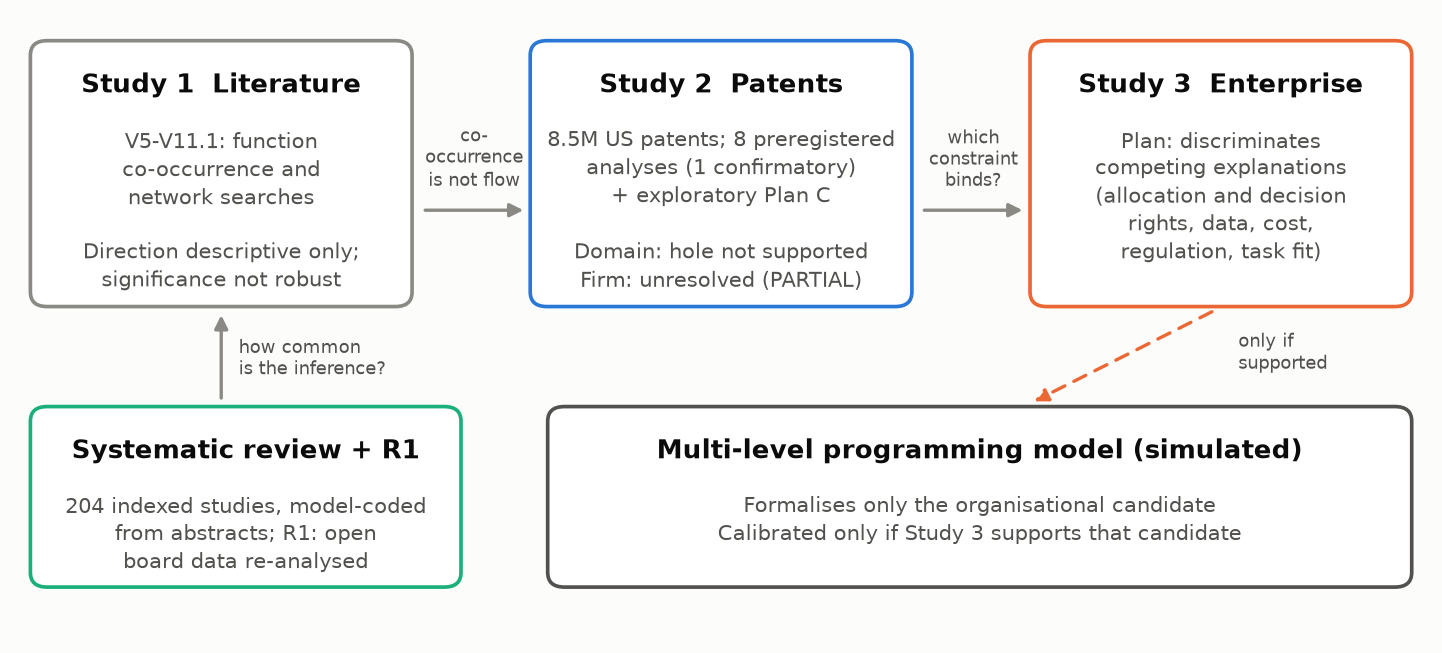
\includegraphics[width=\linewidth]{fig_research_design.png}
\caption[研究設計]{研究設計。研究一（文獻，V5--V11.1）顯示共現（co-occurrence）不等於流動；其方向僅屬描述性，且其顯著性並不穩健。研究二（美國專利；六項預先登錄〔preregistered〕的分析，其中一項為驗證性〔計畫 1〕、五項受資料啟發〔計畫 2--6，其中計畫 6 未通過其合格檢查〕，另加探索性的計畫 C；AI = CPC G06N；決策 = CPC G06Q10/04 與 G06Q10/06，而非整個 G06Q10）處理 RQ1 與 RQ2；圖中的概數對應 8,512,829 件發明專利（utility patents）。在領域層次，知識流動中的結構洞（structural hole）未獲支持（\texttt{HOLE\_\allowbreak NOT\_\allowbreak SUPPORTED}），但這並未證明結構洞不存在。在公司層次，此一問題仍未解決（判定為 \texttt{PARTIAL}）：在專利組合構成之外，仍存在顯著的專門型公司分隔，而混合型公司是否為其中介者（broker），無法以現有的虛無模型（null model）判定。因此，研究二未能釐清何種限制條件具有約束力。系統性文獻回顧（204 篇已索引研究，以模型依摘要層次編碼）與對公開董事會資料的 R1 重新分析，探討此一推論的普遍程度。研究三是一項尚無結果的規劃中企業研究，旨在區辨五種競爭解釋（competing explanations）。三層規劃模型（第 1 層：資源分配〔resource allocation〕；第 2 層：AI 架構與治理；第 3 層：人機配置）僅將組織層面的候選解釋形式化；其參數為模擬值，且僅在研究三支持該候選解釋時才會加以校準（虛線箭頭）。}
\label{zh:fig:research_design}
\end{figure}

\begin{table}[tbp]
\centering
\footnotesize
\setlength{\tabcolsep}{4pt}
\caption[研究與資料線概覽]{研究與資料線概覽。來源等級（provenance grade）的定義見第~\ref{zh:sec:design_prereg}~節：DIRECT；HIST.\ = HISTORICAL；USER = USER\_\allowbreak REPORTED；SIM.\ = SIMULATED。}
\label{zh:tab:front_overview}
\begin{tabular}{@{}p{0.16\linewidth}p{0.25\linewidth}p{0.16\linewidth}p{0.25\linewidth}p{0.09\linewidth}@{}}
\toprule
研究／資料線（狀態） & 資料 & 關係類型 & 主要檢定 & 等級 \tabularnewline
\midrule
\raggedright 研究一：功能矩陣（已完成） &
\raggedright 2,118 份來源文件；10 $\times$ 12 矩陣中 2,180 條文件層次的邊 &
\raggedright 共現（二模） &
\raggedright 四項虛無模型檢定並以 BH 偽發現率（FDR）校正；誤分類界限與模擬 &
\raggedright DIRECT \tabularnewline
\addlinespace
\raggedright 研究一：網路資料線 V6--V11.1（已完成） &
\raggedright 引用、共同著作與高階網路 &
\raggedright 引用篩檢與投影 &
\raggedright 搜尋 Burt 意義下的中介者；外部審查 &
\raggedright HIST.\ / USER \tabularnewline
\addlinespace
\raggedright 外部資料篩檢（已完成） &
\raggedright 六個公開來源（CORDIS H2020、GLEIF、OpenAlex、OCDS、SEC、PyPSA） &
\raggedright 隸屬、所有權、實體拓樸 &
\raggedright 獨立關係關卡與驗證關卡 &
\raggedright DIRECT \tabularnewline
\addlinespace
\raggedright 研究二：專利（已完成） &
\raggedright 8,512,829 件美國發明專利；AI = G06N；DEC = G06Q10/04 + G06Q10/06 &
\raggedright 有向申請人引用 &
\raggedright 六項預先登錄分析（計畫 1 為驗證性；計畫 2--6 受資料啟發；計畫 6 為 \texttt{INVALID\_\allowbreak NULL}）：總體檢定、CPC 矩陣、複製分析套組、兩個公司虛無模型、構念效度檢查；探索性的計畫 C &
\raggedright DIRECT \tabularnewline
\addlinespace
\raggedright 系統性文獻回顧與 R1（已完成） &
\raggedright 204 篇已索引研究（OpenAlex），由大型語言模型代理依摘要編碼；挪威董事會檔案（R1） &
\raggedright 依編碼：共現或隸屬；R1：二模隸屬 &
\raggedright 失效模式 F1--F4 與驗證 V 的盛行率；R1：保留隸屬結構的虛無模型 &
\raggedright DIRECT \tabularnewline
\addlinespace
\raggedright MLP 原型（示例） &
\raggedright 3 個流程；參數組 C／F／D；預算 3／5／7 &
\raggedright 無（模擬參數） &
\raggedright 精確逆向歸納 &
\raggedright SIM. \tabularnewline
\addlinespace
\raggedright 研究三：企業（計畫） &
\raggedright 一家或多家製造業公司的決策流程 &
\raggedright 規劃中的企業資料 &
\raggedright 以預先登錄的判定規則區辨競爭解釋 &
\raggedright -- \tabularnewline
\bottomrule
\end{tabular}
\end{table}

\section{選擇具流動效度的資料來源}
\label{zh:sec:design_sources}

在轉向專利之前，本研究以兩道關卡篩檢了六個公開的關係資料來源：獨立關係關卡與驗證關卡。CORDIS H2020（35,389 個專案；179,063 筆組織參與紀錄）產生的是共同成員關係，而非流動。在包含 49 次重複的保留度數二分交換虛無模型下，其 5 個可檢定的低限制度候選者之 $p$ = .41--.86，BH $q \geq .80$ \citep{benjamini1995controlling}；達顯著者為 0 個。GLEIF Level-2（663,449 筆關係紀錄，其中 481,247 筆為有效狀態）記錄的是法律上的合併（consolidation）關係。OpenAlex 回傳 8 筆著作，OCDS 回傳 0 條可驗證的採購者—供應者邊，而 PyPSA（8,786 個匯流排）描述的是實體電網。SEC 申報文件並未擷取，因為其存取需要真實的聯絡用 User-Agent。沒有任何來源同時通過兩道關卡：共同成員關係、所有權與實體拓樸皆非資訊流動。附錄表~\ref{zh:tab:app_sources} 報告完整的篩檢結果。

專利符合第~\ref{zh:sec:theory_holes}~節所述的要求。引用是有向流動 \citep{jaffe1993geographic}，CPC 分類是由審查員而非分析者指派的標籤，且資料涵蓋美國核准專利的母體，而非樣本。

\section{預先登錄紀錄與來源等級}
\label{zh:sec:design_prereg}

研究二以六項計畫進行預先登錄（preregistration）：計畫 1為總體領域檢定；計畫 2為在 CPC 格矩陣上進行的 V9 檢定組合；計畫 3為包含模組 P1--P10 的完整複製分析套組；計畫 4為保留專利組合的公司虛無模型（portfolio-preserving null）；計畫 5為構念效度（construct validity）檢查，係在計畫 1 的判定已知之後才擬定的後續分析（受資料啟發）；計畫 6為另依度數分層的公司虛無模型。探索性的計畫 C 則描述跨領域引用發生在哪裡。系統性文獻回顧的計畫書與 R1 重新分析計畫則另行凍結（附錄~\ref{zh:app:review}）。上述各項皆為專案儲存庫中的提交（commit）（為審查之故隱去識別碼；列於附錄~\ref{zh:app:prereg} 表~\ref{zh:tab:app_prereg} 與表~\ref{zh:tab:app_prereg_b}）。預先登錄的用意，是在觀察到結果之前固定分析計畫，以區分驗證性分析與探索性分析 \citep{nosek2018preregistration}。以下三項限定，界定了本研究的計畫在多大程度上符合此一標準。

第一，這些計畫是專案自有儲存庫中自行加註時間戳記的 git 提交，而非向第三方（例如開放科學架構〔Open Science Framework, OSF〕）所做的登錄；其時間戳記受作者控制，無法獨立驗證。第二，僅有計畫 1早於所有專利結果：它在下載任何專利資料之前即已凍結。計畫 2至計畫 6皆是在先前結果已知之後撰寫的，因此其研究問題受到資料的影響；只有其定義、虛無模型、判定規則、門檻、敏感度分析與停止規則（stop rule）是在計算之前固定的。計畫 4的動機來自計畫 3（模組 P5）的公司網路結果，並在計算其虛無模型重複樣本之前凍結；該虛無模型並非獨立於該結果而選定。第三，M06-P（專利適用之保留文件結構虛無模型）並不屬於計畫 2：它是在預先登錄的交換虛無模型失效之後，才於計畫 3（模組 P1）中凍結的（修訂 B1，第~\ref{zh:sec:study2_cells}~節）。因此，本研究將計畫 1視為驗證性的，而將計畫 2至計畫 6視為受資料影響的後續分析，其規則——而非其研究問題——是事先固定的。

偏離原計畫之處，以註明日期且不更動凍結文本的修訂（amendment）加以記錄（附錄表~\ref{zh:tab:app_amend}）。修訂 A1 在計算任何引用結果之前更正了一個 CPC 標籤的拼寫，並未改變設計中的任何內容。修訂 A2 記錄僅含申請人引用的設定實際上涵蓋 2013--2025 年的施引年份，並記錄計畫 1的 H3（一個以領域層次存在結構洞為條件的受讓人中介問題）因 H1 未獲支持而未執行；其後的公司分析（計畫 3，P5）係另行預先登錄，探討的是 RQ2，而 RQ2 並不以領域層次存在結構洞為前提。修訂 B1 記錄，預先登錄的格「核心」（core）——即在主要檢定、精確檢定與保留文件結構檢定（M06；調整後核心則為 M06-P）中皆為 $q \le .05$ 且方向相同，並且原始紀錄檢定亦為 $q \le .05$ 且方向相同的格；見第~\ref{zh:sec:study1_corpus}~節——在建構上即為空集合，因此以其餘三項檢定為依據的格結果屬於探索性。修訂 C1 在計畫 5 的初步結果已知之後、但在新增設定計算之前，為計畫 5 加入兩項更嚴格的構念設定。計畫 6 先以 2 次重複進行冒煙測試（smoke test），並將其檢定結果密封不讀；該測試已顯示合格檢查未通過，之後才進行完整執行。在系統性文獻回顧中，修訂 S1 在編碼之前擴大了裁決範圍；修訂 R1-A1 則在下載任何資料之前，加入原文章自身所用的快照。計畫 C 是一項探索性描述，說明跨領域引用發生在哪裡；它在計算之前即已凍結，但不檢定任何假設。研究一的資料效度再分析屬事後（post hoc）分析。

本研究中的每一個數字皆源自一份已記錄的結果檔，並具有三種來源等級（provenance grade）之一。DIRECT 數字係由凍結檔案重新計算或解析而得。HISTORICAL 數字報告於較早的專案紀錄中，其原始檔案已無法取得以重新驗證。USER\_\allowbreak REPORTED 數字則由研究者依據本地保存的檔案所報告。凡等級攸關之處，本研究皆予以註明；V6--V11.1 的網路結果屬 HISTORICAL 或 USER\_\allowbreak REPORTED，而 MLP 的輸出則為 SIMULATED。

\section{主張邊界}
\label{zh:sec:design_boundaries}

以下邊界規範本研究中的每一項主張：
\begin{enumerate}
\item[(i)] 在任何層次上，皆不主張已證實的結構洞。
\item[(ii)] 16 個 V9 偏低格，以及在 CPC 矩陣兩部分中皆偏低的 5 個專利格，均不稱為研究缺口。16 個 V9 格已撤回，不再作為 MLP 模型的依據。
\item[(iii)] 不主張任何因果效果。
\item[(iv)] MLP 的輸出為模擬結果，不反映任何真實公司。
\item[(v)] 「瓶頸在於組織」僅是數個候選解釋之一，並且是研究三的一項假說，而非研究結果。
\item[(vi)] 模型之間的一致性是可重現性的證據，而非人工信度的證據。
\item[(vii)] HISTORICAL 與 USER\_\allowbreak REPORTED 數據（V6--V11.1）皆如實標示。
\item[(viii)] 研究一偏低格的方向是一項描述，可能反映非隨機的編碼假象；它並非已證實的發現。
\end{enumerate}
全文中，「偏低」（depleted）與「偏高」（enriched）是相對於虛無模型對某一格所做的統計描述。它們本身並不構成領域之間存在分隔的證據。

% ======================================================================
% 第四章：研究結果（研究一：文獻證據；研究二：專利證據）
% 譯自 paper/en/studies.tex（英文稿第 4、5 節）。所有數字與英文稿及 raw_materials/experimental_log.md 一致。
% ======================================================================

\chapter{研究結果}
\label{zh:ch:results}

\section{研究一：文獻證據}
\label{zh:sec:study1}

研究一是結構洞（structural hole）前提最初被提出的研究脈絡。其專案版本標記為 V5--V11.1，僅用於將結果對應至專案紀錄：V5 建立文獻語料庫，V9 為 AI 家族 $\times$ 決策家族矩陣的凍結分析，V6--V11.1 則為網路分析脈絡。本研究連同 2026 年 11 月 18 日的資料效度再分析一併報告研究一；該再分析並未預先登錄（preregistration）。除標示為 HISTORICAL／USER\_REPORTED 者外（第~\ref{zh:sec:study1_network}~節），各數字的來源等級（provenance grade）皆為 DIRECT。

\subsection{語料庫、編碼與檢定設計}
\label{zh:sec:study1_corpus}

語料庫包含 2,118 份來源文件，其中 1,729 份完成剖析。剖析共產生 26,501 筆候選證據紀錄，其中 6,499 筆符合嚴格納入篩選條件。LLM 處理流程將每一個證據句歸入 10 個 AI 家族之一與 12 個決策家族之一，結果為一個含 120 格的二分網路（bipartite network）矩陣。在每份文件內去除重複後，得到 2,180 條文件層級的邊。120 格中有 104 格有觀察值；16 個零值格與下文所報告的 16 個偏低格（depleted cells）互不重疊。多數的邊（86.5\%）來自 AI 軌文件。對於邊際度數分別為 $k_a$ 與 $k_d$ 的 AI 家族 $a$ 與決策家族 $d$，期望次數為
\begin{equation}
E_{ad} = \frac{k_a\,k_d}{M}, \qquad M = 2{,}180 .
\label{zh:eq:s1_expected}
\end{equation}

每一格皆以四項檢定評估：
\begin{enumerate}
  \item 固定度數的端點重配蒙地卡羅（stub Monte Carlo）虛無模型（null model）（$R = 10{,}000$；種子 20260918）；
  \item 精確超幾何檢定（exact hypergeometric test）；
  \item 保留文件結構的文件內交換 MCMC（document-preserving swap null），於 V9 引擎中標記為 M06（5,000 個樣本，預燒期 43,600，抽稀間隔 4,360；種子 20260919）；
  \item 以未去除重複之紀錄進行的原始紀錄精確檢定（raw-record test）（$n = 3{,}125$）。
\end{enumerate}
Benjamini--Hochberg（BH）程序在 120 格內控制偽發現率（false discovery rate, FDR）\citep{benjamini1995controlling}。一格須同時符合下列條件，方納入凍結的\emph{核心格}（core）：在主要檢定、精確檢定與保留文件結構檢定中皆為 $q \le .05$ 且三者方向一致，另原始紀錄檢定亦須 $q \le .05$ 且方向相同。共有 32 格符合此規則，其中 16 格偏高、16 格偏低。「偏低」與「偏高」（enriched）是相對於上述虛無模型的統計描述，並非分隔（separation）的證據，本研究亦不將偏低格稱為缺口（第~\ref{zh:sec:design_boundaries}~節）。

以下兩項性質限定了其後的所有結果，包括專利類比分析（第~\ref{zh:sec:study2_cells}~節）：其一，精確檢定與原始紀錄檢定忽略文件內群聚（clustering）；其二，核心格結合了各檢定內的 BH 校正與相依檢定之間的一致性，因此並無單一明確定義的偽發現率，應解讀為一種保守的篩選（第~\ref{zh:sec:lim_inference}~節）。

\subsection{偏低格的方向與穩健性}
\label{zh:sec:study1_direction}

表~\ref{zh:tab:app_v9cells} 列出 16 個偏低格及其觀察次數。最極端者為 \texttt{PREDICTION\_\allowbreak RISK\_\allowbreak ESTIMATION}~$\times$ \texttt{HUMAN\_\allowbreak REVIEW\_\allowbreak ACCOUNTABILITY}，其 $O = 6$，而 $E = 44.9$。

\paragraph{計算穩健性。} 以獨立重新實作的精確檢定與原始紀錄檢定，可在 $|\Delta q| \le 6\times10^{-12}$ 的誤差內重現官方的 $q$ 值。32 格核心格的 Jaccard 重疊為 .94。在 20 個蒙地卡羅種子下，有 31 格在每一個種子下皆屬核心格，其中包括全部 16 個偏低格。其餘 2 個邊界格，恰為先前一次經人工校正之重新編碼所識別出的「一進一出」配對。

\paragraph{組成穩健性。} 在固定 AI 軌與決策軌文件組成的分軌分層虛無模型下，16/16 個偏低格與 16/16 個偏高格仍維持顯著且方向不變，故此型態並非 AI 軌文件居多所造成的假象。來自偏低核心格的紀錄通過嚴格篩選的比例高於來自其他格的紀錄（38\% 對 28\%）。

\paragraph{時間穩健性。} 圖~\ref{zh:fig:study1_direction} 將文件分為 2023 年（含）以前與 2024 年（含）以後兩期。全部 16 格在兩期中皆為偏低（16/16），且兩期之間的變化與置換虛無模型並無差異（$p = .86$）。因此，此一不足在兩期中方向相同。此判準僅涉及方向；變化不顯著僅代表缺乏變化的證據，而非穩定的證據。

\begin{figure}[tbp]
  \centering
  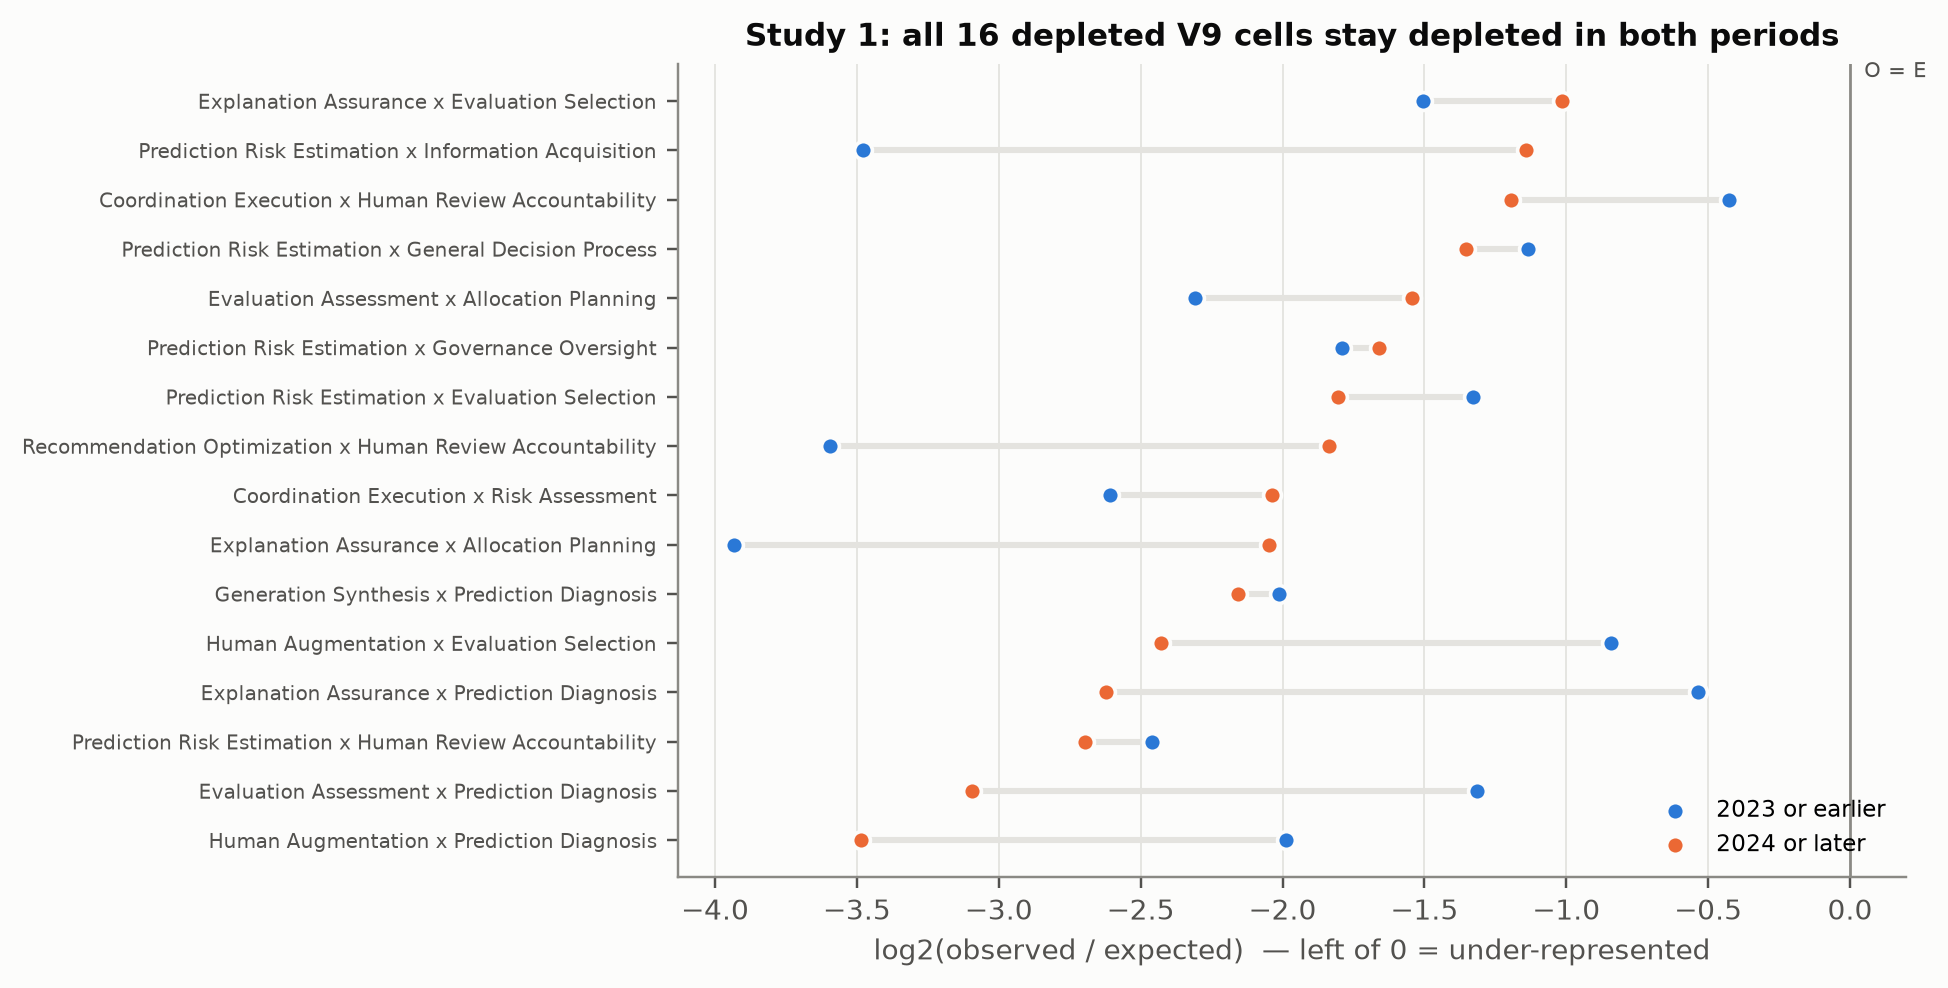
\includegraphics[width=\linewidth]{fig_study1_direction.png}
  \caption{研究一：16 個 V9 偏低格各自的 $\log_2(O/E)$，分別以 2023 年（含）以前（藍色）與 2024 年（含）以後（橙色）的文件計算。垂直線標示 $O = E$。各期的期望次數係以該期自身的邊際重新計算，故各期數值無法直接與合併計算的 O/E 比較（最極端格的合併值為 $O = 6$，$E = 44.9$）。此方向可能反映非隨機的編碼假象（第~\ref{zh:sec:study1_reliability}~節）。此為偏低格，而非缺口。DIRECT。}
  \label{zh:fig:study1_direction}
\end{figure}

\paragraph{三角檢證的限度。} 一旦編碼工具改變，方向的穩固程度便隨之降低：
\begin{itemize}
  \item 在關鍵詞（第一階段）編碼下，13/16 個偏低格維持相同方向。
  \item 同詞兩端共用（same-term self-pairing）膨脹了最強的偏高格（prediction $\times$ prediction）。該格中有 33\% 的紀錄在兩端配對同一詞彙（例如「forecasting」）。移除這些紀錄後，有 2 個與預測相關的偏低格退出核心格。
  \item 規則式關鍵詞矩陣移除 741 筆同詞紀錄，剩下 1,431 條文件邊。在此矩陣中，13/16 個偏低格維持相同方向，6 格顯著，0 格呈顯著反轉，但僅有 7 格進入四項檢定的核心格。
\end{itemize}
因此，偏低的方向對種子、來源軌與時期皆具穩健性，對關鍵詞編碼與移除同詞紀錄亦大致穩健。相對地，顯著核心格的組成則取決於句子的編碼方式。表~\ref{zh:tab:app_s1robust} 彙整所有穩健性檢查。

\subsection{測量信度與誤分類}
\label{zh:sec:study1_reliability}

表~\ref{zh:tab:reliability} 報告 AI 標籤與決策標籤經機遇校正的一致性（Cohen's $\kappa$；\citealp{cohen1960coefficient}）。

\begin{table}[tbp]
  \centering
  \small
  \caption{研究一標籤的編碼信度（Cohen's $\kappa$）。模型與模型之間的一致性僅顯示工具具可重現性，並非人工的評分者間信度（inter-rater reliability）。人工與人工之間的估計僅根據 $n = 20$ 筆紀錄，因此並不精確。DIRECT。}
  \label{zh:tab:reliability}
  \begin{tabular}{p{0.62\linewidth}rr}
    \toprule
    比較 & AI $\kappa$ & 決策 $\kappa$ \\
    \midrule
    人工 vs 人工（$n = 20$） & 0.05 & 0.14 \\
    處理流程 LLM（qwen）vs 第一位人工編碼者（$n = 50$） & 0.27 & 0.12 \\
    處理流程 LLM 再測（143 個標籤端） & 0.64 & 0.63 \\
    理論合併分類（7$\times$6），人工 vs 人工 & 0.08 & 0.16 \\
    兩個 Claude 模型，盲測，編碼手冊 v2（250 筆紀錄）：Sonnet vs Haiku$^{a}$ & 0.72 (0.87) & 0.56 (0.82) \\
    Claude（編碼手冊 v2）vs 協調後的人工答案（$n = 20$） & 0.45 & 0.70--0.76 \\
    處理流程 qwen vs 協調後的人工答案 & 0.11 & 0.29 \\
    \bottomrule
  \end{tabular}

  \smallskip
  \raggedright\footnotesize $^{a}$括號內為兩個模型皆有編碼之標籤端之間的一致性。
\end{table}

人工與人工之間的一致性極低，且僅基於 20 筆紀錄；改用較粗略的分類亦未見改善。處理流程在再測時穩定，但與人工編碼的一致性薄弱。兩個 Claude 模型之間的一致性較高，這顯示的是程序具可重現性，而非具可靠性。修訂後的編碼手冊也改變了被編碼的內容：在編碼手冊 v2 下，42--64\% 的證據句未陳述明確的決策功能，而處理流程的比例為 18\%；且僅約 9\% 的矩陣紀錄被兩位新編碼者重現於同一格中。

\paragraph{解析界限及其限度。} 令 $T$ 為一格在無誤編碼下的次數，$e_{\mathrm{AI}}$ 與 $e_{\mathrm{Dec}}$ 為兩個標籤的非差異性（隨機）誤差率。則
\begin{equation}
\frac{O^{\mathrm{obs}}}{E} - 1 = (1 - e_{\mathrm{AI}})(1 - e_{\mathrm{Dec}})\left(\frac{T}{E} - 1\right).
\label{zh:eq:attenuation}
\end{equation}
由於正確率乘積至多為 1，隨機誤差只會削弱偏低，而不會製造偏低。然而，此界限並不能保護方向，原因有二。

第一，此界限僅涵蓋非差異性誤分類（non-differential misclassification），而已記錄的兩項誤差來源並非隨機。同詞兩端共用膨脹了 prediction $\times$ prediction 格。在式~\eqref{zh:eq:s1_expected} 下，膨脹某一格會提高其所在列與欄的邊際，從而提高同列與同欄其他格的期望次數，使其 O/E 下降；因此，在固定邊際的矩陣中，編碼可能製造出偏低。本研究自身的移除證據限制了此一機制。在不含 741 筆同詞紀錄的情況下，13/16 個偏低格維持其方向，且無一呈顯著反轉；而自被膨脹的格中移除同詞配對紀錄，僅使 2 個偏低格退出核心格（第~\ref{zh:sec:study1_direction}~節）。因此，同詞兩端共用並非此型態的主要驅動因素。模型推論的標籤是第二個非隨機來源，且尚未經過檢驗：若模型將特定類型的句子導向特定家族，便會以有規律的方式在格與格之間移動紀錄。

第二，隨機誤差模型與資料並不相符。以最極端格而言，即使採用 95\% 上界，也需要正確率乘積至少為 0.71，而人工稽核所隱含的值約為 0.07。這指向非隨機誤差，或指向稽核規模過小而無法估計正確率；觀察到的幅度不應被解讀為人工編碼資料將會呈現的結果。

\paragraph{模擬。} 表~\ref{zh:tab:misclass} 在六種誤分類情境下重建矩陣，並重新執行 BH 精確檢定。當以任一人工編碼作為真值時，仍維持顯著之偏低格數的中位數為 0，儘管分別有 11 與 12 格維持其方向。僅最輕微的隨機誤差情境與 Claude 共識情境維持非零的中位數（7 與 4）。沒有任何情境產生虛假的偏低格，但模擬的誤差皆為隨機誤差，故此結果對非隨機誤差無法提供任何資訊。由於兩位人工編碼者在 20 筆紀錄上大多不一致，「作為真值」的情境屬於壓力測試，而非經校準的誤差模型。

\begin{table}[tbp]
  \centering
  \small
  \caption{16 個偏低格的誤分類模擬：每種情境執行 300 次。每次皆重建矩陣並重新執行 BH 精確檢定。表中數值為格數的中位數（第 5--95 百分位數）。所有模擬誤差皆為隨機誤差；「作為真值」的情境為壓力測試。沒有任何情境產生虛假的偏低格。DIRECT。}
  \label{zh:tab:misclass}
  \begin{tabular}{lll}
    \toprule
    情境 & 仍顯著 & 仍偏低 \\
    \midrule
    第一位人工編碼者作為真值 & 0 (0--1) & 11 (8--13) \\
    協調後的人工編碼作為真值 & 0 (0--1) & 12 (10--14) \\
    20\% 隨機誤差 + 20\% 刪除 & 7 (5--10) & 16 (15--16) \\
    40\% 隨機誤差 + 20\% 刪除 & 0 (0--1) & 14 (12--16) \\
    60\% 隨機誤差 + 20\% 刪除 & 0 (0--0) & 10 (7--13) \\
    Claude 共識（編碼手冊 v2）作為真值 & 4 (3--6) & 14 (12--15) \\
    \bottomrule
  \end{tabular}
\end{table}

2026 年 11 月 18 日的再分析記錄了四項判定：
\begin{itemize}
  \item 方向性的低整合（under-integration）：\texttt{DEFENSIBLE}；
  \item 「16 個統計上穩健的偏低配對」：依現行測量為 \texttt{NOT DEFENSIBLE}；
  \item Burt 結構洞：\texttt{STOP}，因此中介者（broker）搜尋予以終止；
  \item 研究缺口：\texttt{NOT SUPPORTED}。
\end{itemize}
本研究對第一項判定加以限定。此方向通過了本研究所能執行的每一項檢查，且同詞兩端共用無法解釋其大部分，但模型推論的標籤仍可能形塑了此方向。這是一個描述性、未經確認的型態，而「defensible」（可辯護）的意義僅止於此。

\subsection{網路分析脈絡 V6--V11.1 與 Gap Validity}
\label{zh:sec:study1_network}

研究一的歷次版本在引用網路、共同作者網路與高階網路中搜尋 Burt 式中介者（表~\ref{zh:tab:network_lines}）。根據這些 HISTORICAL／USER\_REPORTED 紀錄，沒有任何一條脈絡確認出中介者。V10.1 對 8 組候選配對的外部審查否證了其中 6 組，另有 2 組未能判定。V11.1 的身分與同儕驗證否決了 4 名候選者中的 3 名，並認定第 4 名的證據不足。

\begin{table}[tbp]
  \centering
  \small
  \caption{V6--V11.1 對 Burt 式中介者的網路搜尋。所有列皆為 HISTORICAL／USER\_REPORTED：取自先前的專案紀錄或由研究者報告，原始檔案未經重新驗證。}
  \label{zh:tab:network_lines}
  \setlength{\tabcolsep}{4pt}
  \begin{tabular}{l p{0.17\linewidth} p{0.33\linewidth} p{0.17\linewidth} l}
    \toprule
    版本 & 脈絡 & 規模 & 結果 & 等級 \\
    \midrule
    V6 & 引用 SNA & 458 條線索；13 名候選者 & 0 名確認 & HIST./USER \\
    V7 & 作者 SNA & 446 篇著作；8 名跨領域作者；2 名焦點候選者 & 0 名確認 & HIST./USER \\
    V8 & 引用擴充 & 1,111 篇施引著作；5,592 筆參考文獻 & 未確認 & HIST./USER \\
    V9 & 引用脈絡 & 3,983 篇探索著作 + 3,897 篇確認著作（共 7,880 篇） & 無確認的 Burt 結果 & HIST./USER \\
    V10 & 高階網路 & 14 名探索性候選者 $\rightarrow$ 8 組配對／7 名中介者 & 僅屬探索性 & HIST./USER \\
    V10.1 & 外部審查 & 8 組候選配對 & 6 組否證、2 組未定、0 組確認 & HIST./USER \\
    V11 & 共同作者 SNA & 26,443 名 V9 作者；30,140 名合併後作者 & 0 名確認 & HIST./USER \\
    V11.1 & 外部身分／同儕驗證 & 95 次 OpenAlex 查詢；檢視 7,880 篇著作；4 名候選者 & 3 名否決、1 名證據不足、0 名確認 & HIST./USER \\
    \bottomrule
  \end{tabular}

  \smallskip
  \raggedright\footnotesize SNA = 社會網路分析（social network analysis）。HIST./USER = HISTORICAL／USER\_REPORTED。
\end{table}

各脈絡所用的關係能承載的內容並不相同。共同作者脈絡（V7、V11）與高階脈絡（V10）建立在投影之上。共同作者網路是作者--著作隸屬資料的單模投影（one-mode projection）\citep{newman2001scientific}，因此共同發表一篇論文並非有方向的流動（flow）；即使資料完美無誤，這些脈絡也無法承載 Burt 的構念（第~\ref{zh:sec:theory_cooccurrence}~節）。引用脈絡（V6、V8、V9）則不同：引用原則上能承載有方向的流動，這也是研究二採用引用的原因。這些脈絡之所以失敗，是基於資料與設計上的理由：它們在文獻樣本中篩選候選中介者，而非針對經校準的虛無模型檢定群體層級的流動。以中心性為基礎的篩選，例如通過某一節點之最短路徑的比例 \citep{freeman1977set}，並不能確立中介（brokerage）；中介需要在具有群體成員身分的行動者之間存在有方向的開放二步路徑 \citep{gould1989structures}，而 Burt 所述的效益則建立在非冗餘的真實聯繫之上 \citep{burt1992structural}。

補充診斷 Gap Validity（DIRECT）記錄：全部 16 個偏低格在二分家族網路中皆有替代路徑（16/16），且網路限制度（Burt constraint）的間接項為零。兩者皆非實證證據：間接項為零對任何嚴格二分圖而言皆為恆等式（第~\ref{zh:sec:theory_cooccurrence}~節），而在 120 格中有 104 格有觀察值的情況下，替代路徑幾乎必然存在。此診斷僅明確指出：偏低格並不代表斷裂。

因此，研究一支持一項描述性主張：在此文獻中，依現行編碼，16 個偏低配對的共現（co-occurrence）頻率低於其邊際所隱含的水準，且在兩期中方向相同。此型態究竟屬於文獻本身或源自編碼，無法以這些資料判定。檢驗此前提需要有方向的流動，而這正是研究二所提供的。

% ======================================================================

\section{研究二：專利證據}
\label{zh:sec:study2}

研究二以有方向的知識流動（knowledge flow）檢驗此前提：即美國發明專利（utility patents）之間的申請人引用（applicant citation），並以審查員指派的 CPC 分類作為群體標籤。本研究是在六個公開的關係型資料來源未能通過流動效度關卡之後，才選定專利資料（第~\ref{zh:sec:design_sources}~節；表~\ref{zh:tab:app_sources}）。各項分析遵循第~\ref{zh:sec:design_prereg}~節所述的四份預先登錄計畫（表~\ref{zh:tab:app_prereg}）：這些計畫為自行加上時間戳記的提交（commit），其中僅計畫 1 早於所有專利結果，因此對於計畫 2--4，本研究主張的是其規則係事先固定，而非其研究問題係事先固定。各項偏離均以註明日期的修訂（amendment）記錄（表~\ref{zh:tab:app_amend}）。本節所有結果皆為 DIRECT。

\subsection{資料與整體檢定}
\label{zh:sec:study2_aggregate}

\paragraph{資料。} 本研究使用 USPTO PatentsView 的 \texttt{pvgpatdis} 資料表，下載日期為 2026 年 11 月 18 日 \citep{uspto2026patentsview}：包括 1976--2025 年核准的 8,512,829 件發明專利，以及 152,631,929 列引用資料；其中 87,414,291 列屬於分析範圍（施引年份 2010--2025），而這些引用中又有 63,083,371 列為申請人引用。引用被用作知識流動的代理指標 \citep{jaffe1993geographic}。由審查員加入的引用（examiner citation）可能無法反映發明人所知，因此主要設定僅使用申請人引用 \citep{alcacer2006patent}。由於 PatentsView 在 2013 年以前將非審查員引用標示為「cited by other」，此設定實際上涵蓋施引年份 2013--2025。

各群體採用核准年份 2010--2025：
\begin{itemize}
  \item AI（CPC \texttt{G06N}）：94,929 件專利；
  \item DEC（\texttt{G06Q10/04}，預測與最佳化；加上 \texttt{G06Q10/06}，資源、工作流程、管理與決策分析）：37,501 件；
  \item BRIDGE（兩者皆屬）：5,316 件；
  \item 其他商業方法專利（BIZ-OTHER；\texttt{G06Q} 但不含 \texttt{G06Q10}）：150,170 件。
\end{itemize}
跨群體計數排除橋接（BRIDGE）專利。

\paragraph{DEC 的構念效度。} \texttt{G06Q10/04}（預測與最佳化）在方法上與機器學習重疊，因此 AI--DEC 過度連結（over-connection）的一部分可能近乎機械性：兩個分類部分描述的是相同的技術。因此，此檢定所測量的是專利分類之間的技術鄰近性，而非 AI 融入管理決策的程度。構念效度（construct validity）仍未經檢驗。敏感度檢查 s2 將 DEC 擴大至整個 \texttt{G06Q10}，使強度 OE（見下文式~\eqref{zh:eq:oe}）由 3.05 降至 2.59，但判定不變（表~\ref{zh:tab:aggregate}）；然而 s2 仍包含 \texttt{/04}，因此只是稀釋而非隔離此一重疊。僅以 DEC = \texttt{G06Q10/06} 進行的分析，以及粒度相符的 H1a 參照集（見下文），本研究均未執行；兩者是未來研究最優先的穩健性檢查。領域層級的判定適用於此處所定義的 \texttt{G06N} 對 \texttt{G06Q10/04} + \texttt{/06}。

\paragraph{統計量。} 引用依 $s = $（施引專利核准年份，被引專利核准年份）分層。在每一層中，$\mathrm{out}_A(s)$ 為群體 $A$ 專利所做出的引用數，$\mathrm{in}_B(s)$ 為群體 $B$ 專利所獲得的引用數，$M(s)$ 為總數。時間分層的組態期望值（configuration expectation）為
\begin{equation}
E(A\!\rightarrow\!B) = \sum_{s} \frac{\mathrm{out}_A(s)\,\mathrm{in}_B(s)}{M(s)} ,
\label{zh:eq:patent_expected}
\end{equation}
而對稱的觀察對期望強度 OE 為
\begin{equation}
\mathrm{OE}(A,B) = \frac{O(A\!\rightarrow\!B) + O(B\!\rightarrow\!A)}{E(A\!\rightarrow\!B) + E(B\!\rightarrow\!A)} .
\label{zh:eq:oe}
\end{equation}

\paragraph{為何採用相對檢定。} 由於引用行為具有領域在地性，若採用絕對判準「$\mathrm{OE} < 1$」，幾乎任何一對領域都會被標記（第~\ref{zh:sec:theory_domains}~節）。在使用真實資料之前執行的合成校準顯示了這一點：在未植入結構洞時，$\mathrm{OE} = 0.388$，但檢定正確地回傳 \texttt{HOLE\_\allowbreak NOT\_\allowbreak SUPPORTED}；而在跨群體引用受到 30\% 或 50\% 抑制時，檢定能偵測出結構洞（表~\ref{zh:tab:app_oeyear}）。此生成器相當簡單（領域在地的引用加上植入的抑制），其無結構洞的基準線接近參照最低四分位數，而真實 OE 則遠高於此；此校準顯示的是從低基準線出發的偵測能力，而非在真實基準線下的檢定力。預先登錄的假說皆為相對假說：
\begin{itemize}
  \item \textbf{H1a：}$\mathrm{OE}(\mathrm{AI},\mathrm{DEC})$ 同時落在 $\{\mathrm{OE}(\mathrm{AI},X)\}$ 與 $\{\mathrm{OE}(\mathrm{DEC},X)\}$ 的最低四分位數 $Q_1$ 之內。參照集為 \texttt{G06}、\texttt{G16} 與 \texttt{H04} 中至少有 2,000 件專利的 179 個 CPC 大組（main group）。
  \item \textbf{H1b：}比值 $\mathrm{OE}(\mathrm{AI},\mathrm{DEC}) / \mathrm{OE}(\mathrm{AI},\mathrm{BIZ\text{-}OTHER})$ 小於 1，且其 95\% 信賴上界小於 1。
\end{itemize}
H1a 並未匹配粒度：DEC 由兩個 CPC 小組（subgroup）構成，而參照對象則為大組。範圍窄且同質的群體可能比範圍廣的群體呈現較高的 OE，因此 H1a 的百分位數可能偏向過度連結。本研究未計算小組層級的參照集。

\paragraph{結果。} 在主要設定下，$O = 30{,}843$，$E = 10{,}112$，得 $\mathrm{OE}(\mathrm{AI},\mathrm{DEC}) = 3.05$（95\% CI 2.94--3.17；以施引專利為群集的 Poisson 群集拔靴法，2,000 次重複）。兩個方向皆呈過度代表：AI$\rightarrow$DEC 為 $O = 21{,}820$、$E = 6{,}686$（O/E 3.26），DEC$\rightarrow$AI 為 $O = 9{,}023$、$E = 3{,}426$（O/E 2.63）。H1a 不成立：OE(AI,DEC) 高於 97.8\% 的 OE(AI,$X$) 值與 92.2\% 的 OE(DEC,$X$) 值，而最低四分位數門檻分別為 0.787（AI 側）與 0.502（DEC 側），中位數分別為 1.240 與 1.095。H1b 不成立：比值為 1.69（95\% CI 1.60--1.77），儘管比較配對本身亦呈過度連結（$\mathrm{OE}(\mathrm{AI},\mathrm{BIZ\text{-}OTHER}) = 1.809$）。預先登錄的判定為 \texttt{HOLE\_\allowbreak NOT\_\allowbreak SUPPORTED}。

全部六項預先登錄的敏感度分析（sensitivity analysis）設定皆與此判定一致（0/6 不一致；表~\ref{zh:tab:aggregate}、圖~\ref{zh:fig:patent_sensitivity}），因此依預先登錄的規則，此判定並不脆弱。OE 的範圍介於 2.59（s2，DEC 擴大至整個 \texttt{G06Q10}）至 4.25（s6，橋接專利於兩側皆計入）之間。

\begin{table}[tbp]
  \centering
  \caption{整體檢定：主要設定與六項預先登錄的敏感度設定。「相對 BIZ 比值」為 OE(AI,DEC)/OE(AI,BIZ-OTHER) 及其 95\% 拔靴法 CI。「百分位數」為 179 個參照值 OE(AI,$X$)／OE(DEC,$X$) 中被 OE(AI,DEC) 超過的比例。NOT\_SUPPORTED 為 HOLE\_NOT\_SUPPORTED 的縮寫。DIRECT。}
  \label{zh:tab:aggregate}
  \footnotesize
  \setlength{\tabcolsep}{4pt}
  \begin{tabular}{p{0.26\linewidth}rlll}
    \toprule
    設定 & OE(AI,DEC) & 相對 BIZ 比值（95\% CI） & 百分位數 AI／DEC & 判定 \\
    \midrule
    主要設定 & 3.05 & 1.69 (1.60--1.77) & 97.8\% / 92.2\% & \texttt{NOT\_\allowbreak SUPPORTED} \\
    s1 所有引用類別 & 3.00 & 1.65 (1.55--1.75) & 98.9\% / 92.7\% & \texttt{NOT\_\allowbreak SUPPORTED} \\
    s2 DEC = 整個 \texttt{G06Q10} & 2.59 & 1.43 (1.38--1.49) & 95.5\% / 89.9\% & \texttt{NOT\_\allowbreak SUPPORTED} \\
    s3 擴大 AI（+\texttt{G06F18}、\texttt{G06V10/70}） & 2.69 & 1.56 (1.50--1.63) & 94.4\% / 86.6\% & \texttt{NOT\_\allowbreak SUPPORTED} \\
    s4 僅限發明資訊（inventive）分類碼 & 3.00 & 1.62 (1.54--1.70) & 97.7\% / 94.5\% & \texttt{NOT\_\allowbreak SUPPORTED} \\
    s5 施引年份 2015+ & 3.04 & 1.69 (1.61--1.78) & 98.2\% / 92.9\% & \texttt{NOT\_\allowbreak SUPPORTED} \\
    s6 橋接專利計入兩側 & 4.25 & 2.35 (2.23--2.47) & 100\% / 99.4\% & \texttt{NOT\_\allowbreak SUPPORTED} \\
    \bottomrule
  \end{tabular}
\end{table}

\begin{figure}[tbp]
  \centering
  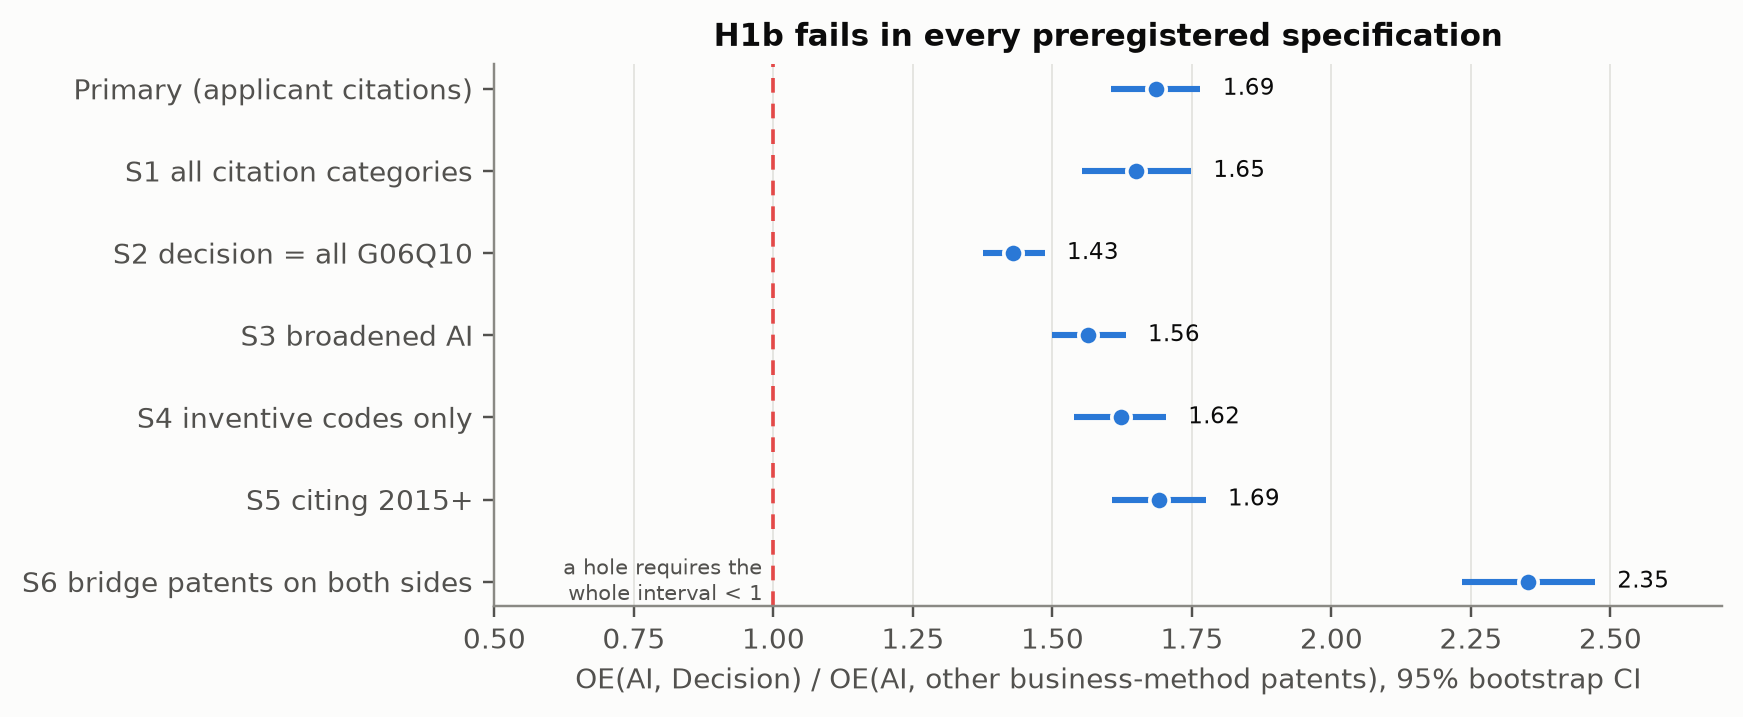
\includegraphics[width=\linewidth]{fig_patent_sensitivity.png}
  \caption{主要設定與六項敏感度設定下的 H1b 比值 OE(AI,DEC)/OE(AI,BIZ-OTHER) 及其 95\% CI。結構洞的成立要求整個區間皆落在 1 的虛線之下；每個區間皆位於其上。H1a 的百分位數見表~\ref{zh:tab:aggregate}。}
  \label{zh:fig:patent_sensitivity}
\end{figure}

\paragraph{趨勢（H2）。} 圖~\ref{zh:fig:patent_trend} 依施引年份繪出 OE(AI,DEC)。其值由 2013 年的 3.90 降至 2025 年的 2.34，加權最小平方斜率為每年 $-0.097$（95\% CI $-0.130$ 至 $-0.065$）。最近三年的 OE 為 2.69，而 DEC 側參照中位數為 1.095（AI 側為 1.240）。預先登錄的規則在斜率的 95\% CI 包含 0 或位於 0 以下時，將趨勢標記為 \texttt{PERSISTENT}，此處即屬後者。此規則原為結構洞情形而撰寫，在該情形中「收斂」意指 OE 朝參照值上升；套用於過度連結時，此標籤僅表示 OE 並未依該意義收斂，而非表示過度連結是穩定的。過度連結正在下降，但仍為 DEC 側參照中位數的兩倍以上。各年數值見表~\ref{zh:tab:app_oeyear}。

\begin{figure}[tbp]
  \centering
  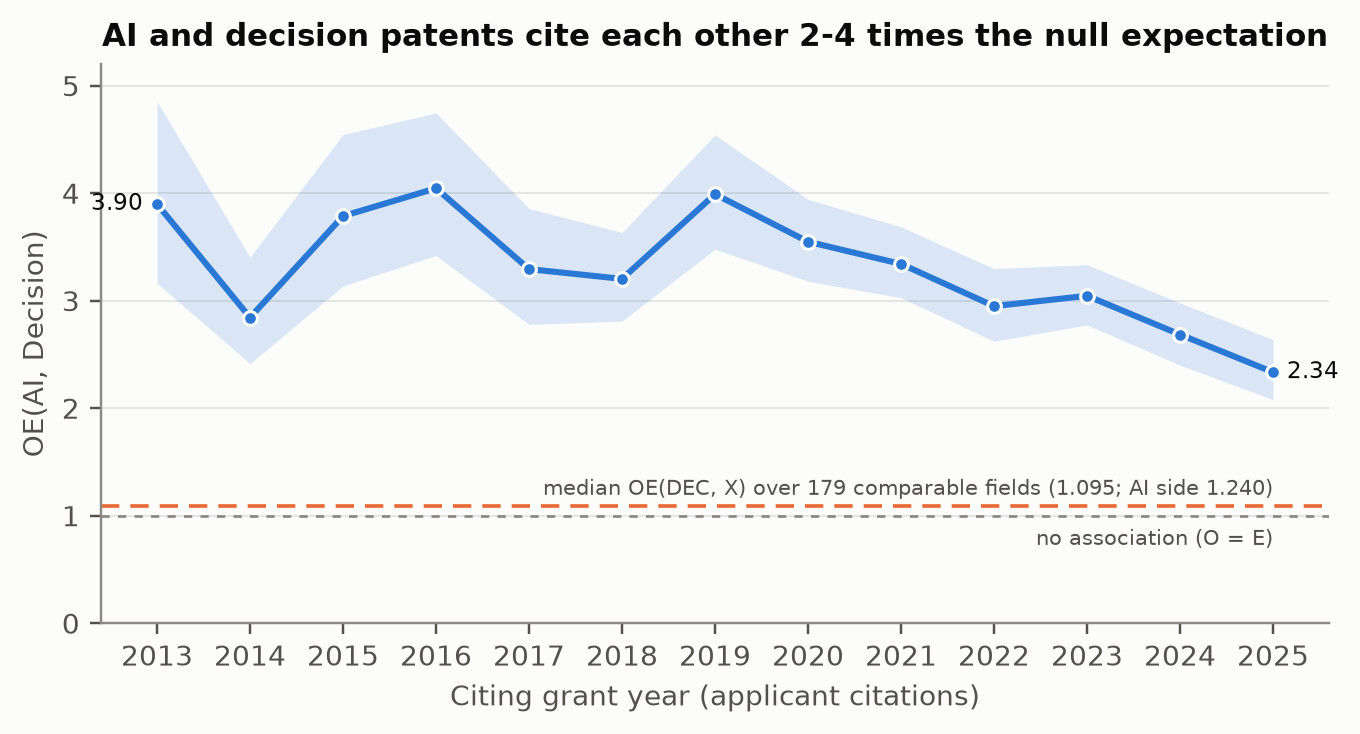
\includegraphics[width=\linewidth]{fig_patent_trend.png}
  \caption{2013--2025 年依施引專利核准年份計算的 OE(AI,DEC)，附 95\% CI 帶（僅申請人引用）。虛線為 DEC 側參照中位數，即 179 個可比較領域之 OE(DEC,$X$) 的中位數（1.095；AI 側中位數為 1.240），點線為 $O = E$。預先登錄標籤：\texttt{PERSISTENT}（斜率 CI 未高於 0；第~\ref{zh:sec:study2_aggregate}~節），儘管此序列呈下降趨勢。}
  \label{zh:fig:patent_trend}
\end{figure}

就 RQ1 而言，在此處的操作化定義下（\texttt{G06N} 對 \texttt{G06Q10/04} + \texttt{/06}），證據並不支持 AI 與決策技術之間的知識流動存在結構洞。這是在預先登錄規則下未能支持結構洞，而非證明不存在任何分隔；且過度連結的大小也不是組織整合程度的測量。

\subsection{CPC 矩陣上的 V9 檢定組與 M06-P 虛無模型}
\label{zh:sec:study2_cells}

預先登錄 2 將研究一的檢定組套用於功能矩陣的專利類比版本。此矩陣共有 42 格：
\begin{itemize}
  \item 6 個 AI 方法列：\texttt{G06N3}（神經網路）、\texttt{G06N5}（知識本位）、\texttt{G06N7}（機率／模糊）、\texttt{G06N10}（量子）、\texttt{G06N20}（機器學習）與 \texttt{G06N\_\allowbreak OTHER}；
  \item 7 個決策功能欄：FORECAST\_\allowbreak OPTIMISE（\texttt{G06Q10/04}）、RESOURCE\_\allowbreak SCHEDULING（\texttt{/0631}）、WORKFLOW（\texttt{/0633}）、RISK（\texttt{/0635}）、STRATEGY（\texttt{/0637}）、PERFORMANCE（\texttt{/0639}）與 MGMT\_\allowbreak GENERAL（其他 \texttt{/06}）。
\end{itemize}
所用引擎為 V9 引擎的位元組完全相同之複本（SHA-256 \texttt{09c3d60c\ldots bc33}）。此檢定組在三個部分上執行：
\begin{itemize}
  \item A 部分（Part A），共同分類：5,316 件專利與 14,573 條邊；
  \item B 部分（Part B），純 AI 專利與純 DEC 專利之間的申請人引用：30,843 筆引用與 66,056 條邊；
  \item 含所有引用類別的 B 部分：38,252 筆引用與 80,849 條邊。
\end{itemize}
由於 B 部分的 66,056 條邊來自 30,843 筆引用，第~\ref{zh:sec:study1_corpus}~節所述的群聚限制在此同樣適用。

\paragraph{退化的虛無模型及其替代。} 預先登錄的保留文件結構交換（M06）在 21,843,600 次提議的交換中接受了 0 次。原因是結構性的：每件專利貢獻其分類碼完整的列 $\times$ 欄乘積，因此每一個候選交換所指向的邊都已存在。預先登錄的核心格因而在建構上必然為空，對資料不提供任何資訊（修訂 B1，表~\ref{zh:tab:app_amend}）。其替代者為 M06-P（專利適用之保留文件結構虛無模型），它在（$|$列$|$, $|$欄$|$）分層內於文件之間置換欄集合，從而同時保留兩側邊際與每份文件的區塊結構（5,000 個樣本）。M06-P 是在 M06 失敗之後、且在三項檢定的格層級結果已知之後才設計的。它是對預先登錄 2 的有紀錄偏離，並在計算之前被凍結為預先登錄 3 的模組 P1；下文 M06-P 的結果即為 P1 的結果。M06-P 沒有獨立的型一誤差校準。

\paragraph{結果。} \emph{調整後完整核心}（adapted full core），即以 M06-P 取代 M06 的研究一核心規則，在 A 部分包含 8 個偏低格與 7 個偏高格，在 B 部分包含 9 個偏低格與 8 個偏高格，在含所有類別的 B 部分則為 8 與 8。各檢定（主要／精確／原始／M06-P）中 $q \le .05$ 的格數，在 A 部分為 20 / 20 / 29 / 22，在 B 部分為 22 / 22 / 27 / 25。表~\ref{zh:tab:cells_both} 列出在三項檢定一致（主要 + 精確 + 原始）下，於 A 與 B 皆偏低的五格，以及於兩者皆偏高的四格。依修訂 B1，三項檢定的結果屬探索性。圖~\ref{zh:fig:cpc_heatmap} 呈現完整矩陣。

\begin{table}[tbp]
  \centering
  \small
  \caption{在共同分類（A 部分）與引用流動（B 部分）中同方向偏離的 CPC 格。數值為 O/E，括號內為觀察／期望次數。偏低列：調整後完整核心（M06-P；預先登錄 3，模組 P1）與三項檢定一致給出相同的集合。偏高列依據三項檢定一致（主要 + 精確 + 原始），屬探索性（修訂 B1）。\texttt{G06N10}~$\times$~PERFORMANCE 屬小樣本（B 部分期望次數低於 10；A 部分整個量子列僅有 74 條邊）。此為偏低格，而非缺口。DIRECT。}
  \label{zh:tab:cells_both}
  \begin{tabular}{llll}
    \toprule
    AI 方法 & 決策功能 & A 部分 & B 部分 \\
    \midrule
    \multicolumn{4}{l}{\emph{A 與 B 皆偏低}} \\
    \texttt{G06N3} & RISK & 0.78 (171 / 219.5) & 0.70 (1,050 / 1,510.6) \\
    \texttt{G06N5} & RISK & 0.87 (255 / 291.9) & 0.85 (2,008 / 2,366.6) \\
    \texttt{G06N3} & MGMT\_\allowbreak GENERAL & 0.87 (497 / 572.7) & 0.95 (4,189 / 4,414.8) \\
    \texttt{G06N20} & FORECAST\_\allowbreak OPTIMISE & 0.89 (994 / 1,120.9) & 0.93 (2,255 / 2,425.9) \\
    \texttt{G06N10} & PERFORMANCE & 0.08 (1 / 12.0) & 0 (0 / 8.9) \\
    \midrule
    \multicolumn{4}{l}{\emph{A 與 B 皆偏高（主要 + 精確 + 原始；探索性）}} \\
    \texttt{G06N20} & RISK & 1.18 & 1.33 \\
    \texttt{G06N3} & FORECAST\_\allowbreak OPTIMISE & 1.09 & 1.17 \\
    \texttt{G06N5} & MGMT\_\allowbreak GENERAL & 1.16 & 1.06 \\
    \texttt{G06N7} & PERFORMANCE$^{a}$ & 1.15 & 1.16 \\
    \bottomrule
  \end{tabular}

  \smallskip
  \raggedright\footnotesize $^{a}$僅於 B 部分屬調整後完整核心（A 部分 M06-P $q = .93$）。
\end{table}

\begin{figure}[tbp]
  \centering
  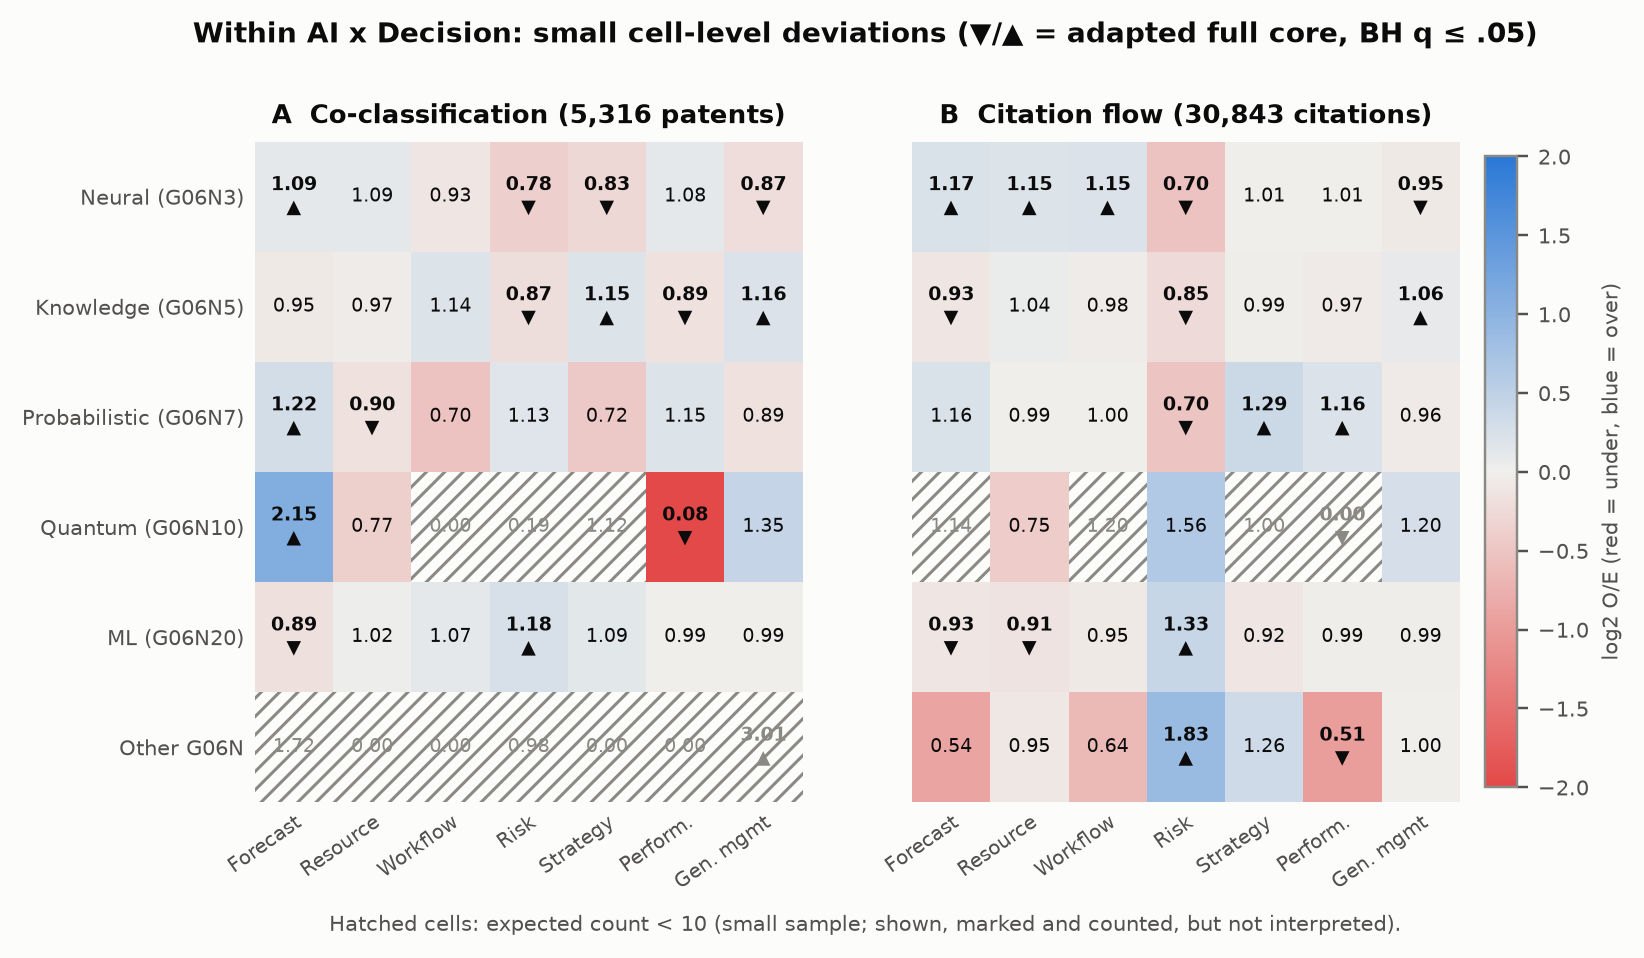
\includegraphics[width=\linewidth]{fig_cpc_heatmap.png}
  \caption{6$\times$7 CPC 矩陣中格層級的 $\log_2$ O/E：（A）共同分類，5,316 件專利；（B）申請人引用流動，30,843 筆引用。紅色表示代表不足，藍色表示過度代表。斜線格的期望次數低於 10，屬小樣本且不予詮釋，但仍予以呈現、在符合核心規則時加以標記，並納入下文的計數與表~\ref{zh:tab:cells_both}。三角形標示 M06-P 下的調整後完整核心（BH $q \le .05$；預先登錄 3，模組 P1）：A 部分為 8 個偏低／7 個偏高，B 部分為 9／8。\texttt{G06N7}~$\times$~PERFORMANCE 在 A 中沒有標記，因其僅於 B 部分屬調整後完整核心（A 部分 M06-P $q = .93$）。沒有任何偏低格在兩個時間半段中皆獲重現（第~\ref{zh:sec:study2_suite}~節）。}
  \label{zh:fig:cpc_heatmap}
\end{figure}

幅度比計數更為重要。除小樣本的量子格外，於兩部分皆偏低之五格的 O/E 介於 0.70 至 0.95 之間：這是在整體強度約為期望值三倍的領域配對內部的輕微不足。此範圍並未涵蓋 B 部分整個調整後核心：除量子格外，另有一個 B 部分核心格低於此範圍（圖~\ref{zh:fig:cpc_heatmap}）。這些格皆非分隔，本研究亦不將其稱為缺口。

\subsection{完整重現套組}
\label{zh:sec:study2_suite}

預先登錄 3 由十個模組 P1--P10 組成，每個模組為研究一的一條原始研究脈絡，在具流動效度的資料上提供一個專利類比。P1 即第~\ref{zh:sec:study2_cells}~節的檢定組。表~\ref{zh:tab:suite} 將 P2--P10 對應至其原始脈絡，表~\ref{zh:tab:app_suite} 則提供 P2、P3 與 P9 的細節。

\begin{table}[tbp]
  \centering
  \small
  \caption{完整重現套組：研究一原始脈絡的專利類比 P2--P10。DIRECT。}
  \label{zh:tab:suite}
  \setlength{\tabcolsep}{4pt}
  \begin{tabular}{l p{0.19\linewidth} p{0.24\linewidth} p{0.40\linewidth}}
    \toprule
    模組 & 原始脈絡 & 專利類比 & 結果 \\
    \midrule
    P2 & V9.1 校準 & 種子、虛無模型偽陽性率、檢定力、分段 & A：20 格恆為 $q \le .05$，4 格為邊界格；B：22 格恆為顯著，0 格為邊界格。每個虛無矩陣的平均虛假格數為 0.045（A）／0.049（B）。檢定力 67\%（A）／79\%（B） \\
    P3 & V6/V8/V9 引用脈絡 & 依時間半段進行探索／確認 & A：0 $\rightarrow$ 8 個偏低格（前半段僅 543 份文件）；B：3 $\rightarrow$ 11 個偏低格；0 個偏低格在兩個半段中皆獲重現 \\
    P4 & 研究一人工編碼稽核 & 標題關鍵詞標籤的表面效度（lift $\ge$ 1.5 即通過） & 全部 11 個標籤皆通過 \\
    P5 & V7/V11 作者 SNA & 含 Burt 限制度的公司引用網路 & AI\_FIRM$\sim$DEC\_FIRM O/E 0.24；符合預先登錄的公司層級判準（其後在專利組合虛無模型下為 \texttt{PARTIAL}）；MIXED 限制度中位數 0.36，度數匹配虛無模型為 0.444（$p = .001$） \\
    P6 & V10.1 外部審查 & 移除否證 & 10/10 名候選者被否證為不可或缺；最大聯合連通元件由 5,954 $\rightarrow$ 5,563 家公司 \\
    P7 & V10 高階網路 & 共同受讓超邊 & 2,546 條超邊；32\% 將一家 AI\_FIRM 與一家 DEC\_FIRM 或 MIXED 公司連結 \\
    P8 & V11.1 身分驗證 & 別名檢查 & 檢查 54 家公司；0 個可能的別名衝突 \\
    P9 & Gap Validity & 間接限制項；替代路徑 & 間接項為 0（對二分圖為恆等式）；每個偏低格有 20--30 條長度為 3 的替代路徑（在稠密矩陣中幾乎必然） \\
    P10 & Limitation Scout & --- & \texttt{NOT\_\allowbreak APPLICABLE}（專利沒有研究限制章節） \\
    \bottomrule
  \end{tabular}
\end{table}

\paragraph{P2：校準。} 在 20 個種子（$\times$ 10,000 次抽樣）下，B 部分的顯著集合完全相同（22 格恆為 $q \le .05$，0 個邊界格）；A 部分則有 20 格恆為顯著、4 格為邊界格。在 1,000 個端點置換虛無矩陣上（以 BH 校正的精確檢定），出現任何虛假格之矩陣的比例為 3.6\%（A）與 4.4\%（B）。這些虛無矩陣與精確檢定共享邊獨立的假設，因此無法揭露由文件內群聚所造成的反保守性。對於 $E \ge 100$ 的格，偵測 20\% 偏低的檢定力在 A 部分為 18/27 = 67\%，在 B 部分為 23/29 = 79\%，因此較弱或較小的偏低可能被遺漏。分段檢查見表~\ref{zh:tab:app_suite}。

\paragraph{P3：跨時間重現。} 偏低格數在 A 部分由 0（2010--2017）增至 8（2018--2025），在 B 部分由 3（2013--2018）增至 11（2019--2025）。無論在哪一部分，皆沒有任何偏低格在兩個半段中都獲重現。此處有兩點須注意。第一，A 部分的前半段僅有 543 份文件，檢定力不足。第二，P3 要求兩個半段皆出現顯著偏低，而研究一的時期檢查僅問方向是否維持。因此，P3 顯示的是格層級的顯著性無法跨時間重現；它並未顯示文獻型態比專利型態更為穩定。

\paragraph{P4：標籤表面效度。} 相對於其他 AI$\cup$DEC 專利，全部 11 個標籤在標題關鍵詞命中率上皆通過 1.5 的 lift 門檻；最低 lift 為 2.18（\texttt{G06N20}；所有 lift 值見表~\ref{zh:tab:app_lift}）。此檢查替代了研究一的編碼稽核，但它是標題關鍵詞檢查，而非人工稽核。

\paragraph{P5：公司網路。} 預先登錄 1 包含一項以領域層級結構洞為條件、關於受讓人（assignee）中介者的探索性 H3；由於 H1 未獲支持，H3 並未執行（修訂 A2）。P5 提出一個獨立的問題（RQ2）：無論領域層級的結果為何，公司（firm）層級是否存在結構洞；此模組在預先登錄 3 中被預先登錄為作者網路脈絡 V7 與 V11 的類比。經消歧的受讓人以申請人引用相連（排除自我引用），形成一個包含 6,201 個組織、20,681 條連結、總權重為 109,508 筆引用的網路。公司分為三組：2,926 家 AI\_FIRM（僅擁有純 AI 專利）、1,570 家 DEC\_FIRM 與 1,705 家 MIXED。群體 O/E 在 AI\_FIRM$\sim$DEC\_FIRM 為 0.24（$O = 886$，$E = 3{,}700$），在 AI\_FIRM$\sim$MIXED 為 0.81，在 DEC\_FIRM$\sim$MIXED 為 0.97。預先登錄的公司層級結構洞判準在此階段獲得滿足。Burt 限制度的中位數 \citep{burt1992structural} 在 AI\_FIRM 為 0.62，在 DEC\_FIRM 為 0.76，在 MIXED 為 0.36。相對於度數匹配的標籤置換虛無模型，MIXED 的中位數顯得偏低（虛無模型中位數 0.444；單尾 $p = .001$）。單獨來看，這正是此前提所預測的型態，但並非已確認的結構洞：標籤虛無模型固定了度數而未固定專利組合，此型態可能機械性地源自公司所擁有的專利。這一可能性促成了預先登錄 4。

\paragraph{P6：移除否證。} 度數至少為 5 且限制度最低的十家 MIXED 公司為 International Business Machines、General Electric、Tesla、ioCurrents、Google、Accenture、Amazon Technologies、T-Mobile USA、Optum Services 與 Strong Force VCN Portfolio 2019。移除全部 10 家之後，AI\_FIRM 與 DEC\_FIRM 公司仍然相連，且同時包含兩群的最大連通元件僅由 5,954 家縮減至 5,563 家：10/10 名候選者皆被否證為不可或缺的中介者。套組中的「跨群權重保留」指標在建構上恆等於 1，故本研究不據此做任何推論。

\paragraph{P7--P10。} P7（超邊）與 P8（別名）的結果見表~\ref{zh:tab:suite}。Gap Validity（P9）重複研究一的診斷：間接項為零是恆等式，而每個偏低格有 20--30 條長度為 3 的替代路徑，在稠密的 6$\times$7 矩陣中幾乎必然成立；兩者皆非證據。Limitation Scout（P10）是對論文所陳述之研究限制的檢查，不適用於專利。

\subsection{保留專利組合的公司虛無模型}
\label{zh:sec:study2_firm}

P5 的型態可能是機械性的。MIXED 公司同時擁有兩類專利，而專利主要引用其自身領域，因此即使沒有任何公司從事中介，位於不同領域的專門型公司（specialist firm）彼此之間的引用仍會很少。預先登錄 4 是在 P5 結果已知之後撰寫，並受其促成；其統計量、分層與決策規則則在計算任何一次重複之前即已凍結。其虛無模型，即保留專利組合的虛無模型（portfolio-preserving null），在分層內置換專利的擁有者集合，固定每家公司的專利組合與群體，以及整個專利層級的引用網路。主要分層為專利類型 $\times$ 核准年份（48 層）；技術組合分層（S-tech）為類型 $\times$ 年份 $\times$ AI 列 $\times$ DEC 欄（1,795 層）。每個虛無模型有 1,000 次重複，方案 $s$ 的第 $r$ 次重複使用種子序列 [20261119, $s$, $r$]。

\paragraph{範圍。} 此虛無模型以全部 127,114 件範圍內專利、擁有其中任一件的 14,600 家公司，以及其間的 162,339 筆申請人引用為起點。P5 僅報告移除自我引用後至少有一條公司間連結的 6,201 家公司（20,681 條連結；總權重 109,508）。恆等置換（每個擁有者集合皆保持原位）可精確重現 P5 的數值，因此兩組數字描述的是同一網路在兩個篩選階段的狀態。

\paragraph{虛無模型未固定之處。} 此虛無模型保留每家公司依類型與年份計算的專利組合件數，但未保留其度數或連結強度。限制度高度依賴度數 \citep{everett2020unpacking}，因此 T2 無法區分中介與度數。P5 的度數匹配標籤虛無模型（虛無模型中位數 0.444）與專利組合虛無模型（虛無模型中位數 0.104）回答的是不同的問題，且兩者皆未同時固定度數與專利組合。

\begin{table}[tbp]
  \centering
  \small
  \caption{保留專利組合的公司虛無模型：每種分層 1,000 次重複，附單尾（下尾）$p$ 值。T1 為專門型 AI 公司與決策公司之間連結的 O/E，T2 為 MIXED 公司的 Burt 限制度中位數。T1 符合其判準而 T2 不符合，因此兩種分層下的判定皆為 \texttt{PARTIAL}。此虛無模型並未保留公司度數。DIRECT。}
  \label{zh:tab:firm_null}
  \footnotesize
  \setlength{\tabcolsep}{4pt}
  \begin{tabular}{p{0.22\linewidth}rlrlr}
    \toprule
    & & \multicolumn{2}{c}{主要（類型 $\times$ 年份）} & \multicolumn{2}{c}{S-tech（+ 技術組合）} \\
    統計量 & 觀察值 & 虛無模型中位數 [95\%] & $p$ & 虛無模型中位數 [95\%] & $p$ \\
    \midrule
    T1 OE(AI\_FIRM$\sim$\allowbreak DEC\_FIRM) & 0.240 & 0.356 [0.317--0.398] & .001 & 0.307 [0.277--0.345] & .001 \\
    T2 MIXED 限制度中位數 & 0.358 & 0.104 [0.098--0.111] & 1.000 & 0.116 [0.110--0.122] & 1.000 \\
    OE AI\_FIRM$\sim$\allowbreak MIXED & 0.809 & 1.000 & .001 & 0.985 & .001 \\
    OE DEC\_FIRM$\sim$\allowbreak MIXED & 0.970 & 1.009 & .001 & 1.025 & .001 \\
    \bottomrule
  \end{tabular}
\end{table}

\paragraph{結果。} 結果見表~\ref{zh:tab:firm_null} 與圖~\ref{zh:fig:firm_null}。在兩種分層下，觀察到的專門型 O/E（T1 = 0.240）皆低於每一次虛無重複（$p = .001$，即 1,000 次重複所能達到的最小值）。然而，虛無模型中位數（0.356 與 0.307）本身即遠低於 1，且殘差的大小取決於所採用的尺度。在「與 1 之差距」的尺度上，固定專利組合的虛無模型重現了 T1 低於 $O = E$ 之觀察不足的 85\%（主要）與 91\%（S-tech），剩下 15\% 與 9\%。在比值尺度上，觀察到的專門型連結為虛無期望值的 0.240/0.356 = 0.67 與 0.240/0.307 = 0.78，即不足 33\% 與 22\%。兩種解讀皆屬有效，且回答的是不同的問題：專利組合能解釋與均等之間多少距離，以及真實連結比專利組合所隱含者低多少。專門型 AI 公司與決策公司之間的連結顯著少於其專利組合所隱含的水準；這並不表示有任何一方在兩者之間從事中介，本研究亦不將其稱為結構洞。

T2 未符合其判準。觀察到的 MIXED 限制度中位數（0.358）高於每一次虛無重複（虛無模型中位數 0.104 與 0.116；$p = 1.000$）：真實公司的群聚程度高於專利組合虛無模型所隱含者。由於此虛無模型未保留度數，此比較無法分離出中介。兩種分層下的判定皆為 \texttt{PARTIAL}，因此判定並不取決於技術組合。\texttt{PARTIAL} 表示「超越專利組合之組織結構洞」的雙判準規則並未滿足（表~\ref{zh:tab:app_prereg}）：公司層級的結構洞未獲確認。這並不表示結構洞已被排除，且 T1 已獲滿足。

\begin{figure}[tbp]
  \centering
  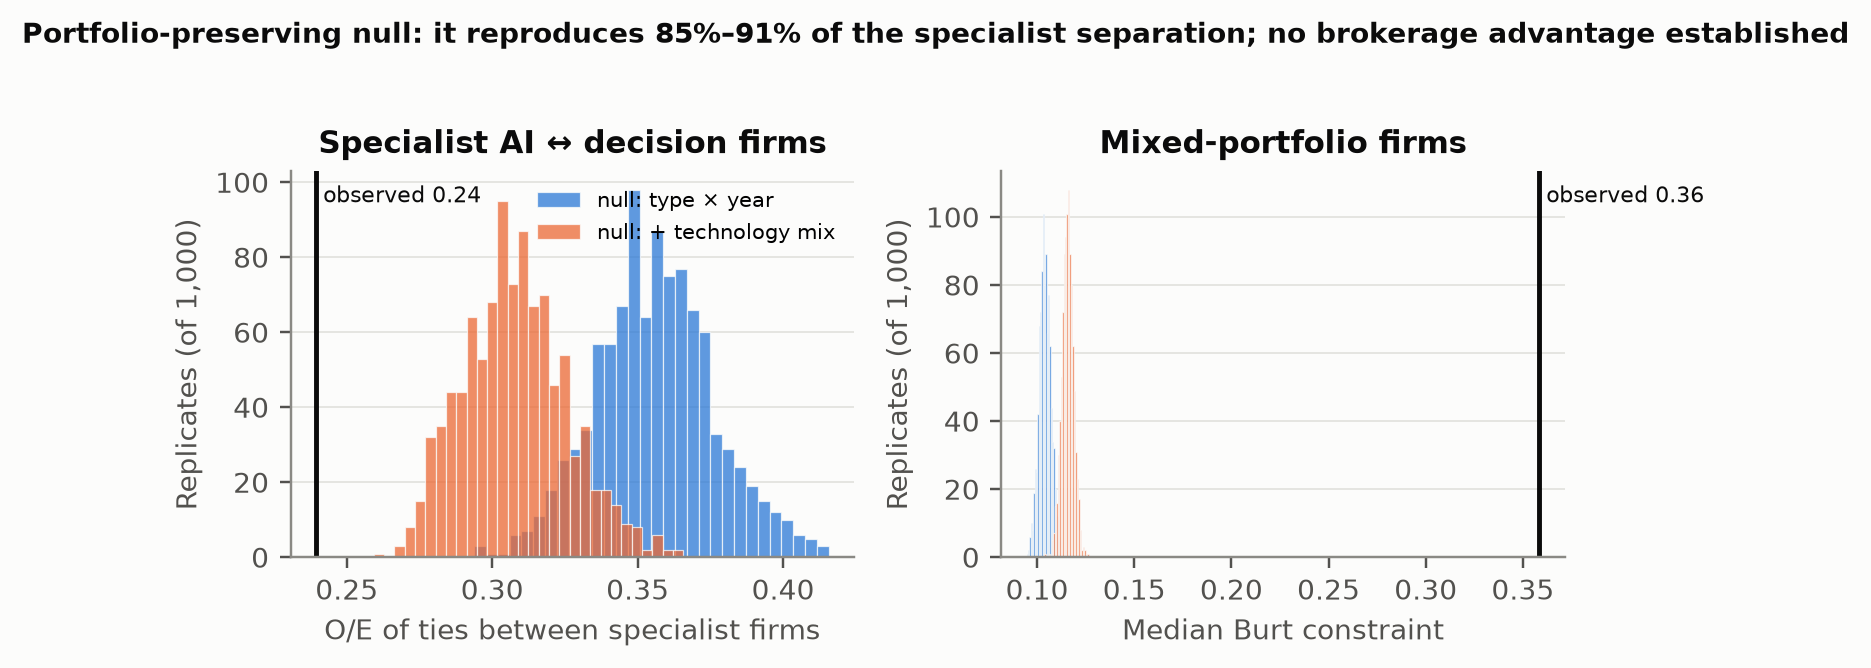
\includegraphics[width=\linewidth]{fig_firm_null.png}
  \caption{保留專利組合的公司虛無模型：在主要（類型 $\times$ 年份；藍色）與 S-tech（+ 技術組合；橙色）分層下各 1,000 次重複。專利組合、群體與專利層級的引用網路皆予固定；公司度數則未固定。左圖：T1，專門型 O/E（各 $p = .001$）；虛無模型重現了與 1 之差距的 85\% 與 91\%，而觀察到的連結為虛無模型中位數的 0.67 與 0.78（不足 33\% 與 22\%）。右圖：T2，MIXED 限制度中位數（各 $p = 1.000$）；此圖無法區分中介與度數，因此並未確立中介優勢。判定：兩種分層下皆為 \texttt{PARTIAL}；公司層級的中介仍未解決。}
  \label{zh:fig:firm_null}
\end{figure}

與 P5 的對比——相對於度數匹配的虛無模型，MIXED 的限制度偏低；相對於保留專利組合的虛無模型，則偏高——顯示虛無模型的選擇決定了對中介的解讀（第~\ref{zh:sec:discussion_measurement}~節）；由於專利組合虛無模型是受 P5 結果所促成，此一反轉屬於受資料啟發的後續分析。因此，RQ2 仍未解決。超越專利組合的專門型分隔是顯著的（兩種分層下皆為 $p = .001$），而 P5 的度數匹配虛無模型亦傾向 MIXED 公司具有較低的限制度（$p = .001$）；然而，沒有任何可用的虛無模型能同時固定度數與專利組合，因此混合型公司是否在此分隔中從事中介，無法在此判定。

% ============================================================
% ch5_discussion.tex -- 第五章：討論、多層規劃議程與研究限制
% 譯自 paper/en/back.tex 第 6--8 節（Integrative Discussion, MLP Agenda, Limitations）。
% 所有數字取自 raw_materials/experimental_log.md；多層規劃模型常數為
% raw_materials/idea.md 之 v1.0 正式規格。治理型態 C／F／D 不得展開為任何名稱。
% ============================================================

\chapter{討論、多層規劃議程與研究限制}
\label{zh:ch:discussion}

\section{綜合討論}
\label{zh:sec:discussion}

\subsection{三條資料線共同顯示的結果}
\label{zh:sec:discussion_lines}

在三條資料線中，唯有專利資料提供了具外部指派群體標籤之行動者之間的有向二元流動，而這正是中介（brokerage）分析所需要的資料 \citep{gould1989structures}；研究一的引用資料線原則上可能承載此類流動，但因資料與設計上的原因而未能達成（第~\ref{zh:sec:study1_network}~節），且沒有任何公開資料來源通過流動效度關卡（表~\ref{zh:tab:app_sources}）。三項專利分析共用同一資料來源，並非彼此獨立的複製研究。

綜合來看，這些資料線支持以下四項陳述。第一，在領域層次上，依本研究之定義，AI 與決策技術呈現過度連結（over-connection），而非彼此分隔，且此結果在各種設定下皆穩健；此過度連結正在下降，儘管其預先登錄（preregistration）標籤為 \texttt{PERSISTENT}（第~\ref{zh:sec:study2_aggregate}~節；圖~\ref{zh:fig:patent_trend}），且在排除 G06Q10/04 以及採用粒度匹配的參照集時，判定仍然成立（表~\ref{zh:tab:construct}；第~\ref{zh:sec:lim_measurement}~節）。第二，在此一過度連結的領域配對之內，格層次的偏低大多幅度有限，且無法在前後兩半時期中複製（第~\ref{zh:sec:study2_suite}~節；圖~\ref{zh:fig:cpc_heatmap}）。第三，在公司層次上，超出專利組合構成所能解釋的部分之外，仍存在顯著的專門型公司（specialist firm）分隔（分別佔與 1 之差距的 15\% 與 9\%；以比值尺度衡量則短缺 33\% 與 22\%），而混合型（多角化）公司（mixed-portfolio firm）是否對此分隔進行中介，則仍未解決（第~\ref{zh:sec:study2_firm}~節；圖~\ref{zh:fig:firm_null}）。第四，沒有任何資料線證實 Burt 意義上的結構洞（structural hole）：研究一的網路資料線找到 0 個經證實的中介者（HISTORICAL / USER\_REPORTED），而 CORDIS 二分網路（bipartite network）虛無模型（null model）則找到 0 個顯著候選者。

這些結果看似與研究一相互矛盾：在研究一中，全部 16 個偏低的功能配對在兩個時期皆維持偏低。然而兩者涉及不同的分析單位與參照基準。研究一探討的是哪些「功能配對」在文件中共現（co-occurrence），其參照為一個封閉之 $10\times12$ 矩陣的邊際；由於期望次數的總和等於觀察總數，部分格的偏低必然意味著其他格的偏高（核心格中兩者各有 16 個）。偏低格（depleted cell）描述的是既有連結的「組成」，而非其「數量」。研究二探討的則是兩個「技術領域」彼此交換引用的強度，其參照為 179 個可比較的領域。兩者的持續性判準亦不相同——研究一僅看方向，專利研究則要求三項檢定在前後兩半時期皆顯著（其中一半樣本較小）——因此兩者的對比並非同類比較。在兩條資料線中，格層次的發現皆為一個相互連結之整體內部的相對偏離，而非分隔的證據。綜合而言，證據並不支持 AI 與決策技術之間的知識流動（knowledge flow）存在結構洞（RQ1）。在公司層次（RQ2），結構洞既未獲證實，亦未被排除：判定結果為 \texttt{PARTIAL}，且目前沒有任何可用的虛無模型能同時固定度數與專利組合。本研究不主張任何因果效果。

\subsection{對缺口研究的測量啟示}
\label{zh:sec:discussion_measurement}

本研究計畫記錄了共現資料與隸屬（affiliation）資料的四種失效模式，每一種皆有直接證據。\textbf{投影派系（projection cliques）：}CORDIS 共同成員關係的投影會人為製造封閉性（第~\ref{zh:sec:theory_cooccurrence}~節），而在投影之後計算的中介並非二模中介 \citep{jasny2015two}。\textbf{限制度在二分網路中的退化：}在嚴格的二分網路中，網路限制度（network constraint）會退化為二元集中度——而批評者早已指出，這正是主導該指標的成分 \citep{everett2020unpacking,johnson2026reassessing}。這是一個恆等關係；而在 120 格中有 104 格具觀察值的矩陣中，或在一個稠密的 $6\times7$ 矩陣中，每一個偏低格周圍都能找到替代路徑幾乎是必然的；這些缺口效度（Gap Validity）檢查是對資料結構的診斷，而非關於這些領域的證據。\textbf{同詞兩端共用}（same-term self-pairing）與\textbf{模型推論標籤}（model-inferred labels）（第~\ref{zh:sec:study1_direction}~節與第~\ref{zh:sec:study1_reliability}~節）屬於非隨機誤差。隨機、非差異性的誤分類（misclassification, non-differential）只會削弱偏低，但在邊際固定的矩陣中，膨脹某一格會機械性地使其所在列與欄的其餘部分偏低。在研究一中，此機制並非主要驅動因素：排除同詞紀錄後，13/16 個偏低格維持其方向，而移除同詞兩端共用的紀錄僅使核心格減少 2 格。模型推論標籤仍是一個未經檢驗的非隨機誤差來源，因此該方向僅屬描述性，且未獲證實。結構洞測度在不同資料類型之間無法互換 \citep{saglietto2020research}；這四種機制具體說明了其原因。前兩者為已知結果；本研究計畫補充的是它們對缺口推論的影響。

有兩項啟示涉及虛無模型。第一，當每份文件皆貢獻一個完整的列 $\times$ 欄區塊時，保留文件結構的交換虛無模型（M06）會退化；M06-P（專利適用之保留文件結構虛無模型）雖保留了該結構，但未經型一錯誤校準（第~\ref{zh:sec:study2_cells}~節）。第二，公司限制度的解讀取決於虛無模型固定了什麼：相對於度數配對的標籤置換虛無模型，混合型公司看似具有較低的限制度（$p=.001$）；相對於保留專利組合的虛無模型（portfolio-preserving null），其限制度則高於預期（$p=1.000$）。前一個虛無模型忽略了公司擁有什麼，後一個則忽略了公司有多少連結；用於檢驗中介的虛無模型必須同時固定兩者。

由此可得三項設計上的啟示。檢定應採相對比較，因為跨領域的 O/E 低於 1 乃是常態。決策規則應在檢視真實資料之前先以合成資料加以校準，且所用的生成器應比本研究所用者更不簡化。規則、停止規則（stop rule）與修訂（amendment）應事先固定並據實報告（表~\ref{zh:tab:app_prereg} 與表~\ref{zh:tab:app_amend}），且最好透過第三方登錄平台為之。對缺口研究而言，實務意涵很簡單：偏低格並不等於缺口；低限制度的節點也不是中介者，除非它能通過一個同時保留專利組合與度數的虛無模型的檢驗。

\subsection{負面結果尚未釐清之處}
\label{zh:sec:discussion_hypothesis}

本研究所檢驗的前提，是本研究計畫自身由共現證據所導出的工作前提。未能找到知識流動上的結構洞，並不證明結構洞不存在，但它移除了將 AI 與決策之整合視為一個「橋接問題」的一項理由。它既未確立困難所在，也未使任何單一替代解釋變得更為可能：研究一與研究二不含任何組織內部資料，而專利公司網路所記錄的是受讓人（assignee）之間的引用，而非公司如何部署 AI。至少有五項候選解釋仍屬未決，而本研究的資料對其中任何一項皆無直接的證據力。(1)~\textbf{組織資源分配（resource allocation）與決策權（decision rights）：}預算、核准鏈與治理規則允許或禁止 AI 的特定用途，並規範人類與 AI 在決策中如何配置。(2)~\textbf{資料品質：}流程所需的資料缺漏、品質不佳或未經整合。(3)~\textbf{成本：}整合可行且獲得允許，但其預期價值不足以支應其成本。(4)~\textbf{法規與責任：}外部規則或責任歸屬要求由人類做出決策，或禁止自動化。(5)~\textbf{任務適配性：}AI 在該任務上表現不佳，或該任務具有不確定性或多義性，而有利於人類判斷 \citep{jarrahi2018artificial}；不同的決策任務條件有利於不同的人機結構 \citep{shrestha2019organizational}。這些解釋並非互斥，且其中數項可能同時在同一家公司中產生約束。

組織層面的候選解釋，正是本研究計畫之模型所表徵的那一項。它借鑑了「經濟行動鑲嵌於具體、持續之關係中」的觀點 \citep{granovetter1985economic}，以及第~\ref{zh:sec:intro}~章所回顧的管理文獻 \citep{shrestha2019organizational,raisch2021artificial,berente2021managing}；這些文獻為模型的層級設計提供了動機，但既未檢驗該模型，也未使其優於其他候選解釋。究竟是哪一項候選解釋在組織內部或外部產生約束，正是研究三設計來加以區辨的問題（第~\ref{zh:sec:mlp_study3}~節）。

% ------------------------------------------------------------
\section{多層規劃研究議程}
\label{zh:sec:mlp}

本節是負面結果的後續延伸，而非由該結果推得的結論。它僅將第~\ref{zh:sec:discussion_hypothesis}~節中的組織候選解釋加以形式化；該解釋涉及不同行動者之間的巢狀決策：企業分配資源，架構與治理層決定 AI 整合與受監督的深度，而流程負責人則選擇人機配置，且每一方皆預期其下層行動者的回應。這正是多層規劃（multi-level programming, MLP）的結構：領導者（leader）在追隨者（follower）之最適回應的限制下進行最佳化 \citep{dempe2002foundations,colson2007overview}。

\subsection{形式模型}
\label{zh:sec:mlp_model}

令 $i\in I$ 為決策流程的索引，$r\in\{D,A,R,G\}$ 為能力資源（資料、AI、可靠性與治理）的索引，每項資源皆以順序尺度 $\{0,1,2,3\}$ 衡量；$\kappa_i$ 為流程的後果等級（與 Cohen's $\kappa$ 無關）。企業的預算為 $B_{\mathrm{tot}}$，並在治理型態（governance regime）$\Gamma\in\{C,F,D\}$ 下運作；在原型中，治理型態僅是一組參數：容量 $K_\Gamma$、風險、成本與彈性的乘數，以及許可矩陣 $\mathrm{Allow}_{m\Gamma}$（表~\ref{zh:tab:app_regimes}）。正式的 v1.0 模型共有三層，其完整陳述見附錄~\ref{zh:app:mlp_full}：
\begin{itemize}
\item \textbf{第一層（領導者）}在預算內分配整數資源 $b_i^r$，以提高能力上限 $\bar D_i,\bar A_i,\bar R_i,\bar G_i$，並最大化 $F_1$；$F_1$ 為已實現價值與 AI 採用數的加權和，減去資源使用量與剩餘風險，各項皆於追隨者的回應下評估。
\item \textbf{第二層}為每個流程選擇 AI 整合深度 $A_i$、人類監督 $H_i$、工作流程整合 $WI_i$ 與保證 $EA_i$，以最大化 $F_2$；其限制條件包括能力上限、隨 $A_i$ 與 $\kappa_i$ 提高的要求門檻（表~\ref{zh:tab:app_thresholds}），以及由所有流程共用的治理容量 $K_\Gamma$。附錄~\ref{zh:app:mlp} 列出 $F_2$ 及其組成項，以及其未經校準的設計權重（式~\eqref{zh:eq:app_f2}）。
\item \textbf{第三層（追隨者）：}每個流程選擇一種獲許可的配置——\texttt{HumanOnly}、\texttt{AIAssist}、\texttt{HumanFirstAICheck}、\texttt{AIFirstReview} 或 \texttt{BoundedAutomation}——其最低第二層要求從 \texttt{HumanOnly} 的「無要求」逐步提高至 \texttt{BoundedAutomation} 的最高要求（表~\ref{zh:tab:app_configs}）。
\end{itemize}
在選擇型流程中，固定的分數門檻 $\tau_i$ 決定 AI 的建議（式~\eqref{zh:eq:mlp_tau}）；它是一種敏感度分析工具，而非錯誤率的模型。

\paragraph{性質、範圍與錨定。}在五項假設下，所選定的三層解組合存在，且窮舉式逆向歸納必然終止（附錄~\ref{zh:app:mlp}）；對此一有界原型進行精確窮舉，並不構成可處理性（tractability）的主張 \citep{jeroslow1985polynomial}。v1.0 原先作為門檻錨定的研究一 16 個 V9 偏低格已予撤回：它們並非經驗上已驗證的缺口，且其方向未獲證實（第~\ref{zh:sec:discussion_measurement}~節）。每一項門檻、權重與許可皆為設計假設，唯有在組織候選解釋通過研究三的檢驗時，才會在研究三中加以校準。

\subsection{模擬示例}
\label{zh:sec:mlp_sim}

所有係數皆為模擬值，輸出結果不描述任何真實公司。表~\ref{zh:tab:back_mlp_scenarios} 與圖~\ref{zh:fig:mlp_scenarios} 報告九個基準情境（三個流程；治理型態 C、F 與 D；預算 3、5 與 7；所有配置皆獲許可），以精確逆向歸納求解；針對 768 個案例所進行的一致性檢查發現，與正式限制式之間的不一致為 0 件（附錄~\ref{zh:app:mlp}）。

\begin{table}[tbp]
\centering
\caption{三層原型之模擬基準情境（SIMULATED；無公司資料）。治理型態僅為參數集合（表~\ref{zh:tab:app_regimes}）。}
\label{zh:tab:back_mlp_scenarios}
\small
\setlength{\tabcolsep}{4pt}
\begin{tabular}{lrrrrrl}
\toprule
治理型態 & 預算 & $F_1$ & \begin{tabular}[b]{@{}r@{}}實現\\價值\end{tabular} & \begin{tabular}[b]{@{}r@{}}剩餘\\風險\end{tabular} & \begin{tabular}[b]{@{}r@{}}AI\\採用數\end{tabular} & 配置（三個流程） \\
\midrule
C & 3 & 1.708 & 1.560 & 0.268 & 2 & \texttt{AIAssist} $\times2$，\texttt{HumanOnly} $\times1$ \\
F & 3 & 1.775 & 1.642 & 0.316 & 2 & \texttt{AIAssist} $\times2$，\texttt{HumanOnly} $\times1$ \\
D & 3 & 1.842 & 1.724 & 0.363 & 2 & \texttt{AIAssist} $\times2$，\texttt{HumanOnly} $\times1$ \\
\midrule
C & 5 & 2.158 & 2.221 & 0.451 & 3 & \texttt{AIAssist} $\times3$ \\
F & 5 & 2.244 & 2.338 & 0.530 & 3 & \texttt{AIAssist} $\times3$ \\
D & 5 & 2.331 & 2.454 & 0.610 & 3 & \texttt{AIAssist} $\times3$ \\
\midrule
C & 7 & 2.158 & 2.221 & 0.451 & 3 & \texttt{AIAssist} $\times3$（與預算 5 相同） \\
F & 7 & 2.244 & 2.338 & 0.530 & 3 & \texttt{AIAssist} $\times3$（與預算 5 相同） \\
D & 7 & 2.616 & 3.286 & 0.736 & 3 & \texttt{AIAssist} $\times2$，\texttt{HumanFirstAICheck} $\times1$ \\
\bottomrule
\end{tabular}
\end{table}

\begin{figure}[tbp]
\centering
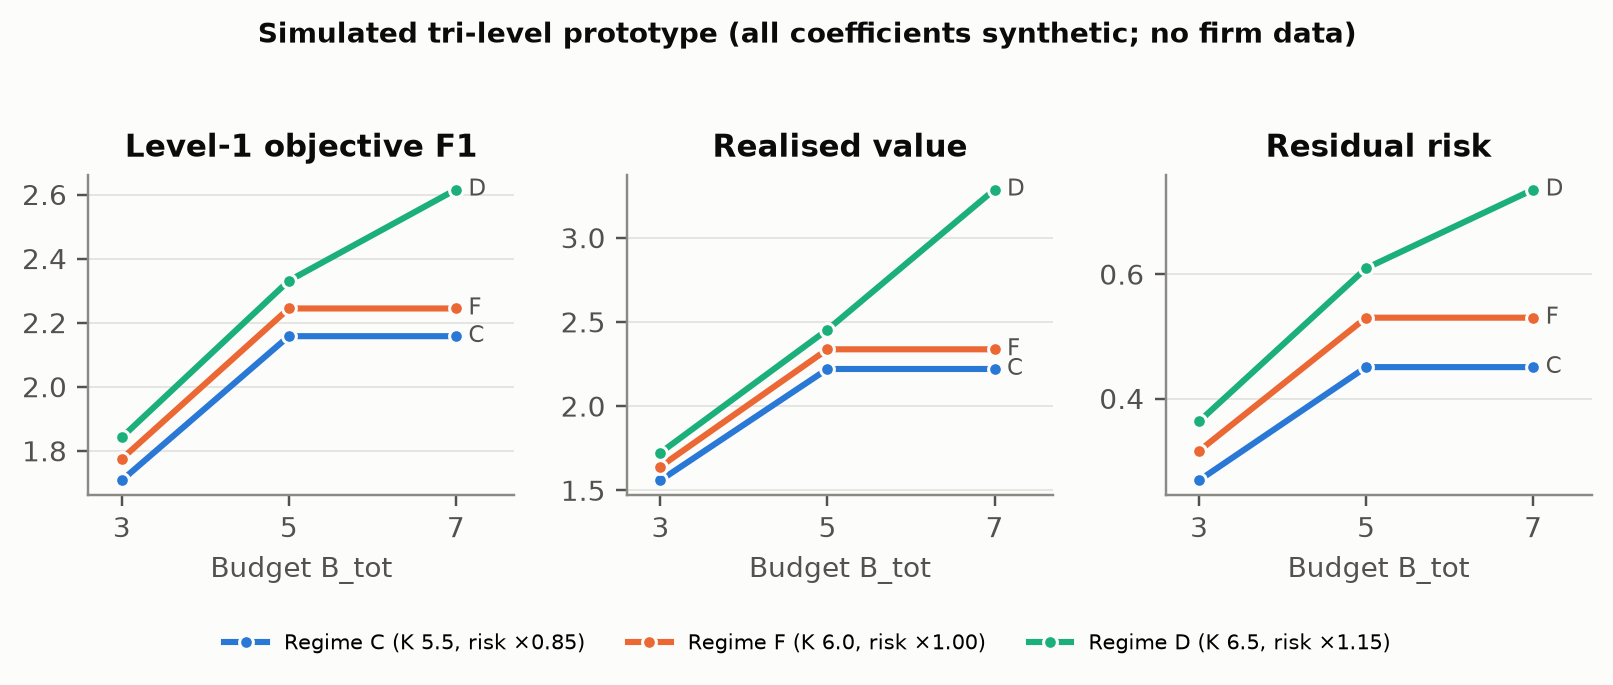
\includegraphics[width=\linewidth]{fig_mlp_scenarios.png}
\caption{模擬之三層原型：在預算 $B_{\mathrm{tot}}\in\{3,5,7\}$ 下，治理型態 C（$K$ 5.5，風險 $\times0.85$）、F（$K$ 6.0，風險 $\times1.00$）與 D（$K$ 6.5，風險 $\times1.15$）的第一層目標 $F_1$、實現價值與剩餘風險。所有係數皆為模擬值；未使用任何公司資料，輸出結果亦不描述任何真實公司。在 C 與 F 之下，預算 7 的解與預算 5 的解相同；在 D 之下，預算 7 時有一個流程改採 \texttt{HumanFirstAICheck}。}
\label{zh:fig:mlp_scenarios}
\end{figure}

此模式是機械性的：在每一預算水準內，$F_1$、實現價值與剩餘風險皆依 C、F、D 的順序遞增，這反映的是治理型態的參數設定，而非組織的任何特性。

兩項探測僅用以說明模型機制，而非研究發現。在「治理許可探測」（治理型態 C，預算 5）中，\texttt{AIAssist} 被禁止：$F_1$ 從 2.158 降至 0.837，配置則從 \texttt{AIAssist} $\times3$ 變為 \texttt{HumanOnly} $\times2$ 加上 \texttt{HumanFirstAICheck} $\times1$。治理型態與預算皆未改變，但第一層會重新最佳化其分配，因此能力是內生的，而非保持固定。此一轉變在建構上即由許可所驅動，因為移除最適配置會迫使模型改採次一順位的可行配置；研究三必須在資料中觀察到此類模式。在「選擇門檻探測」（治理型態 F，預算 5）中，流程 P2 的分數為 0.65，真實結果為 1。當 $\tau\leq0.6$ 時，P2 採用 \texttt{AIAssist}（$F_1$ 2.244，即 F/5 基準）；當 $\tau=0.7$ 時，AI 的建議錯誤，第一層不再分配任何資源給 P2 的 AI 能力，P2 因而退回 \texttt{HumanOnly}（$F_1$ 1.450）。由於分數與結果固定且為各層所知，此探測對錯誤率不具任何意涵。

\subsection{研究三：預先登錄之企業研究（計畫，而非結果）}
\label{zh:sec:mlp_study3}

研究三依序有兩個目標：其一是在第~\ref{zh:sec:discussion_hypothesis}~節的五項候選解釋之間加以區辨；其二是唯有在組織候選解釋獲得支持時，才對模型進行校準。目前尚未蒐集任何資料。

\paragraph{競爭解釋（competing explanations）及其特徵。}各候選解釋的差異在於：將 AI 整合進某一決策流程的嘗試會在「何處」停止，以及必須改變「什麼」才能使其繼續推進（表~\ref{zh:tab:back_study3_rivals}）。所有特徵皆為觀察性的。當可行且獲許可的配置因其整合成本即使在重新分配後仍超出預算而遭拒絕時，即為成本構成約束；當總體上存在預算、但領導者將其分配至他處，或內部決策權阻擋採用時，則為分配構成約束。內部決策權與外部法規的差別，在於構成約束的規則源自公司內部或外部。

\begin{table}[tbp]
\centering
\caption{研究三（計畫）：候選解釋、其在模型中的對應項，以及各自在整合事件中所預測的觀察特徵。目前尚未蒐集任何資料。}
\label{zh:tab:back_study3_rivals}
\footnotesize
\begin{tabular}{p{3.0cm}p{3.2cm}p{8.0cm}}
\toprule
候選解釋 & 模型對應項 & 預測特徵 \tabularnewline
\midrule
\raggedright 組織分配與決策權 & \raggedright $b_i^r$、$\mathrm{Allow}_{m\Gamma}$（內部）、$K_\Gamma$ & \raggedright 總體上存在預算，但領導者已將其分配作其他用途；或某項內部核准、決策權或治理容量阻擋了一個符合能力與資料要求的事件；在內部重新分配或規則改變後，該事件得以繼續推進，而其商業論證、能力或資料皆未改變 \tabularnewline
\raggedright 資料品質 & \raggedright $\bar D_i<D_{\mathrm{req}}$、$\bar R_i<R_{\mathrm{req}}$ & \raggedright 事件停止於資料就緒度或可靠性檢查；在資料補正後即可繼續推進，而規則未有改變 \tabularnewline
\raggedright 成本 & \raggedright $c_i^r$ 相對於 $B_{\mathrm{tot}}$ & \raggedright 可行且獲許可的配置因其整合成本即使在重新分配後仍超出預算而遭拒絕；拒絕理由援引的是絕對成本或報酬，且內部重新分配或規則改變無法使其翻轉 \tabularnewline
\raggedright 法規與責任 & \raggedright $\mathrm{Allow}_{m\Gamma}$（外部） & \raggedright 事件停止於援引外部規則或責任歸屬的法務或法遵審查；內部規則改變時，此阻擋並不改變 \tabularnewline
\raggedright 任務適配性 & \raggedright $\bar A_i$、$s_i$、$\tau_i$ & \raggedright 事件在針對 AI 於該任務之表現進行試行或評估後停止；流程負責人援引的是準確度或決策的多義性 \tabularnewline
\bottomrule
\end{tabular}
\end{table}

\paragraph{分析單位、抽樣與編碼。}分析單位為決策流程，即具有可辨識負責人的經常性管理決策；觀察事件為「整合事件」（integration episodes），即有文件記錄的 AI 配置提案、試行或部署及其結果（採用、修改或停止）。研究場域為一家匿名化的製造業公司，亦可能不只一家；抽樣框架、觀察期間與最低資訊樣本數將在研究三自身的預先登錄中確定。「基於能力條件可行、但因許可而受阻」必須是觀察所得，而非由模型推論而來。每一停止點「之前」所記載的紀錄（核准、預算分配、商業論證、決策權矩陣、能力或資料評估），並以訪談加以補充（但不以訪談取代），用以辨識每一事件於何處、因何原因停止。由兩位獨立的人類編碼者對每一事件的首個約束條件（first binding constraint；五項候選解釋之一，或「無法判定」）進行編碼，並在任何結果分析之前報告兩者的一致性；鑑於研究一的經驗，模型輔助編碼將不會用以取代人類編碼。

\paragraph{決策規則與停止規則。}規則與門檻將在取得資料之前凍結 \citep{nosek2018preregistration}；附錄~\ref{zh:app:study3} 完整陳述這些規則，並列出規劃中的資料（表~\ref{zh:tab:back_study3}）以及一項以真實組織關係進行的選擇性網路檢定。簡言之，若某一候選解釋是最常出現的首個約束條件，且超過預先登錄的比例，則該解釋獲得支持；否則結果即為混合，且不對模型進行校準。若具可判定約束條件的事件過少，研究即因不具資訊性而停止。研究三為觀察性研究：它能辨識哪一項限制最先產生約束，但無法辨識移除該限制的因果效果。

% ------------------------------------------------------------
\section{研究限制}
\label{zh:sec:limitations}

\subsection{構念效度與測量}
\label{zh:sec:lim_measurement}

\paragraph{研究一。}編碼的信度偏低。人類編碼者之間的一致性（AI 家族 $\kappa$ 0.05，決策家族 0.14）僅建立在 $n=20$ 筆紀錄上，本身即不精確；而兩個模型之間的一致性顯示的是可重現性，而非人類的評分者間信度（inter-rater reliability）。在符合現實的誤分類程度下，偏低格會失去顯著性，因此它們並非「16 個統計上穩健的偏低配對」。解析式的削弱界限僅涵蓋非差異性誤差，隨機誤差模型與觀察到的幅度並不吻合（第~\ref{zh:sec:study1_reliability}~節），而同詞兩端共用與模型推論標籤屬於非隨機誤差，可能在邊際固定的矩陣中造成偏低。移除分析的證據顯示，同詞兩端共用並非主要驅動因素（排除同詞紀錄後，13/16 個格維持其方向），但模型推論標籤的影響尚未經檢驗；因此該方向未獲證實。編碼者之間對於何者構成決策功能，在實質認定上亦有分歧。偏低核心格通過嚴格篩選的比例高於其他格（38\% 對 28\%）；本研究不據此作進一步推論。V6--V11.1 的網路結果屬於 HISTORICAL / USER\_REPORTED，且未經重新驗證。

\paragraph{研究二。}CPC 分類是知識領域的代理指標，而 CPC 分類之間的引用衡量的是技術鄰近性，而非 AI 融入管理決策的程度。G06Q10/04（預測與最佳化）在方法上與 AI 重疊，且與 AI 的連結較為緊密（OE 3.83），但僅佔 DEC 的一小部分（37,501 件專利中的 5,893 件）。計畫 5 受資料啟發的構念效度（construct validity）檢查顯示，領域層次的判定在所檢驗的兩種類別定義（/04 + /06；僅 /06）與兩種參照粒度下皆成立；在粒度匹配的參照集下，H1a 百分位數降至約 84--90\%（表~\ref{zh:tab:construct}）。此判定仍是關於這些 CPC 構念的陳述，而非關於整體決策的陳述。標籤效度依據的是標題關鍵詞提升度（lift）檢查（表~\ref{zh:tab:app_lift}），而非人工稽核。審查員引用（examiner citation）僅透過 PatentsView 的引用類別予以排除 \citep{alcacer2006patent,uspto2026patentsview}，因此僅含申請人引用（applicant citation）的設定實際上自 2013 年起算。資料僅涵蓋美國專利，公司身分仰賴經消歧的受讓人資料，別名檢查涵蓋 54 家公司，且沒有任何外部組織資料來源通過流動效度關卡。

\subsection{統計推論與校準}
\label{zh:sec:lim_inference}

所有結果皆為相關性結果；本研究不主張任何因果效果。未能支持結構洞的存在，並不證明在其他資料、其他操作化方式或其他國家中不存在結構洞。有四項校準上的不足限定了這些檢定的解讀。
(a)~\textbf{群聚（clustering）。}邊層次的精確檢定與原始紀錄檢定將各條邊視為獨立，然而每份文件會貢獻數條邊（研究一：1,729 份已解析文件產生 2,180 條邊；B 部分：30,843 筆引用產生 66,056 條邊）。P2 的偽陽性校準所使用的端點置換（stub-permutation）虛無矩陣同樣採用此一假設，因此無法偵測文件內群聚所造成的反保守性（anti-conservatism）。
(b)~\textbf{M06-P。}此專利適用的虛無模型未經單獨的型一錯誤校準，其虛無假設僅透過其所保留的內容（兩組邊際與區塊結構）加以陳述。
(c)~\textbf{「核心格」。}核心格（core）結合了各檢定內的 Benjamini--Hochberg 控制 \citep{benjamini1995controlling} 與相依檢定之間的一致性。因此它沒有單一明確定義的偽發現率，應被解讀為一種保守的篩選。
(d)~\textbf{合成資料校準。}生成器相當簡單（領域內引用並植入抑制）。其無結構洞基準（OE 0.388）接近參照最低四分位數（0.356），而真實的 OE（3.05）則遠高於 AI 側的最低四分位數（0.787），因此此校準對於真實基準下的檢定力所能說明者有限。
此外，在 $E\geq100$ 的格中偵測 20\% 偏低的格層次檢定力為 67\%（A 部分）與 79\%（B 部分），因此較弱的偏低或較小的格可能被遺漏，且領域層次的彙總可能掩蓋異質性。

在公司層次上，保留專利組合的虛無模型並未保留度數或連結強度，因此 T2 無法區分中介與度數。度數配對的 P5 虛無模型傾向支持混合型公司具有較低的限制度（$p=.001$），但它並未固定專利組合；目前沒有任何可用的虛無模型能同時固定度數與專利組合，因此公司層次的中介仍未解決（第~\ref{zh:sec:study2_firm}~節）。T1 在兩種分層下皆顯著（$p=.001$）；其殘差為與 1 之差距的 15\% 與 9\%，或相對於虛無期望值短缺 33\% 與 22\%，且此殘差仍無法解釋。\texttt{PARTIAL} 表示公司層次的結構洞未獲證實，而非已被排除。最後，預先登錄的保留文件結構虛無模型被證明會退化（修訂 B1），共同分類的前半期樣本較小（543 份文件），A 部分中量子運算列僅有 74 條邊，而 P6 的跨權重保留指標在建構上即不具資訊性。

\subsection{預先登錄}
\label{zh:sec:lim_prereg}

五份計畫皆為本研究計畫自有儲存庫中自行加註時間戳記的提交（commit），而非如 OSF 之類的第三方登錄，其時間戳記亦未經獨立認證。只有計畫 1 是在檢視任何專利資料之前撰寫的；計畫 2--5 係在已知先前結果後撰寫，因此其研究問題受到資料啟發，僅其定義、規則與門檻是事先固定的（第~\ref{zh:sec:design_prereg}~節；表~\ref{zh:tab:app_prereg} 與表~\ref{zh:tab:app_amend}）。M06-P 是在 M06 失敗之後、且在計畫 2 的三檢定格結果已知之後才凍結的；而保留專利組合的公司虛無模型則是受 P5 結果所促成，且僅在其重複樣本計算之前才凍結。研究一的資料效度再分析並未預先登錄。

\subsection{模型與組織候選解釋}
\label{zh:sec:lim_model}

多層模型的所有係數皆為模擬且未經校準，其輸出結果不反映任何真實公司。由於其原始錨定（16 個 V9 偏低格）已被撤回，其門檻、權重與許可——包括附錄~\ref{zh:app:mlp} 所列的 $F_2$ 權重——皆為缺乏實證支持的設計假設。探測僅說明機制，而非研究發現：移除一項許可，在建構上即會使該許可產生約束，而第一層會圍繞該許可重新最佳化。對一個有界的三流程原型進行精確窮舉，並不構成其在實際規模下具可處理性的證據 \citep{jeroslow1985polynomial}；若追隨者共用限制式，將需要廣義均衡的概念，而非 Nash 基準 \citep{nash1951noncooperative}；此外，一致性檢查與求解器共用門檻函數的實作，因此無法偵測其中的共模缺陷。

組織層面的解釋只是至少五項候選解釋中的一項，研究一與研究二中沒有任何證據偏向支持它。研究三規劃在一家製造業公司進行，亦可能不只一家，這將限制其可推廣性；其樣本數與門檻尚未確定，其研究工具尚未經效度驗證，選擇性網路檢定取決於能否取得去識別化的後設資料，且它只能辨識哪一項限制最先產生約束，而非因果效果。若另一項候選解釋最先產生約束，組織候選解釋即與證據相牴觸，而模型的治理層也將不予校準。

% ============================================================
% ch6_conclusion.tex -- 第六章：結論與建議
% 譯自 paper/en/back.tex 第 9 節（Conclusion）。數字取自 raw_materials/experimental_log.md。
% ============================================================

\chapter{結論與建議}
\label{zh:sec:conclusion}

共詞分析（co-word analysis）與文獻本位發現（literature-based discovery）皆從共現（co-occurrence）中解讀關係及其缺席 \citep{callon1983translations,swanson1986fish}。本研究計畫將同樣的推論應用於 AI 與決策：把兩者功能之間稀疏的共現解讀為結構性分隔。本研究在預先登錄（preregistration）下，檢驗有向流動（flow）資料是否支持此一解讀。在知識領域層次上，證據並不支持結構洞（structural hole）的存在：AI 領域與決策技術領域的美國專利彼此引用的程度，約為時間分層期望值的三倍，且判定結果 \texttt{HOLE\_\allowbreak NOT\_\allowbreak SUPPORTED} 在所有敏感度分析（sensitivity analysis）設定下皆維持穩定。在移除所有屬於預測與最佳化（G06Q10/04）的專利，以及採用粒度匹配的參照集時，此判定亦成立，但僅適用於這些 CPC 分類。格層次的偏低（depleted cell）大多幅度有限，且無法跨時間複製。

在公司層次上，AI 與決策的專門型公司（specialist firm）在其專利組合之外仍顯著分隔（兩種分層下皆為 $p=.001$）。保留專利組合的虛無模型（portfolio-preserving null）重現了與 1 之差距的 85--91\%，然而專門型公司之間的連結僅為其期望值的 0.67 與 0.78。混合型（多角化）公司（mixed-portfolio firm）是否對此分隔進行中介（brokerage），仍未解決，因為目前沒有任何可用的虛無模型能同時固定度數與專利組合。判定結果 \texttt{PARTIAL} 表示公司層次的結構洞未獲證實；但它並未被排除。研究一僅支持方向性的描述；同詞兩端共用（same-term self-pairing）看來並非其主要驅動因素，但此描述可能受到模型推論標籤的影響；且沒有任何網路資料線證實中介者的存在（HISTORICAL / USER\_REPORTED）。

方法論上的啟示具有普遍性：共現不等於流動，而虛無模型（null model）的解讀取決於它固定了什麼。投影、二分矩陣、共用詞彙與模型指派的標籤，各自都可能製造出分隔或中介的表象。一項預先登錄的系統性文獻回顧發現，在 204 篇已發表研究中，有 135 篇以結構洞或中介者主張的形式作出同樣的推論，其餘研究則多半在沒有基準的情況下將稀疏共現解讀為缺口。

將 AI 整合進決策的困難，究竟在於組織的資源分配（resource allocation）與決策權（decision rights），抑或在於資料品質、成本、法規與責任，或任務適配性，仍是未解的問題。三層模型僅將組織候選解釋加以形式化，且其輸出結果為模擬值。研究三的設計首先在於區辨這些候選解釋，其後才會對模型進行校準。


\bibliographystyle{apalike}
\bibliography{../references}

\appendix
% ============================================================
% appendix_zh.tex -- 附錄 A、B、C（主檔已於本檔之前放置 \appendix）。
% 譯自 paper/en/appendix.tex。數字取自 raw_materials/experimental_log.md；附錄 A 之
% 提交編號與預先登錄決策規則取自凍結之預先登錄文本（為供審查，儲存庫識別資訊暫不公開）。
% 治理型態 C／F／D 不得展開為任何名稱。
% ============================================================

\chapter{預先登錄與修訂紀錄}
\label{zh:app:prereg}

研究二以五份預先登錄（preregistration）計畫為基礎。每份計畫皆為本研究計畫儲存庫中自行加註時間戳記的 git 提交（為供審查，儲存庫識別資訊暫不公開；提交編號列於表~\ref{zh:tab:app_prereg}）；沒有任何一份在 OSF 等第三方登錄平台登錄，且提交時間戳記係由作者自有的工具設定。預先登錄的目的，是在觀察到結果之前即固定研究計畫，以區分驗證性與探索性分析 \citep{nosek2018preregistration}。依此標準，計畫 1 是在下載任何專利資料之前即已固定。計畫 2--5 則是在已知先前結果之後撰寫，因此其所提出的問題受到資料啟發；僅其定義、虛無模型（null model）、決策規則、門檻與停止規則（stop rule），是在其所規範的分析計算之前固定的。僅計畫 1 為驗證性。計畫 5，即第~\ref{zh:sec:study2_aggregate}~節的構念效度（construct validity）檢查（表~\ref{zh:tab:construct}），係在主要判定已知之後才加入的受資料啟發之後續分析，並於 2026-11-19、在計算其任何設定之前凍結；修訂 C1 於同日、在計畫 5 的初步結果已知之後但在新增設定計算之前，加入兩項嚴格設定。凍結之後的變更以附日期的修訂（amendment）加以記錄，且不覆寫已凍結的文本。表~\ref{zh:tab:app_prereg} 彙整五份計畫，包括取自凍結文本的提交編號與規則門檻；表~\ref{zh:tab:app_amend} 列出每一項修訂與已記錄的偏離。

\begin{table}[tbp]
\centering
\caption{研究二之預先登錄紀錄。「凍結前」說明計畫提交時尚未計算的內容，「撰寫時已知」則說明當時已計算的內容。提交編號與決策規則引自凍結文本；結果為 DIRECT 結果（E3）。}
\label{zh:tab:app_prereg}
\footnotesize
\setlength{\tabcolsep}{4pt}
\begin{tabular}{p{2.0cm}p{2.5cm}p{3.7cm}p{4.3cm}p{2.3cm}}
\toprule
計畫（提交） & 凍結前／撰寫時已知 & 假設與內容 & 決策規則 & 結果 \tabularnewline
\midrule
\raggedright 1.~整體檢定（\texttt{a8f3289}） &
\raggedright 於下載或檢視任何專利資料之前凍結。已知：僅研究一 &
\raggedright H1a：OE(AI,DEC) 相對於 G06/G16/H04 中專利數 $\geq$2,000 之參照 CPC 大組；H1b：與 OE(AI,BIZ-OTHER) 之比值；H2：依引用年份之趨勢；H3（探索性）：受讓人作為領域層次結構洞之中介者；六項敏感度檢查；合成資料校準 &
\raggedright 唯有當 OE 在兩側皆位於最低四分位數（H1a），且比值之 95\% 信賴區間上界 $<1$（H1b）時，H1 才獲支持；標籤為 \texttt{HOLE\_\allowbreak SUPPORTED}、\texttt{PARTIAL\_\allowbreak NOT\_\allowbreak CLAIMED}、\texttt{HOLE\_\allowbreak NOT\_\allowbreak SUPPORTED}；6 項敏感度檢查中有 $\geq$4 項不一致 $\rightarrow$ \texttt{FRAGILE}；H2：若斜率 $>0$ 且其 95\% 信賴區間高於 0，並且最近 3 年 OE $\geq$ 參照中位數，則為 \texttt{CLOSING}；若斜率之信賴區間包含 0 或位於 0 以下，則為 \texttt{PERSISTENT}；其餘為 \texttt{NARROWING\_\allowbreak BUT\_\allowbreak OPEN}（此規則係針對結構洞情形撰寫，其中「閉合」意指 OE 上升） &
\raggedright \texttt{HOLE\_\allowbreak NOT\_\allowbreak SUPPORTED}；0/6 不一致；H2 為 \texttt{PERSISTENT}（斜率為負：過度連結正在下降） \tabularnewline
\addlinespace
\raggedright 2.~CPC 矩陣上的 V9 檢定組合（\texttt{a6266f7}） &
\raggedright 於任何格層次計數之前凍結。已知：整體判定結果 &
\raggedright 在依 CPC 分類架構固定之 $6\times7$ 矩陣上使用未經修改的 V9 引擎；A 部分為共同分類，B 部分為申請人引用 &
\raggedright 完整核心格：主檢定、精確檢定與保留文件結構檢定皆 q $\leq$ .05 且方向相同，另加原始紀錄檢定 q $\leq$ .05 且方向相同；趨同偏低：在 A 與 B 中皆為完整核心偏低格；偏低格不得稱為結構洞 &
\raggedright 預先登錄之核心格在建構上為 0（B1）；三檢定格為探索性 \tabularnewline
\addlinespace
\raggedright 3.~完整重現套組（\texttt{d641256}） &
\raggedright 於執行任何模組 P1--P10 之前凍結。已知：整體判定結果、計畫 2 全期間的格層次結果，以及 M06 的失敗（B1） &
\raggedright P1 採用專利適用之虛無模型 M06-P；P2 種子、虛無模型偽陽性、檢定力、區段劃分；P3 時間切分；P4 標籤表面效度；P5 公司網路；P6 移除；P7 超邊；P8 別名；P9 缺口效度（Gap Validity）；P10 Limitation Scout &
\raggedright P3 與 P9 採三檢定一致；複製的偏低格必須在前後兩半皆通過；P4 若提升度 $\geq$1.5 則通過；P5 公司結構洞成立的條件為 O/E $<1$ 且低於兩個 MIXED 的 O/E；若移除某候選者後 AI 與 DEC 公司仍保持連結，則該候選者即被否證 &
\raggedright 見附錄~\ref{zh:app:sens}；P5 判準達成（其後在計畫 4 的虛無模型下為 \texttt{PARTIAL}；並非經證實的結構洞）；10/10 個候選者被否證；P10 為 \texttt{NOT\_\allowbreak APPLICABLE} \tabularnewline
\addlinespace
\raggedright 4.~保留專利組合的公司虛無模型（\texttt{b59fc71}） &
\raggedright 於計算任何虛無重複樣本之前凍結。已知：P5 結果，此結果促成了本計畫 &
\raggedright T1：OE(AI\_FIRM$\sim$DEC\_FIRM)；T2：MIXED 之限制度中位數；在各層內置換專利擁有者集合（主要分層；S-tech）。此虛無模型保留專利組合計數，而非公司度數 &
\raggedright 若 T1 與 T2 皆為單尾 $p<.05$，則為 \texttt{ORGANISATIONAL\_\allowbreak HOLE\_\allowbreak BEYOND\_\allowbreak PORTFOLIO}；恰有一項成立則為 \texttt{PARTIAL}；皆不成立則為 \texttt{PORTFOLIO\_\allowbreak ARTEFACT}；S-tech 結果不一致 $\rightarrow$ \texttt{TECH\_\allowbreak MIX\_\allowbreak SENSITIVE} &
\raggedright 兩種分層下皆為 \texttt{PARTIAL}（T1 達成，T2 未達成） \tabularnewline
\addlinespace
\raggedright 5.~構念效度檢查（\texttt{100f06a}） &
\raggedright 於 2026-11-19、計算任何設定之前凍結；於主要判定之後加入的受資料啟發之後續分析。已知：計畫 1--4 的結果。C-e／C-f 由修訂 C1 加入 &
\raggedright DEC = 任一 \texttt{G06Q10/06} 分類碼（C-a、C-c）、計畫 1 的 DEC（C-b）、任一 \texttt{/04} 分類碼（C-d，描述性），或帶有 \texttt{/06} 且無任何 \texttt{/04} 分類碼（C-e、C-f）；H1a 參照集為 179 個大組（C-a、C-d、C-e），或小組家族，即大組加上小組編號前兩個字元、專利數 $\geq$2,000（C-b、C-c、C-f） &
\raggedright 每一設定皆沿用計畫 1 的規則；唯有所有判定設定皆為 \texttt{HOLE\_\allowbreak NOT\_\allowbreak SUPPORTED} 時，才為 \texttt{ROBUST\_\allowbreak TO\_\allowbreak CONSTRUCT}，否則為 \texttt{CONSTRUCT\_\allowbreak SENSITIVE}；C1 之後的判定設定為 C-a、C-b、C-c、C-e 與 C-f &
\raggedright \texttt{ROBUST\_\allowbreak TO\_\allowbreak CONSTRUCT}（五項設定）；嚴格 DEC 之 OE 3.16；C-d OE 3.83（表~\ref{zh:tab:construct}） \tabularnewline
\addlinespace
\raggedright C.~整合的發生位置（\texttt{969e60b}） &
\raggedright 在計算任何數值之前凍結；探索性。撰寫時已知：其他全部結果 &
\raggedright 描述性：各年度橋接專利比例；AI--DEC 跨領域引用的發生位置（公司內、由混合型或專門型公司引用的公司間、一端無擁有者），並與全部範圍內引用比較；公司間跨領域引用依引用公司的集中度 &
\raggedright 不進行檢定、不作判定；不將共同分類描述為流動；不將公司內比例解讀為組織機制 &
\raggedright 第~\ref{zh:sec:study2_locus}~節；圖~\ref{zh:fig:plan_c_locus} \tabularnewline
\addlinespace
\raggedright 6.~保留專利組合與度數的公司虛無模型（\texttt{11117c4}） &
\raggedright 在計算任何重複樣本之前凍結；受資料啟發。撰寫時已知：其他全部結果，包括 P5 與計畫 4 的矛盾 &
\raggedright 沿用計畫 4 的 T1 與 T2；擁有者集合在類型 $\times$ 年份（或 S-tech）$\times$ 引用與被引用度數類別（0--9、10+）之內置換 &
\raggedright 合格檢查：公司度數的 Spearman $\rho$ 中位數 $\geq$ 0.90 且強度 $\geq$ 0.95，否則為 \texttt{INVALID\_\allowbreak NULL}；若合格則採計畫 4 的規則 &
\raggedright 兩種分層皆為 \texttt{INVALID\_\allowbreak NULL}（度數 $\rho$ 0.817、0.825） \tabularnewline
\bottomrule
\end{tabular}
\end{table}

\begin{table}[tbp]
\centering
\caption{修訂與已記錄之偏離。修訂附加於凍結文本之後，凍結文本本身維持不變。}
\label{zh:tab:app_amend}
\footnotesize
\setlength{\tabcolsep}{4pt}
\begin{tabular}{p{1.3cm}p{1.2cm}p{2.6cm}p{6.4cm}p{3.1cm}}
\toprule
項目 & 計畫 & 時間 & 變更內容 & 對設計的影響 \tabularnewline
\midrule
\raggedright A1 & \raggedright 1 & \raggedright 2026-11-18，於計算任何引用資料或結果之前（\texttt{a158e70}） & \raggedright CPC 檔案將發明性（inventive）分類碼標示為「inventional」；程式碼同時接受兩種拼寫，使敏感度檢查 s4 維持其原意。CPC 資料列以分塊方式載入。 & \raggedright 無 \tabularnewline
\addlinespace
\raggedright A2 & \raggedright 1 & \raggedright 2026-11-18，執行之後（資料附註） & \raggedright 2013 年以前，非審查員引用被標示為「cited by other」，因此僅含申請人引用的設定實際上涵蓋引用年份 2013--2025；s1（所有類別）與主要判定一致。H3 未執行。H3 探討的是受讓人是否對「領域層次」的結構洞進行中介，因此以 H1 為條件；由於 H1 未獲支持，並不存在可供中介的此類結構洞。其後的公司分析提出的是另一個問題——AI 與 DEC 專門型公司是否彼此分隔，以及混合型公司是否跨越此一分隔，且與領域層次的判定結果無關。此問題另於計畫 3（P5）中預先登錄，作為研究一作者網路資料線在專利資料上的對應分析，並於計畫 4 中進一步追蹤。 & \raggedright 對 H1 無影響；H3 失去意義；公司層次問題於計畫 3--4 中重新提出 \tabularnewline
\addlinespace
\raggedright B1 & \raggedright 2 & \raggedright 2026-11-18，執行之後 & \raggedright M06 在 21,843,600 次提議的交換中接受 0 次，因為每份文件皆為一個完整的列 $\times$ 欄區塊；預先登錄的核心格在建構上即為 0，不具資訊性。三檢定格以探索性結果報告。替代的 M06-P 是在此一失敗之後、且在計畫 2 的三檢定格結果已知之後才設定；隨後於計畫 3（模組 P1，\texttt{d641256}）中、在計算之前凍結。計畫 2 的結果檔僅記錄退化的核心格；所有 M06-P 的計數皆來自計畫 3 的 P1 輸出。 & \raggedright 有紀錄的、受資料啟發的計畫 2 偏離 \tabularnewline
\addlinespace
\raggedright 種子設定 & \raggedright 4 & \raggedright 於任何虛無重複樣本完成之前（\texttt{1eb7319}） & \raggedright 首次執行在完全重現 P5 之後，因主機記憶體壓力而中止。之後將執行改為可續跑；方案 $s$ 的每一重複樣本 $r$ 使用各自的種子序列 [20261119, $s$, $r$]，而非單一亂數流。 & \raggedright 統計量、分層與規則皆未改變 \tabularnewline
\addlinespace
\raggedright P6、P10 & \raggedright 3 & \raggedright 與結果一併記錄 & \raggedright P6 的跨權重保留指標在建構上恆等於 1；P10 Limitation Scout 為 \texttt{NOT\_\allowbreak APPLICABLE}（專利沒有研究限制章節）。 & \raggedright 以不具資訊性報告 \tabularnewline
\addlinespace
\raggedright 參照排除規則 & \raggedright 5 & \raggedright 2026-11-19，與計畫 5 一併凍結（\texttt{100f06a}） & \raggedright 參照集的排除規則改為排除所有以 \texttt{G06Q10} 開頭的名稱，使 \texttt{G06Q10} 的小組家族亦被排除。對大組而言，此規則與計畫 1 的規則相同。 & \raggedright 對大組無影響（179 個大組不變） \tabularnewline
\addlinespace
\raggedright C1 & \raggedright 5 & \raggedright 2026-11-19，於計畫 5 初步結果之後、C-e／C-f 計算之前（\texttt{e6dce5c}） & \raggedright 以任一 \texttt{/06} 分類碼定義的 DEC 保留了 2,318 件同時帶有 \texttt{/04} 的專利，僅排除 3,575 件僅屬 \texttt{/04} 的專利。C1 加入兩項嚴格設定 C-e 與 C-f，其中 DEC 為帶有 \texttt{/06} 且無任何 \texttt{/04} 分類碼的專利（31,608 件），分別對照大組與小組家族。 & \raggedright 規則不變；判定設定為 C-a、C-b、C-c、C-e、C-f \tabularnewline
\bottomrule
\end{tabular}
\end{table}

研究一使用凍結的 V9 種子：端點重配蒙地卡羅（stub Monte Carlo）為 20260918，保留文件結構的交換虛無模型（document-preserving swap null）為 20260919（E1.1）。其資料效度再分析（2026-11-18；E1.3--E1.5）並未預先登錄。其判定結果記錄如下：方向性低整合（under-integration）為 \texttt{DEFENSIBLE}；「16 個統計上穩健的偏低配對」依現行測量為 \texttt{NOT DEFENSIBLE}；Burt 結構洞（structural hole）為 \texttt{STOP}；研究缺口為 \texttt{NOT SUPPORTED}。本論文對第一項判定加以限定。該項判定依據的是削弱論證，而此論證僅在非差異性誤分類（misclassification, non-differential）下成立，然而同詞兩端共用（same-term self-pairing）與模型推論標籤屬於非隨機誤差。表~\ref{zh:tab:app_s1robust} 中的移除檢查顯示，同詞兩端共用看來並非主要驅動因素，但規則式關鍵詞矩陣同時改變了編碼工具；模型推論標籤的影響則尚未檢驗。此方向通過了本研究所能執行的每一項檢查，但它僅屬描述性，且未獲證實（第~\ref{zh:sec:discussion_measurement}~節）。

% ------------------------------------------------------------
\chapter{敏感度分析表}
\label{zh:app:sens}

\section{研究一}

表~\ref{zh:tab:app_v9cells} 列出凍結之 V9 分析中的 16 個偏低格（depleted cell），表~\ref{zh:tab:app_s1robust} 則列出資料效度再分析的穩健性檢查。

\begin{table}[tbp]
\centering
\caption{16 個 V9 偏低格及其觀察次數（DIRECT；\texttt{V9\_ROBUSTNESS\_MASTER\_TABLE.csv}）。這些是偏低格而非缺口，且已撤回其作為模型錨定之用（第~\ref{zh:sec:mlp_model}~節）。在固定邊際下，預測 $\times$ 預測格中的同詞兩端共用可能機械性地使其所在列與欄的其他格偏低；但在同時排除同詞紀錄的規則式關鍵詞矩陣中，13/16 格維持其方向（表~\ref{zh:tab:app_s1robust}），因此同詞兩端共用看來並非主要驅動因素。}
\label{zh:tab:app_v9cells}
\footnotesize
\begin{tabular}{llr}
\toprule
AI 家族 & 決策家族 & $O$ \\
\midrule
\texttt{COORDINATION\_EXECUTION} & \texttt{HUMAN\_REVIEW\_ACCOUNTABILITY} & 10 \\
\texttt{COORDINATION\_EXECUTION} & \texttt{RISK\_ASSESSMENT} & 3 \\
\texttt{EVALUATION\_ASSESSMENT} & \texttt{ALLOCATION\_PLANNING} & 12 \\
\texttt{EVALUATION\_ASSESSMENT} & \texttt{PREDICTION\_DIAGNOSIS} & 9 \\
\texttt{EXPLANATION\_ASSURANCE} & \texttt{ALLOCATION\_PLANNING} & 7 \\
\texttt{EXPLANATION\_ASSURANCE} & \texttt{EVALUATION\_SELECTION} & 7 \\
\texttt{EXPLANATION\_ASSURANCE} & \texttt{PREDICTION\_DIAGNOSIS} & 15 \\
\texttt{GENERATION\_SYNTHESIS} & \texttt{PREDICTION\_DIAGNOSIS} & 7 \\
\texttt{HUMAN\_AUGMENTATION} & \texttt{EVALUATION\_SELECTION} & 2 \\
\texttt{HUMAN\_AUGMENTATION} & \texttt{PREDICTION\_DIAGNOSIS} & 3 \\
\texttt{PREDICTION\_RISK\_ESTIMATION} & \texttt{EVALUATION\_SELECTION} & 8 \\
\texttt{PREDICTION\_RISK\_ESTIMATION} & \texttt{GENERAL\_DECISION\_PROCESS} & 8 \\
\texttt{PREDICTION\_RISK\_ESTIMATION} & \texttt{GOVERNANCE\_OVERSIGHT} & 26 \\
\texttt{PREDICTION\_RISK\_ESTIMATION} & \texttt{HUMAN\_REVIEW\_ACCOUNTABILITY} & 6 \\
\texttt{PREDICTION\_RISK\_ESTIMATION} & \texttt{INFORMATION\_ACQUISITION} & 21 \\
\texttt{RECOMMENDATION\_OPTIMIZATION} & \texttt{HUMAN\_REVIEW\_ACCOUNTABILITY} & 8 \\
\bottomrule
\end{tabular}
\end{table}

\begin{table}[tbp]
\centering
\caption{研究一之穩健性檢查（DIRECT；資料效度再分析，2026-11-18；E1.3）。核心格的定義結合了各檢定內的 BH 偽發現率（FDR）校正 \citep{benjamini1995controlling} 與跨檢定的一致性，因此核心格沒有單一明確定義的偽發現率。這些檢查檢驗的是模式的穩定性；其中沒有任何一項處理非隨機的編碼誤差。}
\label{zh:tab:app_s1robust}
\footnotesize
\begin{tabular}{p{3.6cm}p{11.0cm}}
\toprule
檢查 & 結果 \tabularnewline
\midrule
\raggedright 重新實作 & \raggedright 精確檢定與原始紀錄檢定重現了官方 q 值（$|\Delta q|\leq 6\times10^{-12}$）；32 格核心的 Jaccard 重疊為 .94 \tabularnewline
\raggedright 20 個蒙地卡羅種子 & \raggedright 每一種子下皆有 31 格位於核心格中，包括全部 16 個偏低格；2 個邊界格，恰為人工校正附檔（sidecar）中一進一出的那一對格 \tabularnewline
\raggedright 排除偏誤 & \raggedright 偏低核心格通過嚴格篩選的比例高於其他格（38\% 對 28\%） \tabularnewline
\raggedright 依軌道（track）分層之虛無模型 & \raggedright 16/16 個偏低格與 16/16 個偏高格仍維持顯著，且方向不變 \tabularnewline
\raggedright 兩個時期（$\leq$2023 對 $\geq$2024） & \raggedright 16/16 格在兩個時期皆偏低；其變化與置換虛無模型無差異（$p=.86$） \tabularnewline
\raggedright 關鍵詞（第一階段）編碼 & \raggedright 13/16 個偏低格維持相同方向 \tabularnewline
\raggedright 同詞兩端共用 & \raggedright 最強偏高格中 33\% 的紀錄兩端為同一詞彙；移除這些紀錄後，2 個與預測相關的偏低格自核心格中脫落 \tabularnewline
\raggedright 規則式關鍵詞矩陣 & \raggedright 移除 741 筆同詞紀錄；文件邊 1,431 條；13/16 方向相同，6 格顯著，0 格顯著反轉；僅 7 格達到四檢定核心格 \tabularnewline
\bottomrule
\end{tabular}
\end{table}

\section{研究二}

表~\ref{zh:tab:app_oeyear} 列出圖~\ref{zh:fig:patent_trend} 所依據的逐年強度，以及在真實資料之前執行的合成資料校準。表~\ref{zh:tab:app_suite} 彙整校準（P2）、時間切分（P3）與缺口效度（P9）模組，表~\ref{zh:tab:app_lift} 則列出標籤表面效度的提升度（P4）。P4 是標題關鍵詞檢查，而非人工編碼稽核。

\begin{table}[tbp]
\centering
\caption{依引用專利核准年份之 OE(AI,DEC)，主要設定（申請人引用），附 95\% 信賴區間；以及整體規則的合成資料校準（DIRECT；E3.1）。合成資料生成器相當簡單（領域內引用並植入抑制），其無結構洞基準遠低於真實的 OE。}
\label{zh:tab:app_oeyear}
\footnotesize
\begin{tabular}{lrl@{\hspace{1.2cm}}lrl}
\toprule
年份 & OE & 95\% 信賴區間 & 年份 & OE & 95\% 信賴區間 \\
\midrule
2013 & 3.90 & 3.16--4.85 & 2020 & 3.55 & 3.18--3.94 \\
2014 & 2.84 & 2.42--3.41 & 2021 & 3.34 & 3.03--3.69 \\
2015 & 3.79 & 3.14--4.55 & 2022 & 2.95 & 2.62--3.30 \\
2016 & 4.05 & 3.42--4.75 & 2023 & 3.05 & 2.78--3.34 \\
2017 & 3.29 & 2.78--3.86 & 2024 & 2.69 & 2.40--2.98 \\
2018 & 3.20 & 2.81--3.64 & 2025 & 2.34 & 2.08--2.64 \\
2019 & 3.99 & 3.48--4.54 & & & \\
\midrule
\multicolumn{6}{p{8.4cm}}{WLS 斜率每年 $-0.097$（95\% 信賴區間 $-0.130$ 至 $-0.065$）；最近 3 年 OE 為 2.69，對照 DEC 側參照中位數 1.095（AI 側 1.240）；標籤為 \texttt{PERSISTENT}（斜率信賴區間未高於 0）。} \\
\midrule
\multicolumn{6}{l}{\textbf{合成資料校準（真實資料之前）}} \\
\multicolumn{6}{p{8.4cm}}{無結構洞：OE 0.388，對照參照最低四分位數 0.356；比值 0.99（0.79--1.21）$\rightarrow$ \texttt{HOLE\_\allowbreak NOT\_\allowbreak SUPPORTED}。} \\
\multicolumn{6}{p{8.4cm}}{30\% 抑制：OE 0.275；比值 0.66（0.52--0.83）$\rightarrow$ 偵測到。} \\
\multicolumn{6}{p{8.4cm}}{50\% 抑制：OE 0.223；比值 0.47 $\rightarrow$ 偵測到。} \\
\bottomrule
\end{tabular}
\end{table}

\begin{table}[tbp]
\centering
\caption{重現套組：校準（P2）、時間切分（P3）與缺口效度（P9）。A 部分為共同分類；B 部分為申請人引用（DIRECT；E3.3）。P2 的虛無矩陣為將各條邊視為獨立的端點置換矩陣，因此無法偵測文件群聚（clustering）所造成的反保守性。A 部分的前半期樣本較小。P9 的數值為診斷結果而非證據：間接項為零是二分圖的恆等性質，而在稠密的 $6\times7$ 矩陣中，替代路徑幾乎必然存在。}
\label{zh:tab:app_suite}
\footnotesize
\begin{tabular}{lp{6.0cm}ll}
\toprule
模組 & 統計量 & A 部分 & B 部分 \\
\midrule
P2 種子 & 種子（20 $\times$ 10,000）：始終 q $\leq$ .05 之格數／邊界格數 & 20 / 4 & 22 / 0 \\
P2 虛無 & 每個矩陣的平均偽陽性格數（1,000 個虛無矩陣） & 0.045 & 0.049 \\
 & 含任何偽陽性格之矩陣比例 & 3.6\% & 4.4\% \\
P2 檢定力 & 偵測到 20\% 偏低，$E\geq100$ 之格 & 18/27 = 67\% & 23/29 = 79\% \\
P2 區段劃分 & S1 僅發明性分類碼：偏低格數（與 P1 重疊數） & 8 (6) & 11 (8) \\
 & S2 單一分類碼文件：偏低格數（與 P1 重疊數） & 8 (5) & 8 (4) \\
\midrule
P3 時間切分 & 前半期：文件數、偏低格數 & 2010--2017: 543, 0 & 2013--2018: 4,772, 3 \\
 & 後半期：文件數、偏低格數 & 2018--2025: 4,773, 8 & 2019--2025: 26,071, 11 \\
 & 在前後兩半皆複製的偏低格 & 0 & 0 \\
\midrule
P9 缺口效度 & 間接限制項（二分網路；恆等性質） & 0 & 0 \\
 & 每一偏低格的長度 3 替代路徑數 & 20--30 & 20--30 \\
 & q $\leq$ .01 對 q $\leq$ .05 的偏低格數 & 7 對 9 & 9 對 10 \\
\bottomrule
\end{tabular}
\end{table}

\begin{table}[tbp]
\centering
\caption{標籤表面效度（P4）：標題關鍵詞命中率相對於其他 AI$\cup$DEC 專利的提升度。提升度 $\geq$ 1.5 即視為通過；全部 11 個標籤皆通過（DIRECT；E3.3）。此並非評分者間信度（inter-rater reliability）。}
\label{zh:tab:app_lift}
\footnotesize
\begin{tabular}{lr@{\hspace{1.2cm}}lr}
\toprule
AI 方法標籤 & 提升度 & 決策功能標籤 & 提升度 \\
\midrule
G06N3 & 4.69 & FORECAST\_OPTIMISE & 3.31 \\
G06N5 & 7.81 & RESOURCE\_SCHEDULING & 4.51 \\
G06N7 & 14.28 & WORKFLOW & 4.88 \\
G06N10 & 1,650 & RISK & 55.39 \\
G06N20 & 2.18 & STRATEGY（命中率 4.5\%） & 4.40 \\
 & & PERFORMANCE & 6.32 \\
\bottomrule
\end{tabular}
\end{table}

\section{外部資料可行性}

表~\ref{zh:tab:app_sources} 列出六個經流動效度篩選之公開資料來源的規模與結果。

\begin{table}[tbp]
\centering
\caption{經流動效度篩選的六個公開資料來源（DIRECT；E2）。沒有任何來源通過獨立關係與驗證關卡。}
\label{zh:tab:app_sources}
\footnotesize
\begin{tabular}{p{2.2cm}p{6.6cm}p{5.6cm}}
\toprule
來源 & 規模 & 關係類型與結果 \tabularnewline
\midrule
\raggedright CORDIS H2020 & \raggedright 35,389 個計畫；179,063 筆組織參與紀錄；關鍵詞候選：195 個計畫 $\times$ 1,105 個組織 = 1,436 條邊；投影：1,049 個節點、12,181 條邊、102,660 個計畫內三元組，156 條邊在 $\geq$2 個計畫中重複出現 & \raggedright 共同成員關係（隸屬）。保留度數的二分交換虛無模型（49 次重複）：5 個可檢定候選者，$p=.41$--$.86$，BH q $\geq$ .80；0 個顯著 \tabularnewline
\raggedright GLEIF Level-2 & \raggedright 663,449 筆關係紀錄（481,247 筆有效） & \raggedright 法律上的合併關係，而非資訊流動 \tabularnewline
\raggedright OpenAlex & \raggedright 8 篇著作 & \raggedright 未通過關卡 \tabularnewline
\raggedright OCDS & \raggedright 第 3 輪樣本中可驗證的買方--供應商邊為 0 條 & \raggedright 未通過關卡 \tabularnewline
\raggedright SEC & \raggedright 未擷取（需要真實的聯絡用 User-Agent） & \raggedright 未評估 \tabularnewline
\raggedright PyPSA & \raggedright 8,786 個匯流排（bus） & \raggedright 實體電網拓撲，而非資訊流動 \tabularnewline
\bottomrule
\end{tabular}
\end{table}

% ------------------------------------------------------------
\chapter{多層規劃限制式細節}
\label{zh:app:mlp}

本附錄中的所有數值皆描述模擬的 v1.0 原型。它們是設計假設而非估計值，且不描述任何真實公司。該模型僅將組織候選解釋加以形式化（第~\ref{zh:sec:discussion_hypothesis}~節），且其原始錨定——16 個 V9 偏低格——已被撤回。

\section{三層的完整陳述}
\label{zh:app:mlp_full}

本節陳述第~\ref{zh:sec:mlp_model}~節所摘要的模型（多層規劃，multi-level programming, MLP）。每個流程 $i$ 對每一資源 $X\in\mathcal{R}=\{D,A,R,G\}$ 皆有初始能力 $X_i^0$。

\paragraph{第一層：企業資源分配（resource allocation；領導者，leader）。}
\begin{align}
\max_{b}\quad & F_1 = 1.25\,\mathrm{RealizedValue} + 0.20\,\mathrm{AIAdoptions} - 0.22\,\mathrm{ResourceUse} - 0.75\,\mathrm{ResidualRisk} \label{zh:eq:mlp_l1}\\
\text{s.t.}\quad & b_i^r\in\{0,1,2,3\}, \qquad \sum_{i\in I}\sum_{r\in\mathcal{R}} c_i^r\, b_i^r \leq B_{\mathrm{tot}}, \nonumber\\
& \bar{X}_i = \phi_X\!\left(X_i^0, b_i^X\right) = \min\!\left(3,\; X_i^0 + b_i^X\right), \qquad X\in\mathcal{R}, \nonumber\\
& (A_i,H_i,WI_i,EA_i)_{i\in I} \text{ solves Level 2 given } \bar{X}, \text{ and } q \text{ solves Level 3}. \nonumber
\end{align}
簡化映射（toy map）$\phi_X$ 將單位成本為 $c_i^r$ 的分配 $b_i^X$ 轉換為能力上限 $\bar{X}_i\in\{\bar D_i,\bar A_i,\bar R_i,\bar G_i\}$。RealizedValue、AIAdoptions 與 ResidualRisk 皆於追隨者的回應下評估。

\paragraph{第二層：AI 決策架構與治理。}架構為每個流程選擇 AI 整合深度 $A_i$、人類監督 $H_i$、工作流程整合 $WI_i$ 與保證 $EA_i$：
\begin{align}
\max_{(A_i,H_i,WI_i,EA_i)_{i\in I}}\quad & F_2 \label{zh:eq:mlp_l2}\\
\text{s.t.}\quad & (A_i,H_i,WI_i,EA_i)\in\{0,\dots,3\}^4, \nonumber\\
& A_i\leq\bar{A}_i,\quad H_i\leq\bar{G}_i,\quad EA_i\leq\bar{G}_i,\quad WI_i\leq\bar{D}_i, \nonumber\\
& \bar{D}_i\geq D_{\mathrm{req}}(A_i),\quad \bar{R}_i\geq R_{\mathrm{req}}(A_i), \nonumber\\
& H_i\geq H_{\mathrm{req}}(A_i,\kappa_i),\quad EA_i\geq EA_{\mathrm{req}}(A_i,\kappa_i),\quad WI_i\geq WI_{\mathrm{req}}(A_i), \nonumber\\
& \sum_{i\in I}\left(0.42A_i + 0.24H_i + 0.24EA_i + 0.20WI_i\right)\leq K_\Gamma. \nonumber
\end{align}
要求門檻列於表~\ref{zh:tab:app_thresholds}。容量限制式由所有流程共用；它代表組織在各流程間治理 AI 的有限能力。$F_2$ 係對各流程加總以下各項：可行性、可靠性與可擴展性的加權項（能力剩餘與第二層狀態的有界線性指標），減去整合成本與治理風險，再加上該架構所能提供的最佳第三層效用。下方式~\eqref{zh:eq:app_f2} 完整列出 $F_2$ 及其權重，這些權重皆為未經校準的設計值。

\paragraph{第三層：人機配置（追隨者，follower）。}給定其第二層狀態，每個流程從 $m\in\mathcal{M}=\{$\texttt{HumanOnly}, \texttt{AIAssist}, \texttt{HumanFirstAICheck}, \texttt{AIFirstReview}, \texttt{BoundedAutomation}$\}$ 中選擇一種配置：
\begin{align}
\max_{q_{i\cdot}}\quad & \sum_{m\in\mathcal{M}} q_{im}\,U_{im}, \qquad U_{im} = \mathrm{Gain}_{im} - 0.45\,\mathrm{Burden}_{im} - 0.75\,\mathrm{ResidualRisk}_{im} \label{zh:eq:mlp_l3}\\
\text{s.t.}\quad & q_{im}\in\{0,1\},\qquad \sum_{m\in\mathcal{M}} q_{im}=1,\qquad q_{im}\leq\mathrm{Allow}_{m\Gamma}, \nonumber\\
& q_{im}=1 \;\Rightarrow\; (A_i,H_i,WI_i,EA_i)\geq\rho_m \text{ componentwise}. \nonumber
\end{align}
最低要求向量 $\rho_m=(A,H,WI,EA)$ 列於表~\ref{zh:tab:app_configs}；\texttt{HumanOnly} 的要求為 $(0,0,0,0)$，而要求逐步提高至 \texttt{BoundedAutomation} 的 $(3,3,3,3)$。

\paragraph{選擇型流程與門檻 $\tau$。}對於在多個方案之間進行選擇的流程，AI 元件產生分數 $s_i$，而 $\tau_i$ 為分數門檻，高於此門檻時 AI 即建議正向選擇：
\begin{equation}
d_i=\mathbf{1}\!\left[s_i\geq\tau_i\right], \qquad V_i=\begin{cases}1 & \text{if } d_i \text{ matches the true outcome},\\ 0.35 & \text{otherwise},\end{cases}
\label{zh:eq:mlp_tau}
\end{equation}
其中正確性因子 $V_i$ 透過 $\psi_i$ 調整流程所實現的價值（附錄~\ref{zh:app:mlp_constants}）。此門檻是流程的固定設計參數，而非任何一層的決策變數。在原型中，$s_i$ 與真實結果是為各層所知的單一固定實現值，因此 $\tau_i$ 是一種敏感度分析（sensitivity analysis）工具，而非錯誤率的模型。

\section{治理型態}

治理型態（governance regime）$\Gamma$ 由表~\ref{zh:tab:app_regimes} 中的參數與許可矩陣 $\mathrm{Allow}_{m\Gamma}$ 所定義。在原型原始程式碼中，彈性乘數用以調整第三層的實現收益，風險乘數用以調整第三層的剩餘風險與第二層的治理風險，成本乘數則用以調整第二層的整合成本。關於雙層（bilevel）與多層規劃的一般背景，請參見 \citet{dempe2002foundations}、\citet{colson2007overview}、\citet{fortunyamat1981representation}、\citet{lee2001fuzzy} 與 \citet{cheng2019fuzzy}；這些文獻皆未支持原型中任何特定的建模選擇。

\begin{table}[tbp]
\centering
\caption{治理型態參數（SIMULATED；E4）。字母 C、F 與 D 僅為參數集合的標記，不予展開。在基準情境中，所有五種配置在每一治理型態下皆獲許可。}
\label{zh:tab:app_regimes}
\footnotesize
\begin{tabular}{lrrrr}
\toprule
治理型態 & 容量 $K_\Gamma$ & 風險乘數 & 成本乘數 & 彈性乘數 \\
\midrule
C & 5.5 & 0.85 & 1.10 & 0.95 \\
F & 6.0 & 1.00 & 1.00 & 1.00 \\
D & 6.5 & 1.15 & 0.90 & 1.05 \\
\bottomrule
\end{tabular}
\end{table}

\section{第二層要求門檻與容量}

表~\ref{zh:tab:app_thresholds} 列出式~\eqref{zh:eq:mlp_l2} 所使用的門檻函數；$\kappa_i$ 為流程 $i$ 的後果等級。共用的容量限制式為
\begin{equation}
\mathrm{CapUse}=\sum_{i\in I}\left(0.42A_i+0.24H_i+0.24EA_i+0.20WI_i\right)\leq K_\Gamma ,
\label{zh:eq:app_capacity}
\end{equation}
其中 $\mathrm{CapUse}(0,0,0,0)=0$ 且 $K_\Gamma\geq0$。原型原始程式碼亦以 $3A_i$ 作為 $H_i$、$EA_i$ 與 $WI_i$ 的上限。在順序尺度上，此限制僅在 $A_i=0$ 時產生約束，此時它排除了對不存在之 AI 元件的監督、保證或工作流程整合。這是原型的一項設計假設。

\begin{table}[tbp]
\centering
\caption{第二層要求門檻，表示為 AI 深度 $A$ 與後果等級 $\kappa$ 的函數（正式 v1.0 規格；設計假設，未經校準）。}
\label{zh:tab:app_thresholds}
\footnotesize
\begin{tabular}{ll}
\toprule
要求 & 定義 \\
\midrule
資料，$D_{\mathrm{req}}(A)$ & $A$ \\
可靠性，$R_{\mathrm{req}}(A)$ & $A$ \\
監督，$H_{\mathrm{req}}(A,\kappa)$ & 若 $A=0$ 則為 $0$；否則為 $\min(3,\max(0,A+\kappa-2))$ \\
保證，$EA_{\mathrm{req}}(A,\kappa)$ & 若 $A=0$ 則為 $0$；否則為 $\min(3,\max(1,A+\kappa-2))$ \\
工作流程整合，$WI_{\mathrm{req}}(A)$ & 對 $A=3$ 的執行型流程為 $3$；否則為 $A$ \\
\bottomrule
\end{tabular}
\end{table}

\section{第二層目標函數與第三層各項的結構}

第二層目標函數及其組成項取自本研究計畫儲存庫中的正式模型檔 \texttt{01\_\allowbreak CANONICAL\_\allowbreak MODEL\_\allowbreak v1\_\allowbreak 0.md}（為供審查，識別資訊暫不公開）。以下所有權重皆為未經校準的設計值；本研究將其與附錄~\ref{zh:app:mlp_constants} 中的第三層及流程常數一併列出，以便由本文重現此原型。以 $\mathrm{clip}_{[0,1]}$ 表示截斷至 $[0,1]$，並以 $\mathrm{cost}_\Gamma$ 與 $\mathrm{risk}_\Gamma$ 表示治理型態的成本與風險乘數（表~\ref{zh:tab:app_regimes}），
\begin{align}
F_2 &= \sum_{i\in I}\Bigl[0.90\,\mathrm{Feas}_i+0.90\,\mathrm{Rel}_i+0.45\,\mathrm{Scal}_i-0.55\,\mathrm{IntCost}_i-0.75\,\mathrm{GovRisk}_i+0.65\max\!\bigl(0,U_i^{*}\bigr)\Bigr], \label{zh:eq:app_f2}\\
\mathrm{Feas}_i &= \mathrm{clip}_{[0,1]}\bigl(0.55+0.08(\bar D_i-D_{\mathrm{req}})+0.08(\bar R_i-R_{\mathrm{req}})+0.04(\bar G_i-\max(H_{\mathrm{req}},EA_{\mathrm{req}}))\bigr), \nonumber\\
\mathrm{Rel}_i &= \mathrm{clip}_{[0,1]}\bigl(0.45+0.10\,EA_i+0.06\,H_i+0.04\,WI_i-0.030\,A_i\kappa_i\bigr), \nonumber\\
\mathrm{Scal}_i &= \mathrm{clip}_{[0,1]}\bigl(0.30+0.08\,\bar D_i+0.08\,\bar R_i+0.04\,WI_i\bigr), \nonumber\\
\mathrm{IntCost}_i &= \mathrm{cost}_\Gamma\,\bigl(0.10\,A_i+0.06\,WI_i+0.05\,H_i+0.05\,EA_i\bigr), \nonumber\\
\mathrm{GovRisk}_i &= \begin{cases} 0 & \text{if } A_i=0,\\ \mathrm{risk}_\Gamma\cdot 0.08\,\kappa_i A_i\,/\,(1+0.4\,H_i+0.4\,EA_i) & \text{otherwise,}\end{cases} \nonumber
\end{align}
其中 $U_i^{*}$ 為流程 $i$ 在其第二層狀態下可取得的最佳第三層效用，而要求門檻皆於 $(A_i,\kappa_i)$ 處評估（表~\ref{zh:tab:app_thresholds}）。

在第三層，式~\eqref{zh:eq:mlp_l3} 中 $U_{im}$ 的各項為
\begin{align}
\mathrm{Gain}_{im} &= g_{im}\,v_i\,\psi_i\,\mathrm{flex}_\Gamma, \qquad \mathrm{Burden}_{im} = \beta_m+0.03\,H_i+0.02\,EA_i+0.02\,WI_i, \nonumber\\
\mathrm{ResidualRisk}_{im} &= \kappa_i\,\mathrm{autonomy}_m\,\mathrm{risk}_\Gamma\,/\,(1+0.45\,H_i+0.45\,EA_i), \nonumber
\end{align}
其中 $g_{im}$ 為該流程特定於配置的基礎收益，$v_i$ 為流程 $i$ 的價值，$\psi_i=\max\bigl(0,(1+0.05\,EA_i+0.03\,WI_i)\,V_i\bigr)$，$V_i$ 為式~\eqref{zh:eq:mlp_tau} 的正確性因子，$\mathrm{flex}_\Gamma$ 為治理型態的彈性乘數，$\beta_m$ 為特定於配置的基礎負擔，$\mathrm{autonomy}_m$ 則為特定於配置的自主程度。這些常數皆為取自原型求解器的模擬設計值，列於附錄~\ref{zh:app:mlp_constants}。

\section{第三層配置與選擇機制}

表~\ref{zh:tab:app_configs} 列出每種配置所需的最低第二層狀態。唯有在 $\mathrm{Allow}_{m\Gamma}=1$ 且流程狀態在各分量上皆滿足 $\rho_m$ 時，流程才可選擇配置 $m$；此時其效用為 $U_{im}=\mathrm{Gain}_{im}-0.45\,\mathrm{Burden}_{im}-0.75\,\mathrm{ResidualRisk}_{im}$。對於選擇型流程，AI 的建議為 $d_i=\mathbf{1}[s_i\geq\tau_i]$，建議正確時正確性因子 $V_i$ 為 1，否則為 0.35（式~\eqref{zh:eq:mlp_tau}）。審查型配置可降低風險或改變效用，但無法更正錯誤的建議。平手時依 \texttt{HumanOnly}、\texttt{AIAssist}、\texttt{HumanFirstAICheck}、\texttt{AIFirstReview}、\texttt{BoundedAutomation} 的順序做確定性裁決。

\begin{table}[tbp]
\centering
\caption{五種人機配置：最低第二層要求 $\rho_m=(A,H,WI,EA)$（正式 v1.0 規格），以及第三層常數（原型求解器；SIMULATED 設計值）：流程 P1／P2／P3 的基礎收益 $g_{im}$、基礎負擔 $\beta_m$ 與自主程度 $\mathrm{autonomy}_m$（E4）。}
\label{zh:tab:app_configs}
\footnotesize
\begin{tabular}{lccccccc}
\toprule
配置 $m$ & $A$ & $H$ & $WI$ & $EA$ & 收益 $g_{im}$（P1／P2／P3） & 負擔 $\beta_m$ & 自主程度 \\
\midrule
\texttt{HumanOnly} & 0 & 0 & 0 & 0 & 0 / 0 / 0 & 0 & 0 \\
\texttt{AIAssist} & 1 & 0 & 1 & 1 & 0.80 / 0.60 / 0.40 & 0.15 & 0.20 \\
\texttt{HumanFirstAICheck} & 2 & 1 & 2 & 1 & 0.75 / 1.00 / 0.80 & 0.30 & 0.40 \\
\texttt{AIFirstReview} & 2 & 2 & 2 & 2 & 0.65 / 0.90 / 0.70 & 0.25 & 0.50 \\
\texttt{BoundedAutomation} & 3 & 3 & 3 & 3 & 0.40 / 0.70 / 1.20 & 0.10 & 1.00 \\
\bottomrule
\end{tabular}
\end{table}

\section{第三層與流程常數}
\label{zh:app:mlp_constants}

表~\ref{zh:tab:app_configs} 列出配置常數，表~\ref{zh:tab:app_processes} 列出三個模擬流程。在 $\mathrm{Gain}_{im}=g_{im}\,v_i\,\psi_i\,\mathrm{flex}_\Gamma$ 中，$\psi_i=\max\bigl(0,(1+0.05\,EA_i+0.03\,WI_i)\,V_i\bigr)$，決策正確時 $V_i=1$，錯誤時為 0.35。在基準情境中，所有五種配置在每一治理型態下皆獲許可；在許可探測中，治理型態 C 下禁止 \texttt{AIAssist}。所有數值皆為模擬設計值，而非估計值。第一層的單位資源成本對所有流程與資源皆為 $c_i^r = 1$，簡化能力映射為 $\phi_X(X^0,b)=\min(3,X^0+b)$。

\begin{table}[tbp]
\centering
\caption{原型中的三個模擬流程（SIMULATED；原型求解器；E4）：後果等級 $\kappa_i$、價值 $v_i$、初始能力 $X_i^0=(D,R,A,G)$、流程是否含選擇或執行步驟、門檻 $\tau_i$，以及選擇步驟的固定分數與真實結果。}
\label{zh:tab:app_processes}
\footnotesize
\setlength{\tabcolsep}{4pt}
\begin{tabular}{lp{3.4cm}cccccc}
\toprule
流程 & 說明 & $\kappa_i$ & $v_i$ & $(D^0,R^0,A^0,G^0)$ & 選擇／執行 & $\tau_i$ & 分數／真實結果 \\
\midrule
P1 & 低風險資訊支援 & 1 & 1.0 & (1, 1, 0, 1) & 否／否 & 0.40 & -- \\
P2 & 中風險建議／選擇 & 2 & 1.2 & (1, 1, 0, 1) & 是／否 & 0.60 & 0.65 / 1 \\
P3 & 高風險有界執行 & 3 & 1.5 & (2, 2, 0, 1) & 是／是 & 0.70 & 0.72 / 1 \\
\bottomrule
\end{tabular}
\end{table}

\section{模擬探測}
\label{zh:app:mlp_probes}

兩項探測僅用以說明模型機制，而非研究發現。所有數值皆為 SIMULATED（E4）。

\paragraph{治理許可探測（治理型態 C，預算 5）。}\texttt{AIAssist} 被禁止：$F_1$ 從 2.158 降至 0.837，配置則從 \texttt{AIAssist} $\times3$ 變為 \texttt{HumanOnly} $\times2$ 加上 \texttt{HumanFirstAICheck} $\times1$。治理型態與預算皆未改變，但第一層會重新最佳化其分配，因此能力是內生的，而非保持固定。此一轉變在建構上即由許可所驅動，因為移除最適配置會迫使模型改採次一順位的可行配置；研究三必須在資料中觀察到此類模式。

\paragraph{選擇門檻探測（治理型態 F，預算 5）。}流程 P2 的分數為 0.65，真實結果為 1。當 $\tau\leq0.6$ 時，P2 採用 \texttt{AIAssist}（$F_1$ 2.244，與 F/5 基準相同）；當 $\tau=0.7$ 時，AI 的建議錯誤，第一層不再分配任何資源給 P2 的 AI 能力，P2 因而退回 \texttt{HumanOnly}（$F_1$ 1.450）。由於分數與結果固定且為各層所知，此探測對錯誤率不具任何意涵。

\section{存在性與適用範圍}

\paragraph{引理（所選三層解組合之存在性）。}假設 (i) 所有決策與狀態定義域皆為有限；(ii) 零分配 $b=0$ 為可容許（$B_{\mathrm{tot}}\geq0$）；(iii) \texttt{HumanOnly} 的要求為 $(0,0,0,0)$，且在每一治理型態下皆獲許可；(iv) 在給定上游決策的條件下，第三層追隨者彼此可分離；以及 (v) 每一層皆採確定性的平手裁決。則對於固定的治理型態、初始狀態與參數快照，至少存在一個所選的三層解組合，且窮舉式逆向歸納會在有限步驟內終止。

\paragraph{證明概要。}\textbf{第三層：}\texttt{HumanOnly} 對每一第二層狀態皆為可行，因此每一追隨者的可行集合皆為有限且非空；最大化解存在，並由平手裁決選出其一。\textbf{第二層：}對任一能力向量，空架構 $A_i=H_i=WI_i=EA_i=0$ 滿足各上限、每一門檻（在 $A=0$ 時皆為 0）、$A_i=0$ 限制以及容量限制式，因為 $\mathrm{CapUse}=0\leq K_\Gamma$；可行集合有限且非空，因此 $F_2$ 可達到最大值。\textbf{第一層：}$b=0$ 為可行，且分配集合為有限。逆向歸納在每一層皆窮舉有限集合，因此必然終止。$\square$

\paragraph{適用範圍。}此引理僅就此有界有限原型確立了非空可行性、所選回應的存在性以及有限步終止。所選出的代表解並非唯一最適解，且樂觀與悲觀的表述一般而言並不等價 \citep{dempe2002foundations}。存在性與精確窮舉並不意味著較大、連續或非凸的三層規劃問題具可處理性 \citep{jeroslow1985polynomial}。第二層的容量限制式使各流程相互耦合，但它是由單一決策者所選擇。若改由第三層追隨者共用某項限制式（例如共用的審查人員池），則假設 (iv) 將不成立。此時將需要耦合或廣義均衡的概念，且收益間的交互作用可能排除純策略均衡的存在。有限非合作賽局中均衡的存在性 \citep{nash1951noncooperative} 僅作為邊界參照；它並不涵蓋耦合限制式。

\section{一致性檢查與突變檢查}

求解器以兩種方式進行檢查（E4）。「一致性檢查」（conformance check）針對三個流程中的每一個以及能力上限的每一組合 $(\bar D_i,\bar A_i,\bar R_i,\bar G_i)$，獨立於求解器的狀態生成器，評估上文所寫的正式限制式，並比較兩者的可行集合。在 768 個案例中，共計得 3,121 次正式可行狀態出現，且發現 0 件不一致。「突變檢查」（mutation check）以停用 $A_i=0$ 限制並放寬相應分支的方式執行真實生成器。它在 720/768 個案例中偵測到與正式集合的不一致，顯示一致性檢查對此類錯誤具敏感性。兩項檢查共用門檻函數的實作，因此皆無法偵測這些函數中的共模缺陷。求解器腳本的總執行時間為 13.9 秒。這些檢查以計算方式驗證此簡化實例；它們使每一項係數、門檻、分數、結果、許可矩陣與治理型態排序在實證上仍未經驗證。

\section{研究三：決策規則、停止規則與網路檢定}
\label{zh:app:study3}

本節完整陳述第~\ref{zh:sec:mlp_study3}~節所摘要的規則。目前尚未蒐集任何資料，所有門檻皆將在取得資料之前，於研究三自身的預先登錄中確定。表~\ref{zh:tab:back_study3} 將規劃中的資料對應至模型的層級與參數。

\begin{table}[tbp]
\centering
\caption{研究三（計畫）：規劃中的資料與模型層級及參數的對應。唯有在組織候選解釋獲得支持時，才會嘗試進行校準。目前尚未蒐集任何資料；本表不報告亦不暗示任何結果。}
\label{zh:tab:back_study3}
\footnotesize
\begin{tabular}{p{2.6cm}p{6.2cm}p{5.4cm}}
\toprule
模型層級 & 規劃中的資料 & 所提供資訊之參數 \tabularnewline
\midrule
\raggedright 第一層 & \raggedright 各流程的 AI 預算與人力配置 & \raggedright $b_i^r$、$B_{\mathrm{tot}}$ \tabularnewline
\raggedright 第二層 & \raggedright 核准與稽核工作流程；決策權矩陣 & \raggedright $\mathrm{Allow}_{m\Gamma}$、$H_{\mathrm{req}}$、$EA_{\mathrm{req}}$、$K_\Gamma$ \tabularnewline
\raggedright 第三層 & \raggedright 針對實際使用之配置的流程觀察與訪談 & \raggedright $q_{im}$ \tabularnewline
\raggedright 選擇性組織結構洞檢定 & \raggedright AI 人員與決策負責人之間工單與會議的去識別化彙總後設資料 & \raggedright Burt 網路限制度，以同時保留類專利組合職責與度數的虛無模型加以評估 \tabularnewline
\bottomrule
\end{tabular}
\end{table}

\paragraph{分析單位、抽樣與編碼。}分析單位為決策流程，即具有可辨識負責人的經常性管理決策；觀察事件為「整合事件」（integration episodes），即有文件記錄的 AI 配置提案、試行或部署及其結果（採用、修改或停止）。研究場域為一家匿名化的製造業公司，亦可能不只一家；抽樣框架、觀察期間與最低資訊樣本數將在研究三自身的預先登錄中確定。「基於能力條件可行、但因許可而受阻」必須是觀察所得，而非由模型推論而來。每一停止點「之前」所記載的紀錄（核准、預算分配、商業論證、決策權矩陣、能力或資料評估），並以訪談加以補充（但不以訪談取代），用以辨識每一事件於何處、因何原因停止。由兩位獨立的人類編碼者對每一事件的首個約束條件（五項候選解釋之一，或「無法判定」）進行編碼，並在任何結果分析之前報告兩者的一致性；鑑於研究一的經驗，模型輔助編碼將不會用以取代人類編碼。

\paragraph{決策規則。}若在具可判定約束條件的事件中，內部許可、決策權（decision rights）、治理容量或分配是最常出現的首個約束條件（first binding constraint），且超過預先登錄的比例，同時在內部規則或分配改變後狀態隨之改變的事件，其變化並未伴隨任何有紀錄的商業論證、能力或資料改變，則組織候選解釋獲得支持。每一項替代解釋（資料品質、成本、法規與責任、任務適配性）皆以相同規則，套用於其在表~\ref{zh:tab:back_study3_rivals} 中的特徵加以判定。內部決策權與外部法規都可能表現為許可遭拒；兩者的區分在於構成約束的規則源自公司內部（管理階層可加以改變）或外部。組織分配與成本都可能表現為預算遭拒；兩者的區分依據的是報酬，而非總體上是否存在預算。成本係以報酬定義：即使在重新分配之後，一個可行且獲許可之配置的預期價值仍不足以支應其整合成本。凡拒絕理由援引報酬或門檻報酬率（hurdle rate），不論總體上是否存在預算，該事件皆編碼為成本。唯有在具備正面證據，顯示一項依公司自身商業論證具正預期報酬的提案，因領導者的預算分配方式或某項決策權而受阻時，才編碼為分配或決策權；例如，該事件在內部重新分配或規則改變後得以繼續推進，而其商業論證、能力或資料皆未改變，或拒絕理由援引的是優先順序或決策權。否則，該事件編碼為成本或「無法判定」。所有編碼皆依據附日期的紀錄（例如預算分配與商業論證），而非依據模型。若沒有任何候選解釋達到門檻，結果即報告為混合，且模型不會被校準為治理瓶頸模型。

\paragraph{停止規則。}若具可判定約束條件的事件低於預先登錄的最低數量，研究即停止並報告為不具資訊性。若人類編碼者在試行集上的一致性低於預先登錄的最低標準，編碼即停止，並在任何結果分析之前以附日期的修訂方式修改編碼手冊。若組織候選解釋未獲支持，模型的治理層即不予校準，且模型報告為未獲支持。

\paragraph{選擇性網路檢定。}若可取得 AI 人員與決策負責人之間工單與會議的去識別化後設資料，將在真實的組織關係上計算 Burt 網路限制度（network constraint）\citep{burt1992structural}——鑲嵌性論點正是將經濟行動定位於這些關係之中 \citep{granovetter1985economic}——並以一個同時保留各單位所負責之事項及其度數的虛無模型作為比較基準。一項由三位專家將 AI $\times$ 決策類別轉譯為企業用語的練習，僅作為研究工具的前導測試。研究三尚未執行。

% ------------------------------------------------------------
\chapter{系統性文獻回顧：計畫書、流程與信度}
\label{zh:app:review}

\paragraph{計畫書。} 計畫書（1.0 版）於 2026-11-19 提交至本專案儲存庫，時間早於任何紀錄的擷取（僅用於決定各串流規模的命中數除外）。計畫書固定了資料庫、檢索式、抽樣種子（20261119）、納入標準、編碼架構、信度程序、產出與判讀規則：若至少 10 篇納入研究從共現網路得出結構洞或中介者主張，即視此推論為已發表之慣行。修訂 S1 說明如下。檢索式、擷取紀錄、篩選與編碼決定、一致性統計，以及納入研究清單（僅含書目資料與編碼）皆置於 \texttt{paper/review\_lit/}。摘要受著作權保護，不予公開。

\paragraph{檢索。} 於 2026-11-19 在 OpenAlex 的標題與摘要中檢索 2000-01-01 以後的出版品。串流 S 的六個檢索式將「structural hole」分別與 co-word、keyword、co-citation、co-occurrence、bibliometric 及 patent 並列（命中數依序為 7、63、11、19、43 與 165；不重複紀錄 261 筆）。紀錄先依 OpenAlex 識別碼、再依 DOI 去除重複；同時出現於多個串流的紀錄，依 S、G1、G2、G3 的順序保留於第一個串流。

\begin{table}[htbp]
  \centering
  \caption{各串流的回顧流程。}
  \label{zh:tab:app_review_flow}
  \small
  \begin{tabular}{lrrrrr}
    \toprule
    & S & G1 & G2 & G3 & 合計 \\
    \midrule
    命中數 & 308 & 133 & 971 & 1,146 & \\
    去除重複後 & 261 & 133 & 964 & 1,087 & \\
    篩選集（全部或抽樣） & 261 & 133 & 120 & 80 & 594 \\
    經篩選（具摘要） & 183 & 117 & 110 & 66 & 476 \\
    納入 & 131 & 31 & 25 & 17 & 204 \\
    \bottomrule
  \end{tabular}
\end{table}

\paragraph{篩選與修訂 S1。} 主要篩選者篩選了全部 476 筆具摘要的紀錄；第二位篩選者在不知第一位決定的情況下，篩選隨機抽取的 25\%（119 筆）。納入／排除的一致性為 $\kappa = 0.361$（原始一致率 0.681；38 筆分歧），且 476 筆主要決定中有 243 筆被標記為低信心。多數分歧涉及在共同專利或共同作者網路上計算 Burt 指標並將其作為預測變數的研究：篩選指引同時列有這兩種關係類型與 Burt 指標，因此此類研究符合納入標準。修訂 S1 於篩選之後、裁決與編碼之前記錄，據此由裁決者依原指引加上上述說明，重新篩選全部 254 筆有爭議或低信心的紀錄；裁決者推翻了 26 項決定。重疊樣本以外的高信心主要決定維持不變。

\paragraph{編碼。} 兩位彼此盲化的編碼者依標題與摘要為全部 204 篇納入研究編碼（沒有編碼者使用全文，因此全部 204 篇的證據基礎皆為摘要）。共有 182 篇在主張類型或 F1--V 上至少有一項分歧，由第三位代理裁決。描述性編碼（關係類型、測度）若有分歧且未經裁決，則保留第一位編碼者的編碼。

\begin{table}[htbp]
  \centering
  \caption{兩位盲化編碼者的一致性（$n = 204$）。}
  \label{zh:tab:app_review_kappa}
  \small
  \begin{tabular}{lrr}
    \toprule
    變項 & $\kappa$ & 原始一致率 \\
    \midrule
    D1 關係類型 & 0.739 & 0.809 \\
    D2 主張類型 & 0.428 & 0.593 \\
    D3 所列測度 & 0.558 & 0.706 \\
    F1 將投影解讀為流動或中介 & 0.612 & 0.784 \\
    F2 在共現網路上計算 Burt 指標或中介中心性 & 0.626 & 0.789 \\
    F3 在無基準下將缺乏共現解讀為缺口 & 0.192 & 0.657 \\
    F4 未報告標籤效度 & 0.534 & 0.882 \\
    V 以獨立證據檢驗 & 0.312 & 0.657 \\
    \bottomrule
  \end{tabular}
\end{table}

\paragraph{最終編碼。} 主張類型：結構洞 99、多項 33、中介者 3、缺口 66、不明 3。所列測度：Burt 限制度或有效規模 111、群集或圖譜位置 39、缺乏或稀疏的連結 35、無 12、中介中心性 7。關係類型：專利共同發明、共同申請或共同分類 73、混合 66、共詞 42、其他 11、共同作者 6、共同成員 2、不明 4。出版時期：2000--2014 年 11 篇；2015--2019 年 28 篇；2020--2026 年 165 篇。全部 204 篇中的「不明」編碼：F1 9、F2 6、F3 4、F4 20、V 4。在 73 篇專利網路研究中，編碼為 F1 者 70 篇、F2 者 72 篇、V 者 63 篇；在 42 篇共詞研究中，編碼為 F3 者 28 篇、V 者 2 篇。

\paragraph{重新分析 R1（計畫書第 8 節）。} 本重新分析在下載任何資料之前即已預先登錄。其後依第 0 步記錄原文章所用的測度：由於無法取得全文，紀錄顯示該文章係將中介中心性與董事席次數作為影響力的代理指標，而「中介者」的解讀則出現在後續引用文獻中。修訂 R1-A1 隨後加入該文章所用的 2009 年 8 月快照。資料為公開的「董事 $\times$ 董事會」二模檔案（CC BY-NC 3.0；不重新散布；已記錄雜湊值）。虛無模型採用 curveball 隨機化，保留每位董事的席次數與每個董事會的人數。在主分析快照中，全部 1,421 位董事在二模圖上的限制度皆等於 1/（董事會數）。四個快照皆符合「投影封閉性由董事會派系主導」的規則。

\begin{table}[htbp]
  \centering
  \caption{R1，挪威董事會：各統計量相對於保留隸屬結構之虛無模型的結果。主分析快照為 2011 年 8 月（1,421 位董事，其中女性 513 位、持有 $\geq 3$ 席者 55 位；1,000 次重複）。單尾 $p$：S1 與 S2 為上尾，S3 與 S4 為下尾。輔助快照（200 次重複，描述性）：2008-02 與 2009-08 為 \texttt{EXPLAINED}；2002-05（配額法前，女性 87 位）為 \texttt{MIXED}，其中 S3 $p=.005$。}
  \label{zh:tab:app_r1}
  \small
  \begin{tabular}{lrrr}
    \toprule
    統計量 & 觀察值 & 虛無中位數 [95\%] & $p$ \\
    \midrule
    S1 女性 $-$ 男性，平均中介中心性 & 0.000787 & 0.001477 [0.000937, 0.002154] & .996 \\
    S2 多席次董事，中介中心性中位數 & 0.0142 & 0.0225 [0.0171, 0.0293] & 1.000 \\
    S3 女性 $-$ 男性，限制度中位數 & $-0.0155$ & $-0.0209$ [$-0.0545$, 0.0010] & .653 \\
    S4 多席次董事，限制度中位數 & 0.192 & 0.178 [0.167, 0.191] & .987 \\
    \midrule
    \multicolumn{4}{l}{整體判定：\texttt{BROKERAGE\_\allowbreak READING\_\allowbreak EXPLAINED}} \\
    \bottomrule
  \end{tabular}
\end{table}


\end{document}
